\documentclass{article}

\usepackage{lipsum}
\usepackage{amsfonts}
\usepackage{amsmath}
\usepackage{amsthm}
\usepackage{graphicx}
\graphicspath{{figures/3_10_22/}}
\usepackage{epstopdf}
\ifpdf%
\DeclareGraphicsExtensions{.eps,.pdf,.png,.jpg}
\else
\DeclareGraphicsExtensions{.eps}
\fi
\usepackage{amsopn}
\DeclareMathOperator{\diag}{diag}
\usepackage{booktabs}
\usepackage{bbm}
\usepackage{bm}
\usepackage{caption}
\usepackage{subcaption}
\usepackage[utf8]{inputenc}
\usepackage[T1]{fontenc}
\usepackage[margin=1in]{geometry}
\usepackage{hyperref}
\usepackage{algorithm}
\usepackage{algpseudocode}
\usepackage{placeins}

\newcommand{\norm}[1]{\left\lVert#1\right\rVert}
\newcommand{\normtwo}[1]{\left\lVert#1\right\rVert_2}
\newcommand{\abs}[1]{\left\lvert#1\right\rvert}
\newcommand{\mat}[1]{\bm{{#1}}}
\renewcommand{\vec}[1]{\bm{{#1}}}
\newcommand{\lequiv}{\Leftrightarrow}
\newcommand{\bigO}[1]{\mathcal{O}\!\left(#1\right)}
\newcommand{\ceil}[1]{\left\lceil #1 \right\rceil}
\newcommand{\floor}[1]{\left\lfloor #1 \right\rfloor}
\newcommand{\sfrac}[2]{#1/#2}
\newcommand{\hquad}{\enskip}
\newcommand{\expected}[1]{\mathbb{E}\left[#1\right]}
\newcommand{\mspan}[1]{\text{span}\left( #1 \right)}
\newcommand{\prob}[1]{P\left(#1\right)}
\newcommand{\probt}[1]{P\left( \text{#1} \right)}
\newcommand{\condprob}[2]{P\left(#1 \:|\: #2\right)}
\newcommand{\condprobt}[2]{P\left(\text{#1} \:|\: \text{#2}\right)}
\newcommand{\bayes}[2]{\frac{\condprob{#2}{#1}\prob{#1}}{\prob{#2}}}
\newcommand{\bayesx}[3]{\frac{\condprob{#2}{#1}\prob{#1}}{\condprob{#2}{#1}\prob{#1} + \condprob{#2}{#3}\prob{#3}}}
\newcommand{\sech}{\text{sech}}
\newcommand*{\vertbar}{\rule[-1ex]{0.5pt}{2.5ex}}
\newcommand*{\horzbar}{\rule[.5ex]{2.5ex}{0.5pt}}
\newcommand{\vect}[2]{\underline{{#1}}_{{#2}}}
\newcommand{\basisp}[1]{\underline{{p}}_{{#1}}}
\newcommand{\basisq}[1]{\underline{{q}}_{{#1}}}
\newcommand{\coeff}[1]{\underline{{a}}_{{#1}}}
\newcommand{\bestfit}{\underline{\bar{x}}}
\newcommand{\grad}{\nabla}
\newcommand{\laplace}{\Delta}
\newcommand{\setbar}{\:\middle|\:}
\renewcommand{\div}{\grad \cdot}
\renewcommand{\Re}{\text{Re}}

\begin{document}
\section{Background}
Here, we are attempting to train an ML agent to output both aggregates and interpolation for an AMG solver given the matrix $\mat{A}$ for a discretized PDE.  We will be primarily be looking at the finite element discretization of the isotropic and anisotropic diffusion problems, i.e. PDEs of the form
\begin{equation}
  -\grad \cdot \left(\mat{D} \grad u\right) = 0,
\end{equation}
\begin{equation}
  \mat{D} = \begin{bmatrix} \cos \theta & -\sin \theta \\ \sin \theta & \cos \theta \end{bmatrix} \begin{bmatrix} 1 & \\ & \varepsilon \end{bmatrix} \begin{bmatrix} \cos \theta & -\sin \theta \\ \sin \theta & \cos \theta \end{bmatrix}^T,
\end{equation}
for some arbitrary $\theta$ and $\varepsilon$.  In the isotropic case, $\theta=0$ and $\varepsilon=1$.

In both the isotropic and anisotropic cases, unstructured datasets of the following are generated:
\begin{enumerate}
\item A training set of 1000 unstructured grids
\item A testing set of 300 unstructured grids
\end{enumerate}
Each of these grid meshes are fairly small, overall containing between around 15 and 400 points.  To create a mesh, random points are generated in $\left[0,1\right]^2$, a convex hull constructed, then meshed with gmsh\cite{gmsh}.  The training and testing sets are intentionally limited to a small number of grids to reduce training complexity.

For the anisotropic problems, the rotation, $\theta$, uniformly varies between $\left(0, 2\pi\right)$.  The scaling of the $y-$axis is log-uniformally distributed between $10^{-5}$ and $10^5$.
\section{Generating Aggregates and Interpolation}

\begin{figure}[h]
  \centering
  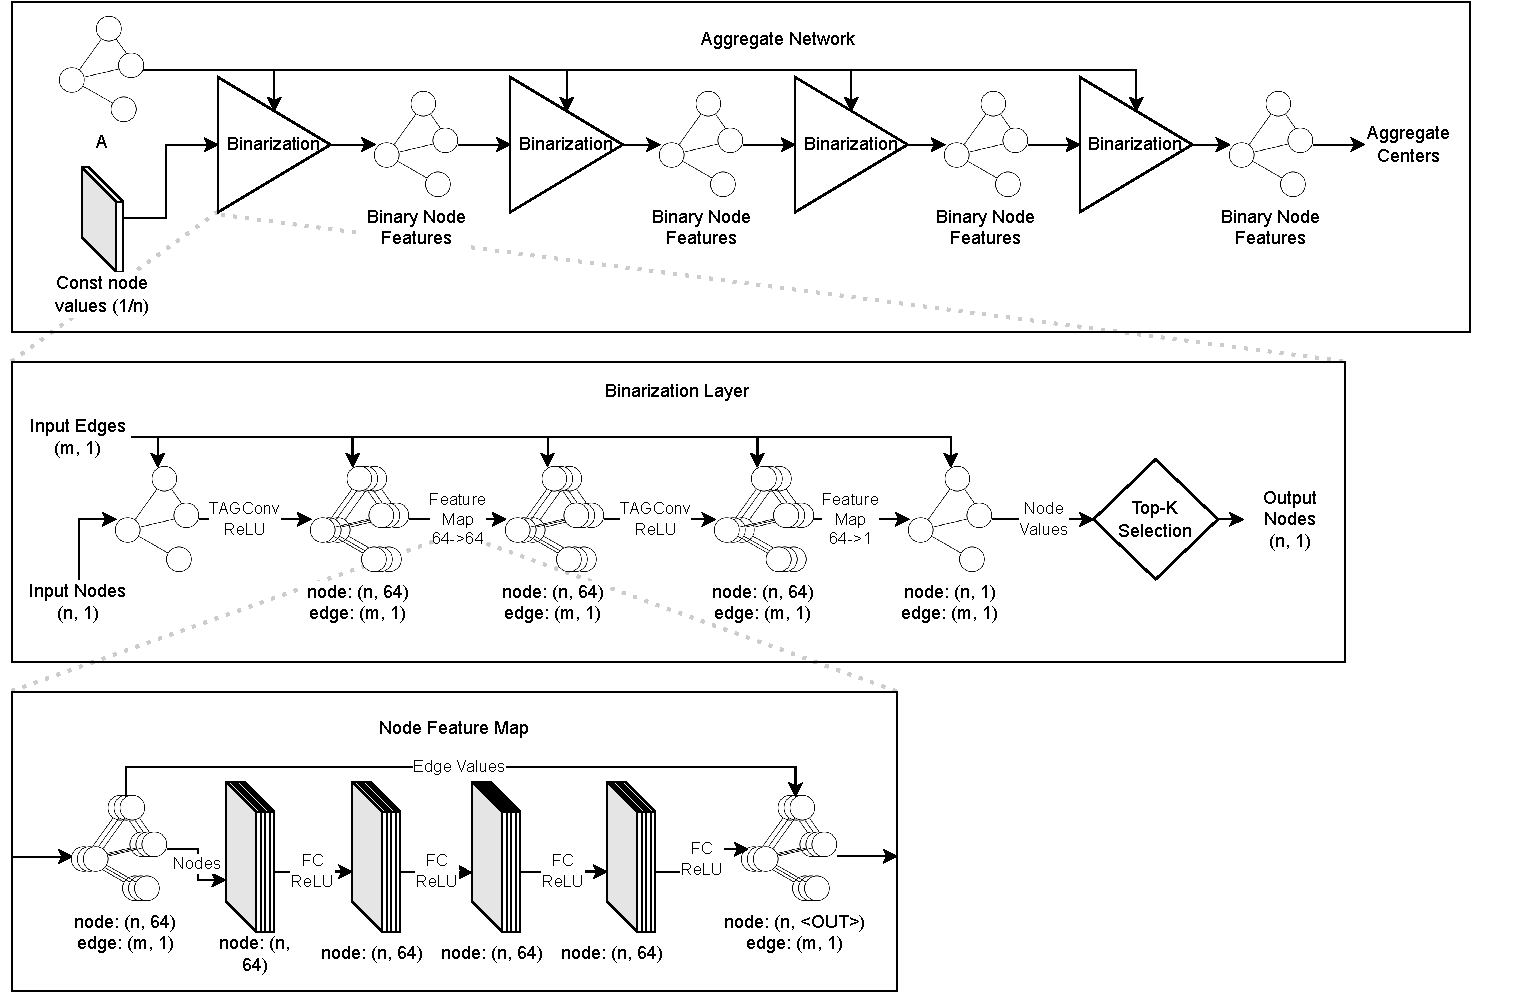
\includegraphics[width=\textwidth]{aggregate.pdf}
  \caption{Architecture for the aggregate-picking network.  This consists of 4 binarization layers, each having two node convolution passes.}
  \label{fig:arch_agg}
\end{figure}

To compute the aggregates and final interpolation operator, we concurrently train three graph networks to give different outputs:
\begin{enumerate}
\item $\Theta_{\text{agg}}$, outputting aggregate centers
\item $\Theta_{\text{soc}}$, outputting a strength-of-connection matrix for Bellman-Ford
\item $\Theta_{P}$, outputting a smoothing operator
\end{enumerate}
The algorithm for computing the interpolation operator is roughly sketched below:
\begin{enumerate}
\item Let $\mat{A} \in \mathbb{R}^{n \times n}$ be the system we are trying to solve and $\alpha \in \left(0, 1\right]$ be some parameter that determines the ratio of aggregates to vertices, i.e. we will be roughly coarsening the graph by $1/\alpha$.  Define $k := \ceil{\alpha n}$, the number of aggregates we will be outputting.
\item Convolve the graph of $\mat{A}$ with $\Theta_{\text{soc}}$ to obtain $\mat{C}$, a matrix of weights that will be used for Bellman-Ford.
\item Convolve the graph of $\mat{A}$ concatenated with $\mat{C}$ using $\Theta_{\text{agg}}$ to obtain a new set of node values, restarting multiple times and inserting the tenative cluster centers as a node feature.  We will use the output node values as a \textit{scoring}.  Define the aggregate centers as the indices of the largest $k$ node scores.
\item Run Bellman-Ford on the graph with these aggregate centers to obtain a tentative aggregation operator, $\text{Agg}$.
\item Now, again convolve the graph of $\mat{A}$ but with $\Theta_{\text{Interp}}$ (with aggregate information) to obtain the aggregate smoother $\mat{\hat{P}}$.  Form $\mat{P} := \mat{\hat{P}}\text{Agg}$.
\end{enumerate}
These steps are formalized in Alg \ref{alg:algo}.

\begin{algorithm}
  \begin{algorithmic}
    \Procedure{FullAggNet}{$\mat{A}\in\mathbb{R}^{n \times n}, \alpha$}
    \State $k := \ceil{\alpha n}$ \Comment{Number of aggregates to choose}
    \State $\mat{C} := \Theta_{\text{soc}}\left(\mat{A}\right)$ \Comment{Obtain strength-of-connection matrix}
    \\
    \State $\vec{s} := \Theta_{\text{agg}}\left(\mat{A}, \mat{C}, k\right)$ \Comment{Get aggregate scores for each node}
    \State $\vec{r} := $ \Call{top-k}{$\vec{s}, k$} \Comment{Get indices of $k$ largest nodes to be centers}
    \State $\mat{\text{Agg}} := $ \Call{Bellman-Ford}{$\mat{C}, \vec{r}$} \Comment{Get tentative aggregate assignment matrix}
    \\
    \State $\mat{\hat{P}} := \Theta_{\text{Interp}}\left(\mat{A}, \mat{\text{Agg}}\right)$ \Comment{Aggregate smoother}
    \State \Return $\mat{\hat{P}} \mat{\text{Agg}}$ \Comment{Smooth aggregate assignment}
    \EndProcedure
  \end{algorithmic}
  \caption{Outputting Aggregates and Interpolation}
  \label{alg:algo}
\end{algorithm}

\section{Genetic Training}
Training of both networks is done at the same time with a custom-written genetic algorithm that takes advantage of the easily parallelizable fitness calculation.  A genetic algorithm is used because it does not require any gradient information, which benefits us because the algorithm used to output the aggregates is not easily differentiable.

A basic overview of the training algorithm is that the method is seeded with some number of randomly generated networks. A subset of the best performing (most fit) networks are selected and \textit{bred} with one another (crossing weights/traits) and \textit{mutations} inserted (random perturbations to weights) to create another population of networks.  This is then repeated for many \textit{generations} until a set of hopefully trained networks is obtained, from which we can pick the best fit as our final network.

\subsection{Folded Crossover}
So-called ``folded crossover'', as explored in \cite{GA_CNN}, is a genetic crossover technique that groups together consistent regions of the population's chromosomes.  When training neural networks, it is entirely possible that specific modules (layers) can contain several hundred or even several thousand weight entries, meaning traditional crossover that na\"ively slice arbitrary points of the weight space can partially replace weight values for modules and produce suboptimal offspring.

By ``folding'' regions of the weight space, we ensure that whole modules are copied to offspring.  We further modify the crossover procedure by allowing the two children of a pair of parents to randomly pick which parent they receive each module from.  This is an additional level of flexibility compared to, e.g., single-point or two-point crossover which divide the weight-space into two or three regions, respectively.

Initial testing of the folded crossover provides subjective speedup to the rate at which networks learn, but I haven't really timed it or anything.

\subsection{Stochastic Batching}
As mentioned previously, the most expensive part of training the networks is the computation of the fitness values, as we must compute an average convergence rate over every mesh in our training set, for every network in our population.  Reducing the number of meshes used at each generation can drastically speed-up the training routine, at perhaps a reduction in training effectivity.  This also eliminates any notion of caching fitness values for regions of the population that do not change between generations, as we have a different batch each generation and must totally re-compute fitness to have any sort of reasonable comparison.

In practice, this gives a healthy speed-up for minibatch sizes of only $16$.  I had to decrease the maximum perturbation during mutation to $\abs{m}=0.1$ to get it to do anything sensible, but perhaps it was too high in the first place?

\subsection{Greedy Selection}
I've experimentally found that using steady-state selection will train the network up to some point, then completely fail to make any more progress.  At this point in the training, I've switched to what I call a \text{greedy selection}, where the population at generation $i+1$ will totally consist of the one fittest individual from $i$.  Then, these will be mutated as usual.

I kind of think of this as a sort of greedy approximation to gradient descent: we have one network and at every step we attempt to take the most optimal step towards a better network.

\section{Baseline Lloyd Method}
The baseline method for computing some multigrid smoothing operator is given by \textit{Lloyd aggregation}, the implementation of which was taken from PyAMG\cite{OlSc2018}.  This algorithm returns a tentative aggregate operator, $\mat{\text{Agg}}$.  Afterwards, a Jacobi smoother is formed by
\begin{align}
  \mat{S} &:= \mat{I} - \omega\mat{D}^{-1}\mat{A}, \\
  \omega &:= \frac{4}{3\lambda_{\max}\left(\mat{A}\right)},
\end{align}
where $\mat{A}$ is the linear system to solve and $\mat{D}$ is the diagonal portion of $\mat{A}$.  The final interpolation is formed by
\begin{equation}
  \mat{P} = \mat{S} \mat{\text{Agg}}.
\end{equation}

\section{Results}
The ML method is compared against a baseline Lloyd aggregation with Jacobi smoothing, for a coarsening ratio of $\alpha=0.1$.  Performance is measured by \textit{average rate of convergence} for some set of problems; detailed information is given in table \ref{tab:conv}.

\begin{table}[h]
  \centering
  \begin{tabular}{c c c c}
    \textbf{Problem Type} & \textbf{Data Set} & \textbf{Lloyd, SA Conv.} & \textbf{ML Conv.} \\
    \hline
    Isotropic & Train & 0.4208 & 0.4109 \\
    Isotropic & Test & 0.4177 & 0.4075 \\
    Anisotropic & Train & 0.7705 & 0.7451 \\
    Anisotropic & Test & 0.7978 & 0.7697 \\
    \hline
  \end{tabular}
  \caption{Convergence of ML vs baseline Lloyd+SA on various sets of problems.}
  \label{tab:conv}
\end{table}

\FloatBarrier
\subsection{Isotropic Results}

\begin{figure}[h]
  \centering
  \begin{subfigure}[t]{0.49\textwidth}
    \centering
    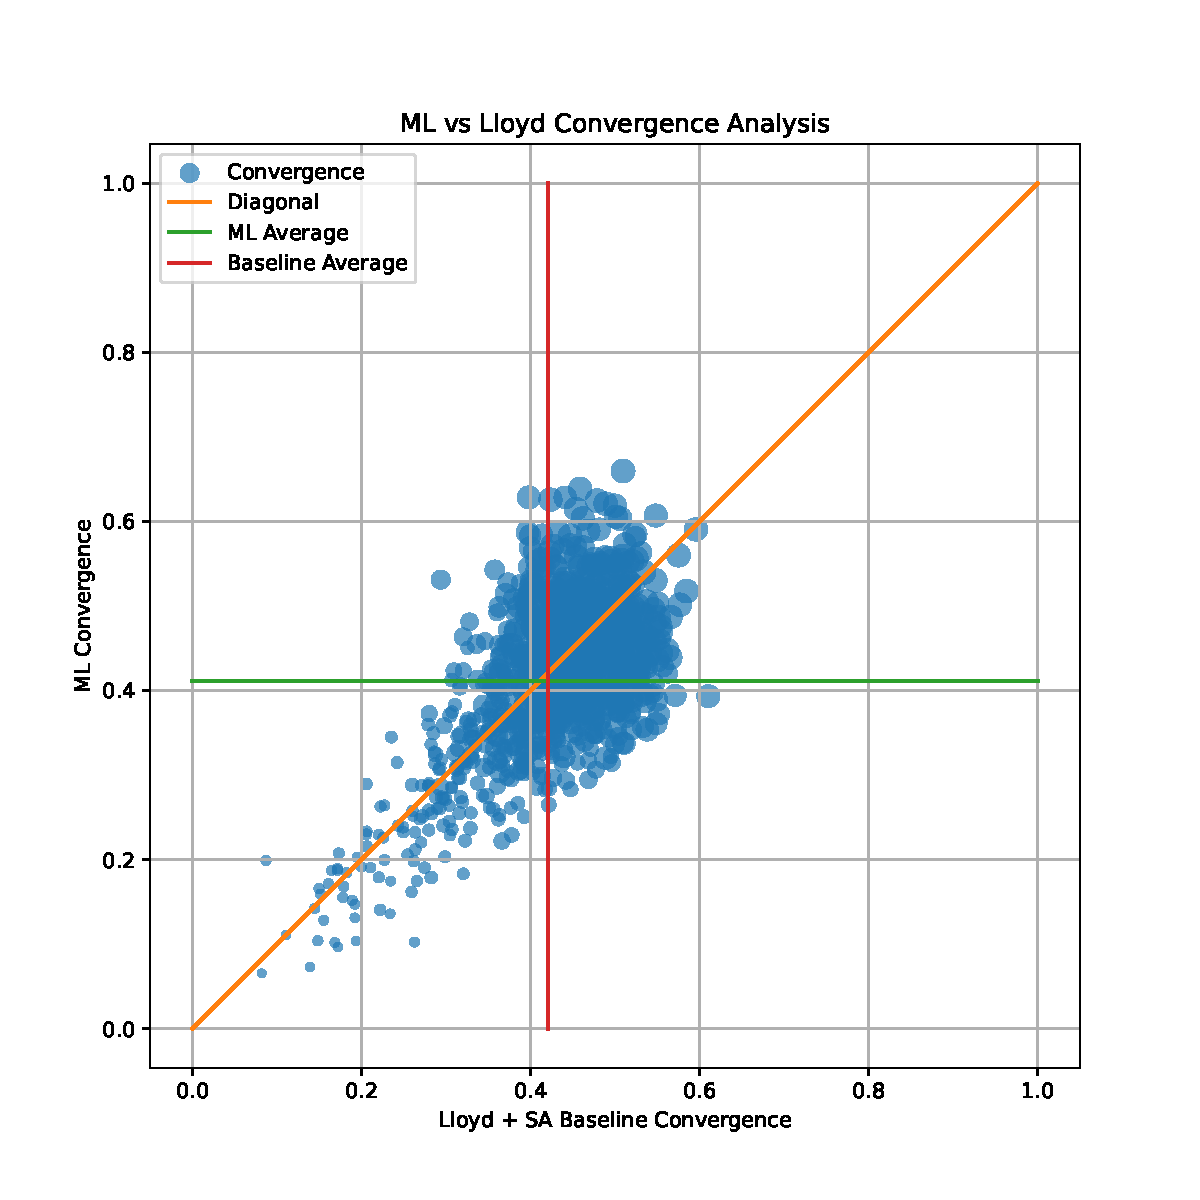
\includegraphics[width=\textwidth]{iso_train_convergence.pdf}
    \caption{Training convergence}
  \end{subfigure}
  \begin{subfigure}[t]{0.49\textwidth}
    \centering
    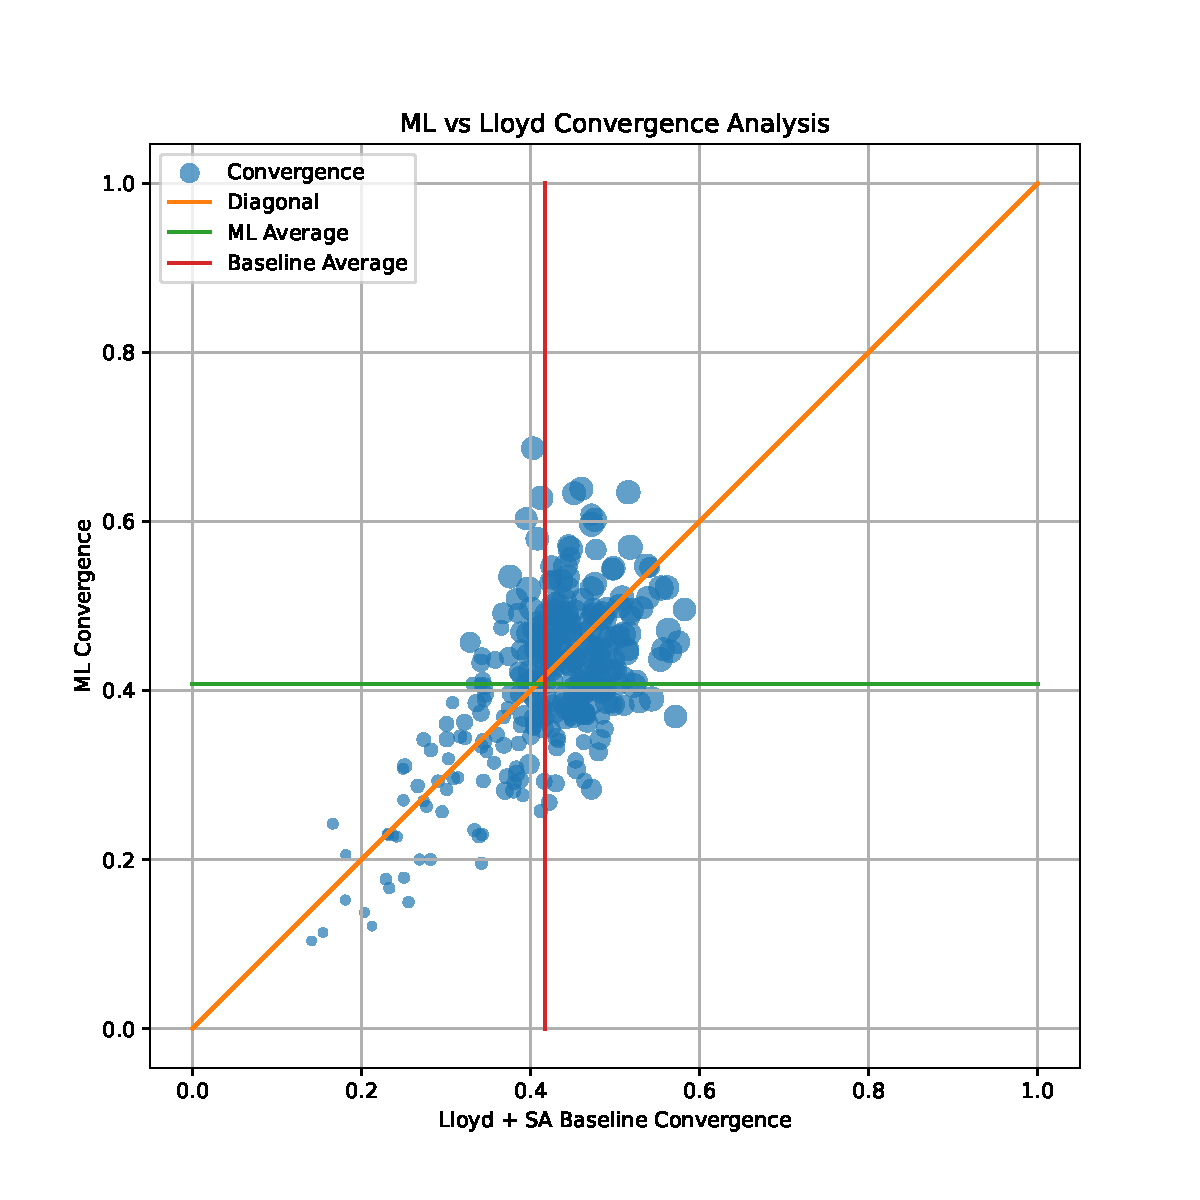
\includegraphics[width=\textwidth]{iso_test_convergence.pdf}
    \caption{Testing convergence}
  \end{subfigure}
  \caption{Convergence data for the ML AMG method vs a baseline Lloyd and Jacobi SA method.  Values below the diagonal indicate a better convergence for the ML.  Markers are scaled by problem size.}
  \label{fig:conv}
\end{figure}

\begin{figure}[h]
  \centering
  \begin{subfigure}[t]{0.49\textwidth}
    \centering
    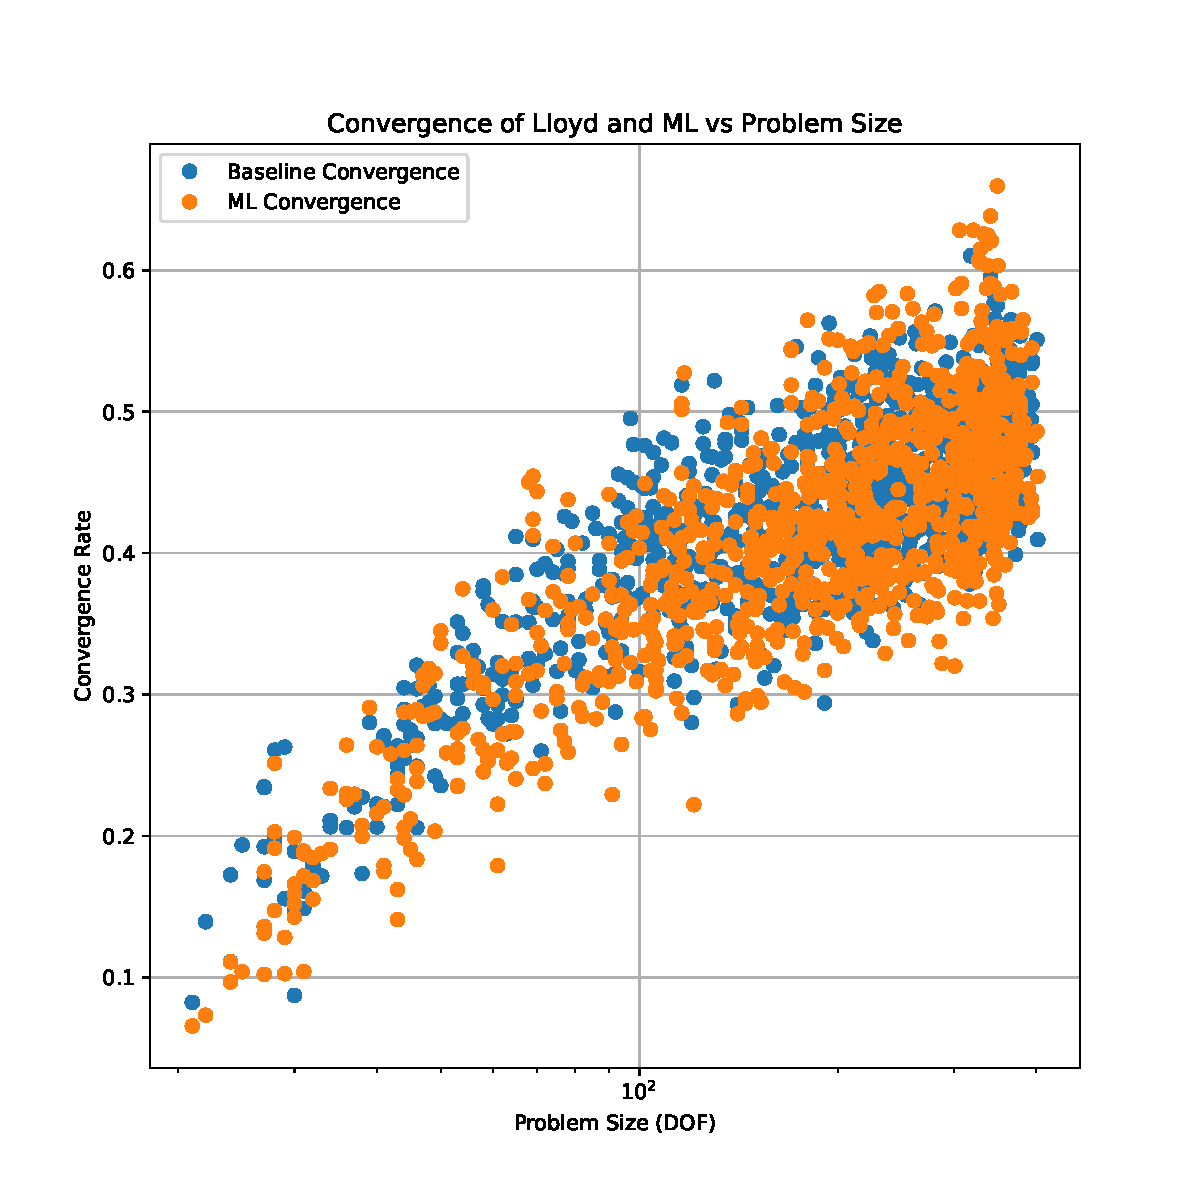
\includegraphics[width=\textwidth]{iso_train_convergence_per_size.pdf}
    \caption{Training convergence}
  \end{subfigure}
  \begin{subfigure}[t]{0.49\textwidth}
    \centering
    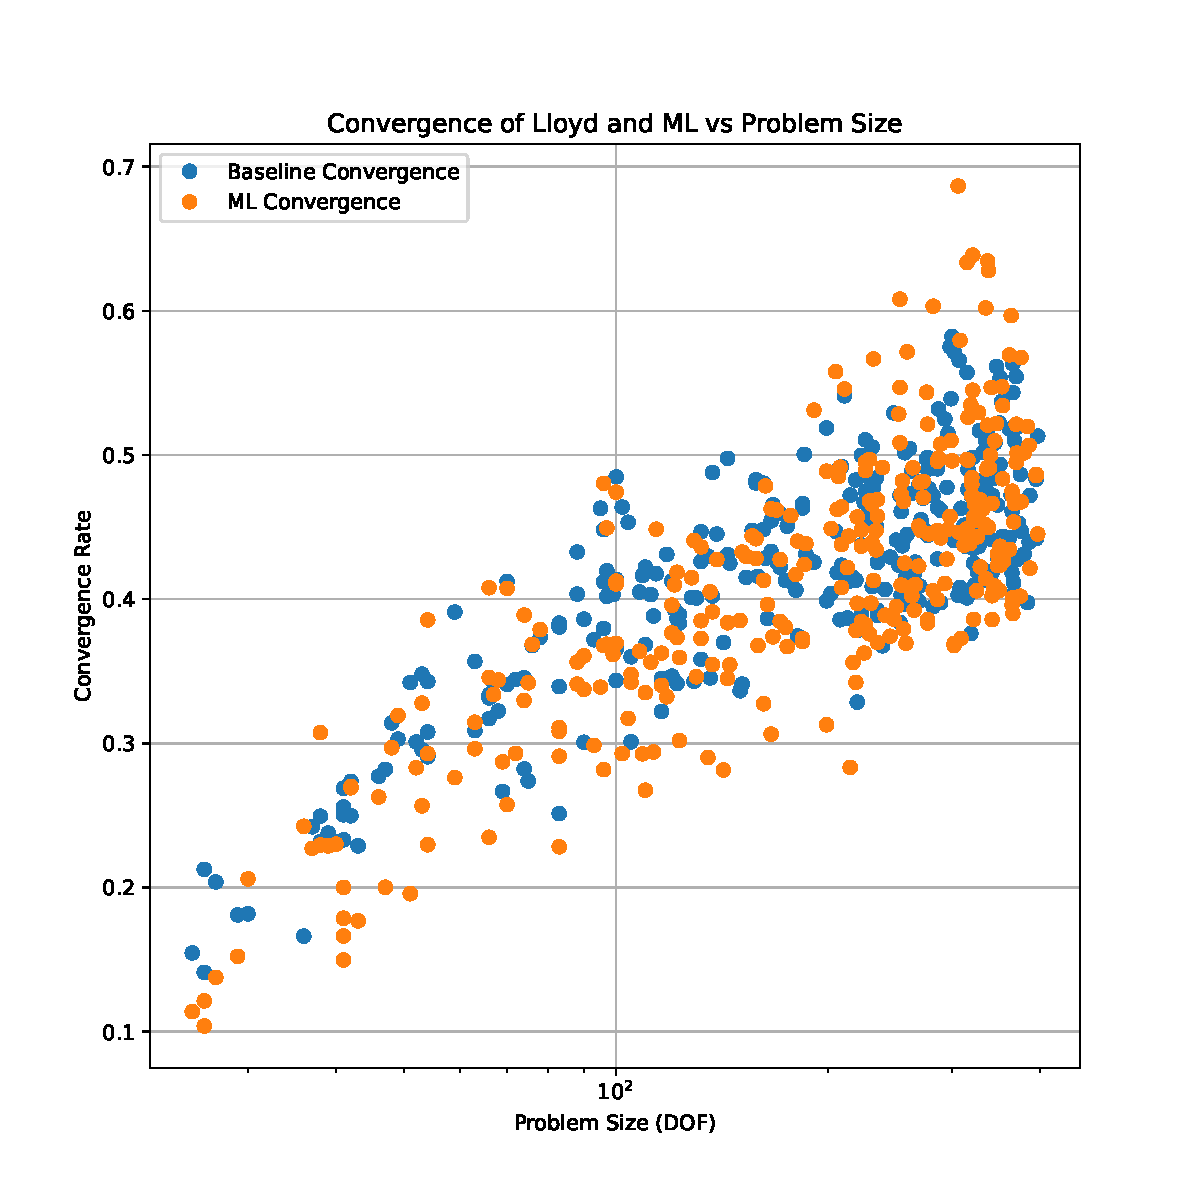
\includegraphics[width=\textwidth]{iso_test_convergence_per_size.pdf}
    \caption{Testing convergence}
  \end{subfigure}
  \caption{Convergence data for the two methods plotted against problem size (DOF).}
  \label{fig:conv_per_size}
\end{figure}

\begin{figure}[h]
  \centering
  \begin{subfigure}[t]{0.49\textwidth}
    \centering
    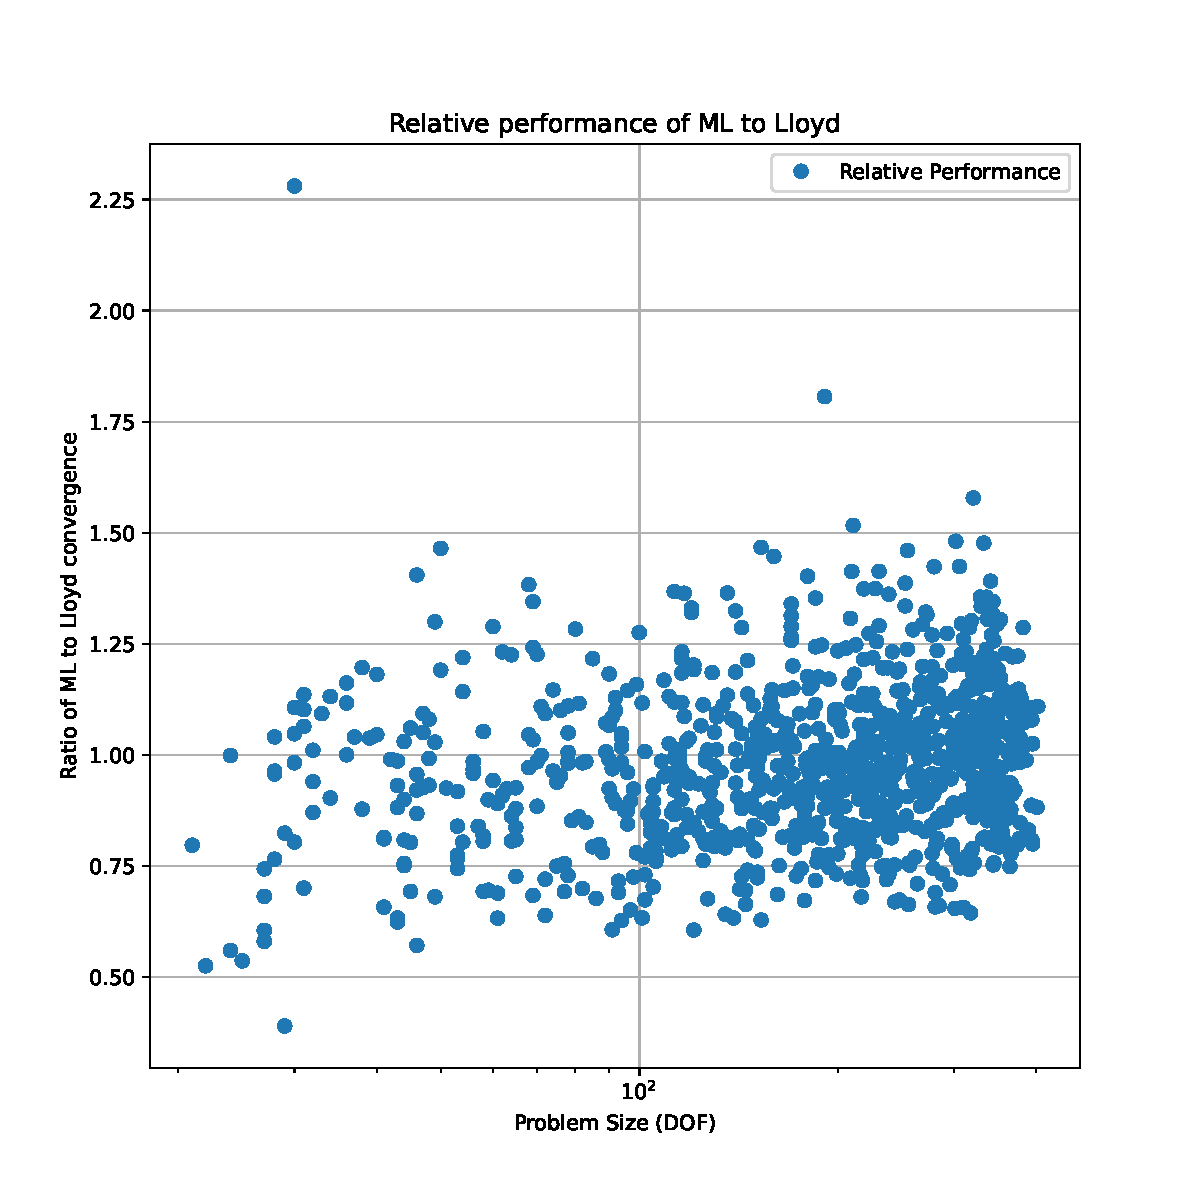
\includegraphics[width=\textwidth]{iso_rel_perf_train.pdf}
    \caption{Relative training performance}
  \end{subfigure}
  \begin{subfigure}[t]{0.49\textwidth}
    \centering
    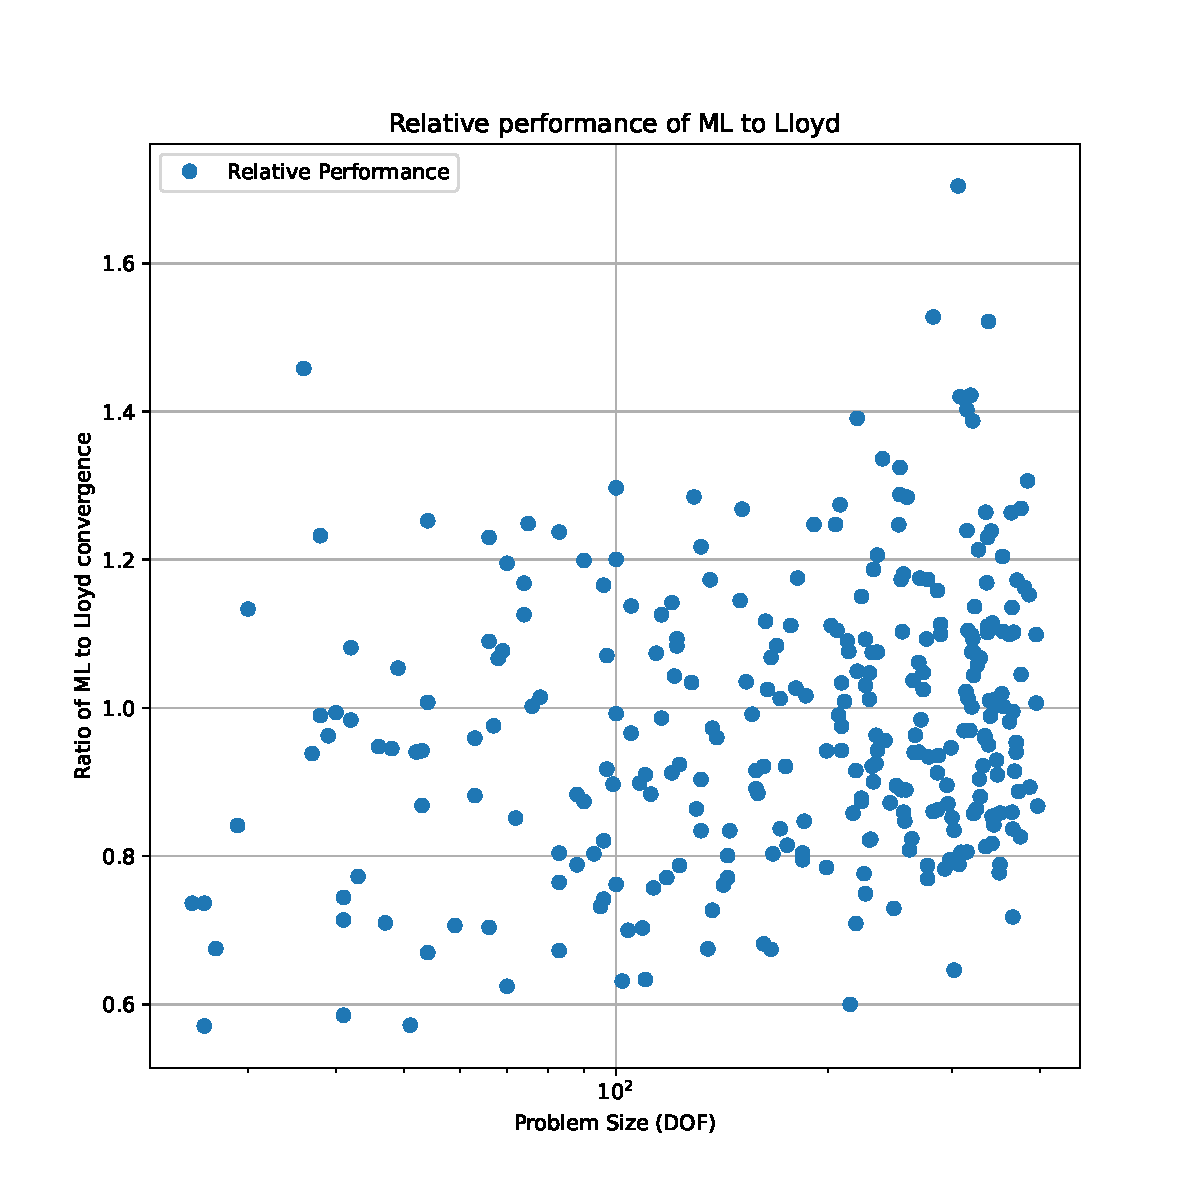
\includegraphics[width=\textwidth]{iso_rel_perf_test.pdf}
    \caption{Relative testing performance}
  \end{subfigure}
  \caption{Relative performance of the ML to the Lloyd method, plotted against problem size.  Relative performance is obtained by dividing the ML convergence by the Lloyd convergence for each problem.  Values below $1$ indicate better ML performance, while values above $1$ indicate better baseline performance.}
  \label{fig:rel_conv}
\end{figure}

\begin{figure}[h]
  \centering
  \begin{subfigure}[t]{0.32\textwidth}
    \centering
    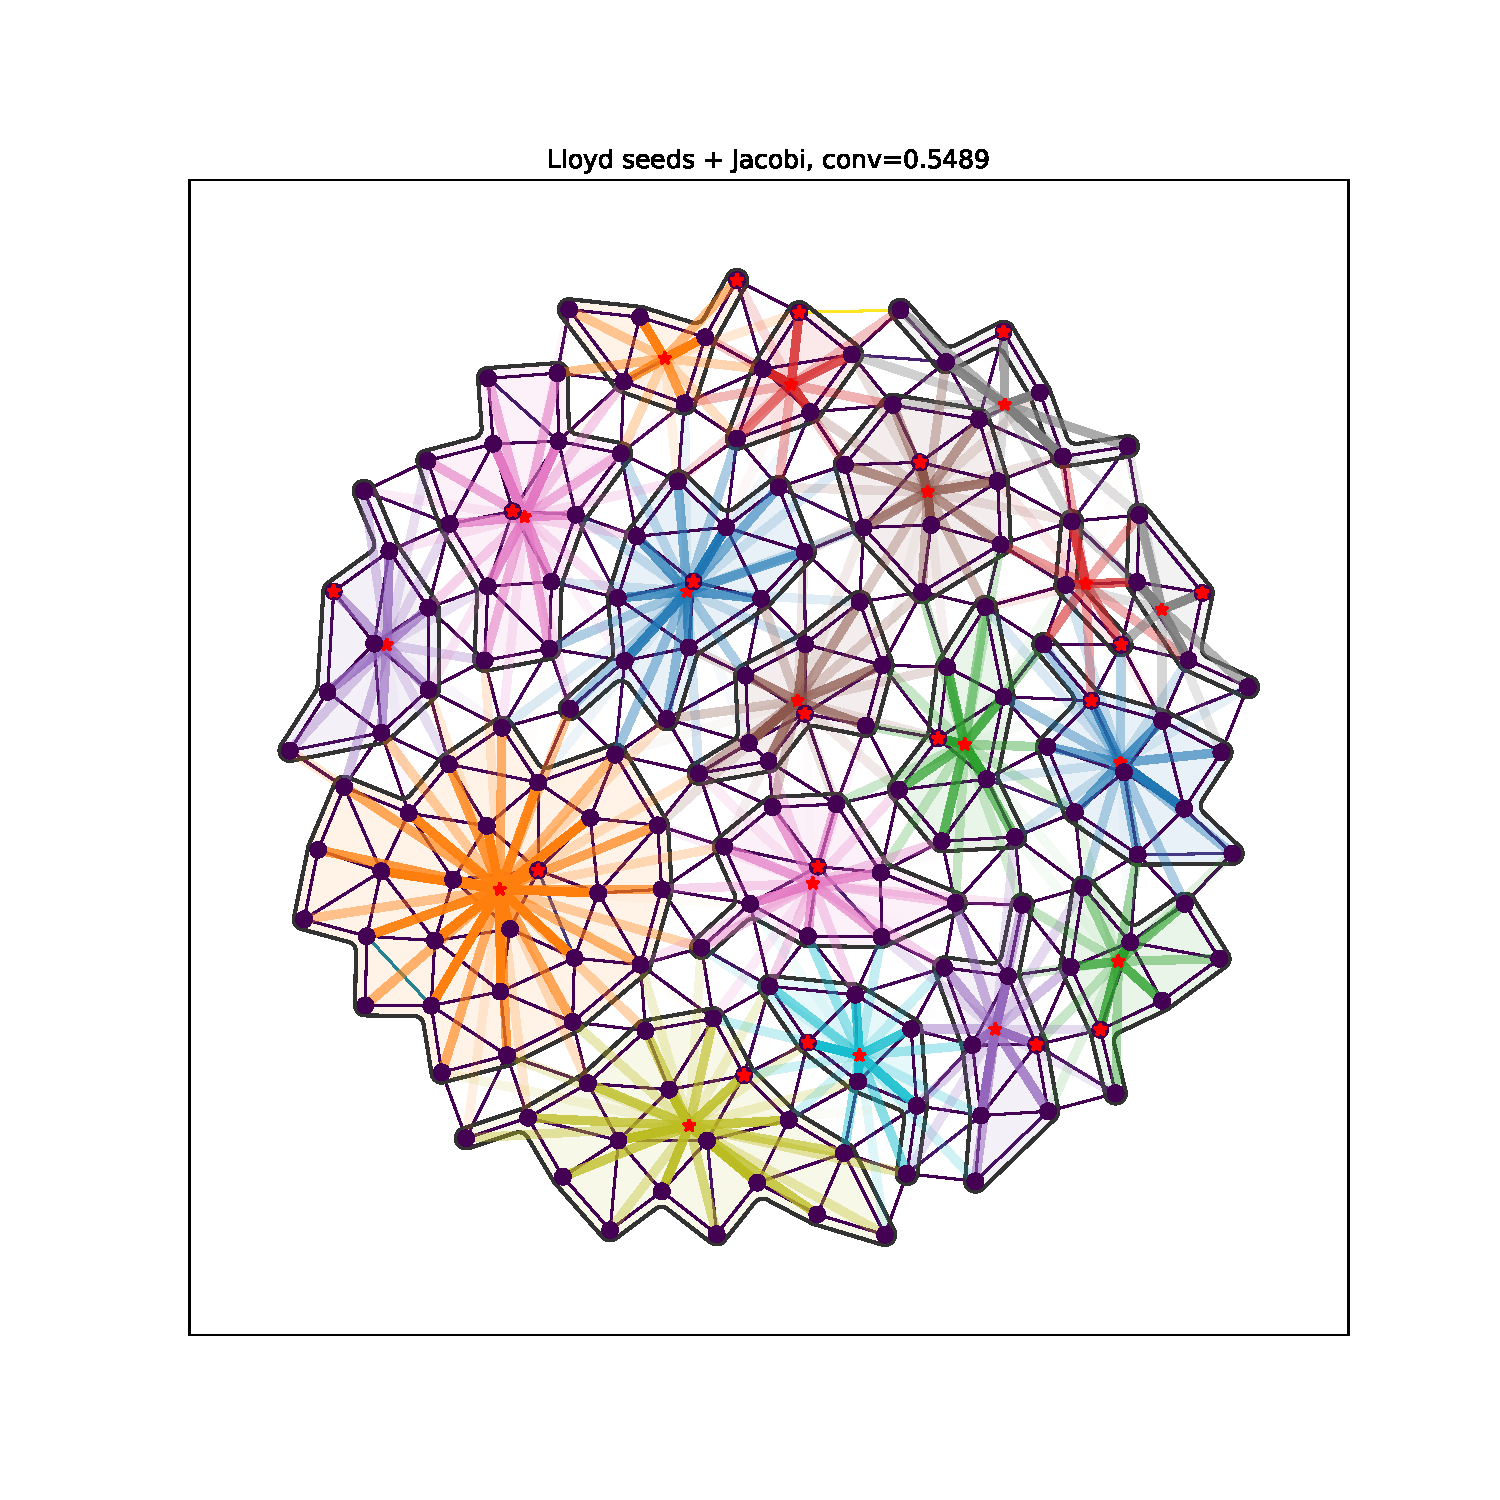
\includegraphics[width=\textwidth, trim=80 70 70 50, clip]{grid_circle_dumb.pdf}
    \caption{Initial Lloyd Configuration}
  \end{subfigure}
  \begin{subfigure}[t]{0.32\textwidth}
    \centering
    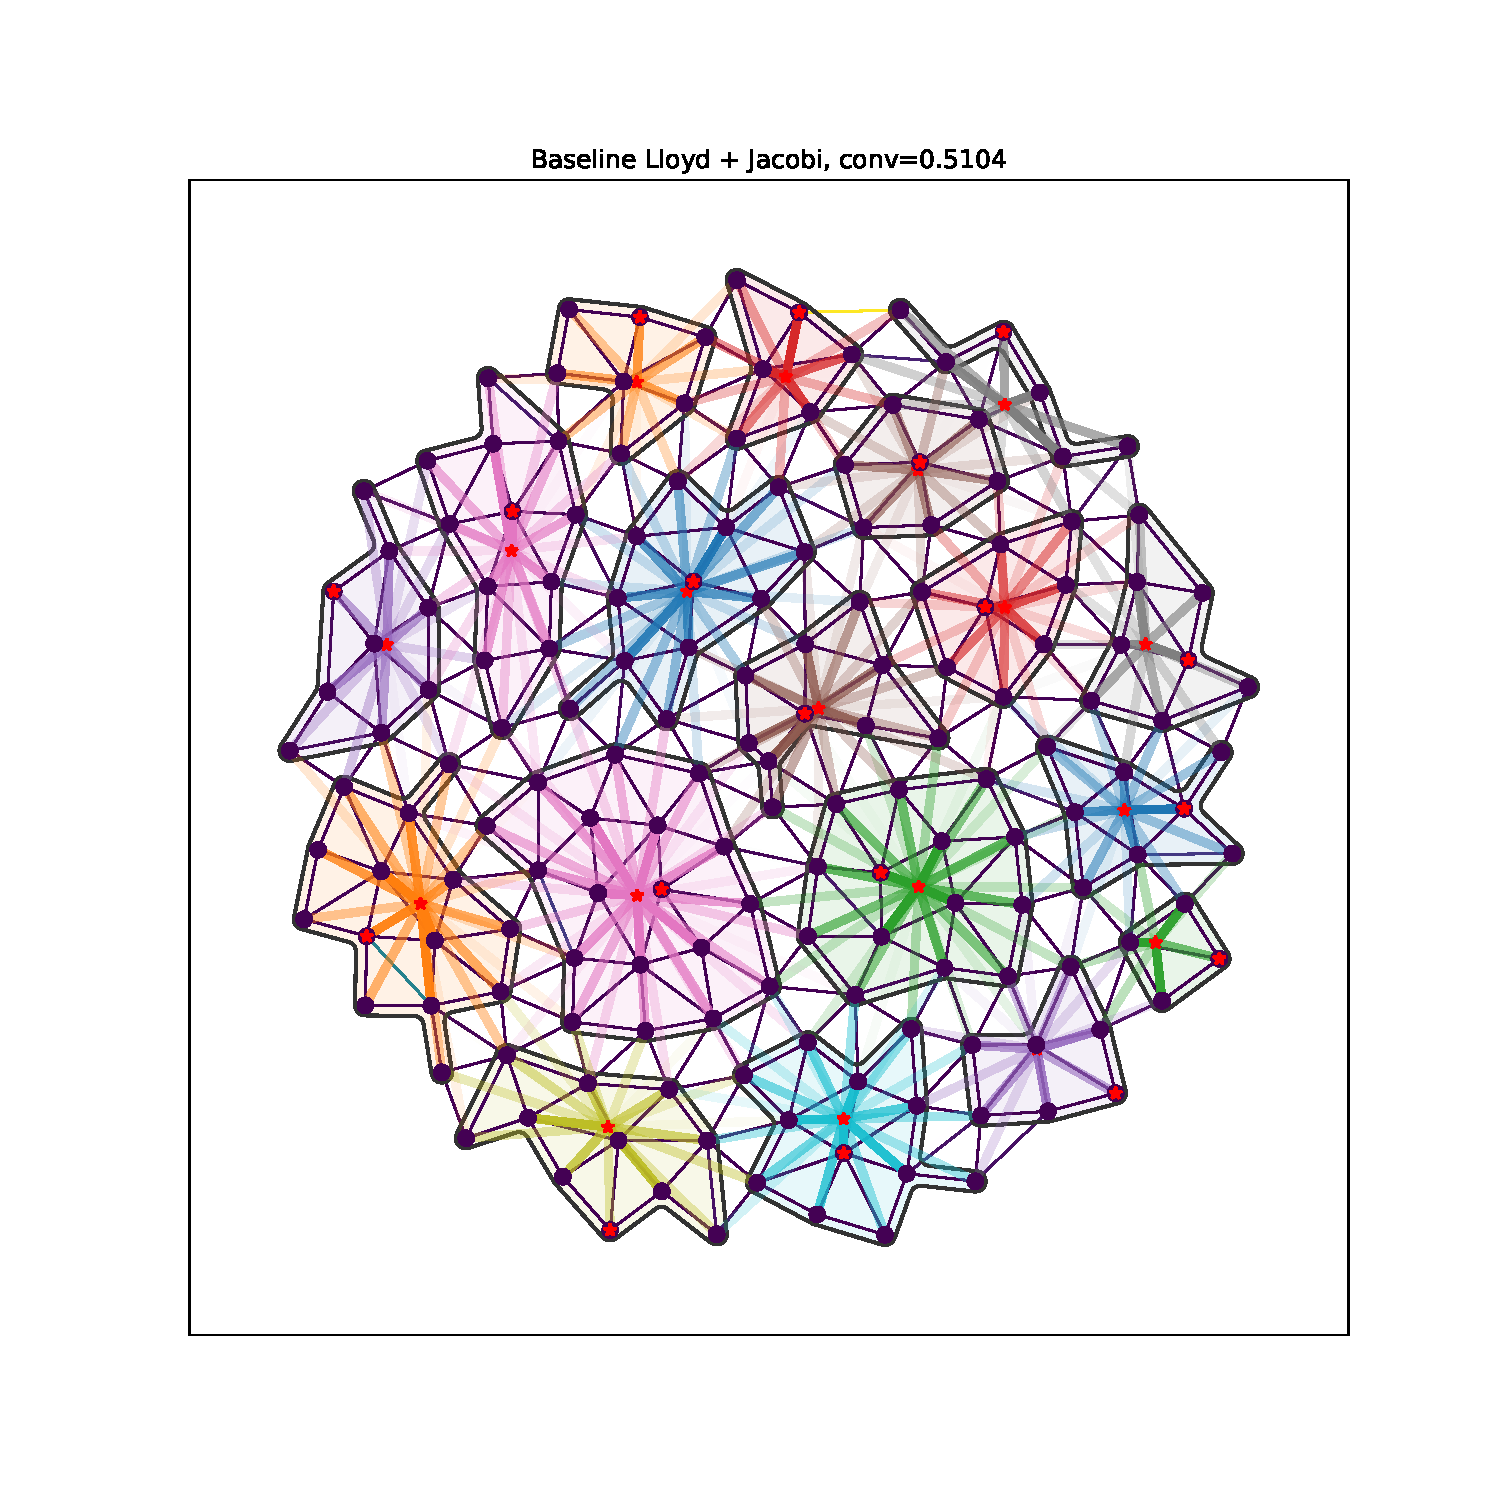
\includegraphics[width=\textwidth, trim=80 70 70 50, clip]{grid_circle_lloyd.pdf}
    \caption{Lloyd + Jacobi}
  \end{subfigure}
  \begin{subfigure}[t]{0.32\textwidth}
    \centering
    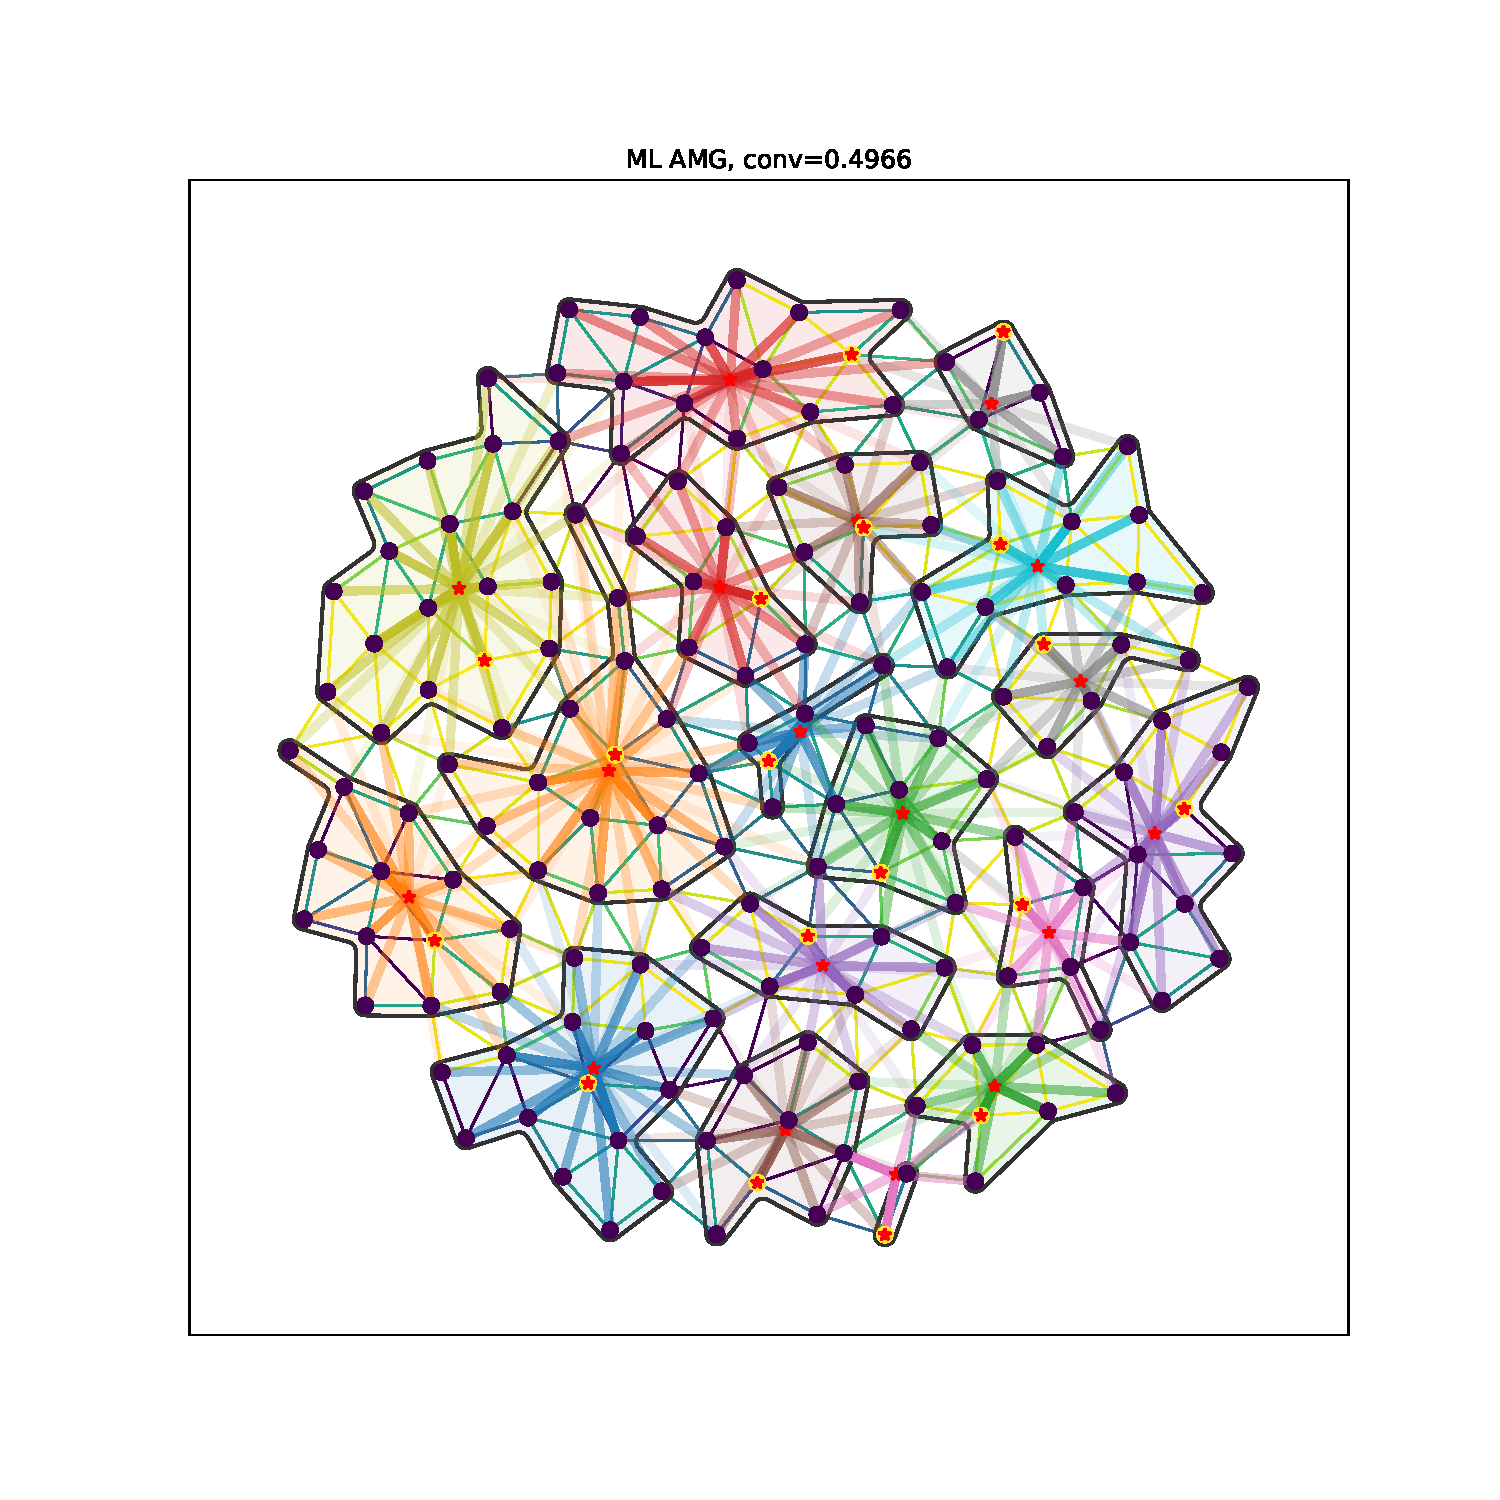
\includegraphics[width=\textwidth, trim=80 70 70 50, clip]{grid_circle_ml.pdf}
    \caption{ML}
  \end{subfigure}
  \caption{Aggregate and interpolation data for a circular unstructured mesh.  This particular mesh has 173 DoF.}
  \label{fig:gridcircle}
\end{figure}

\begin{figure}[h]
  \centering
  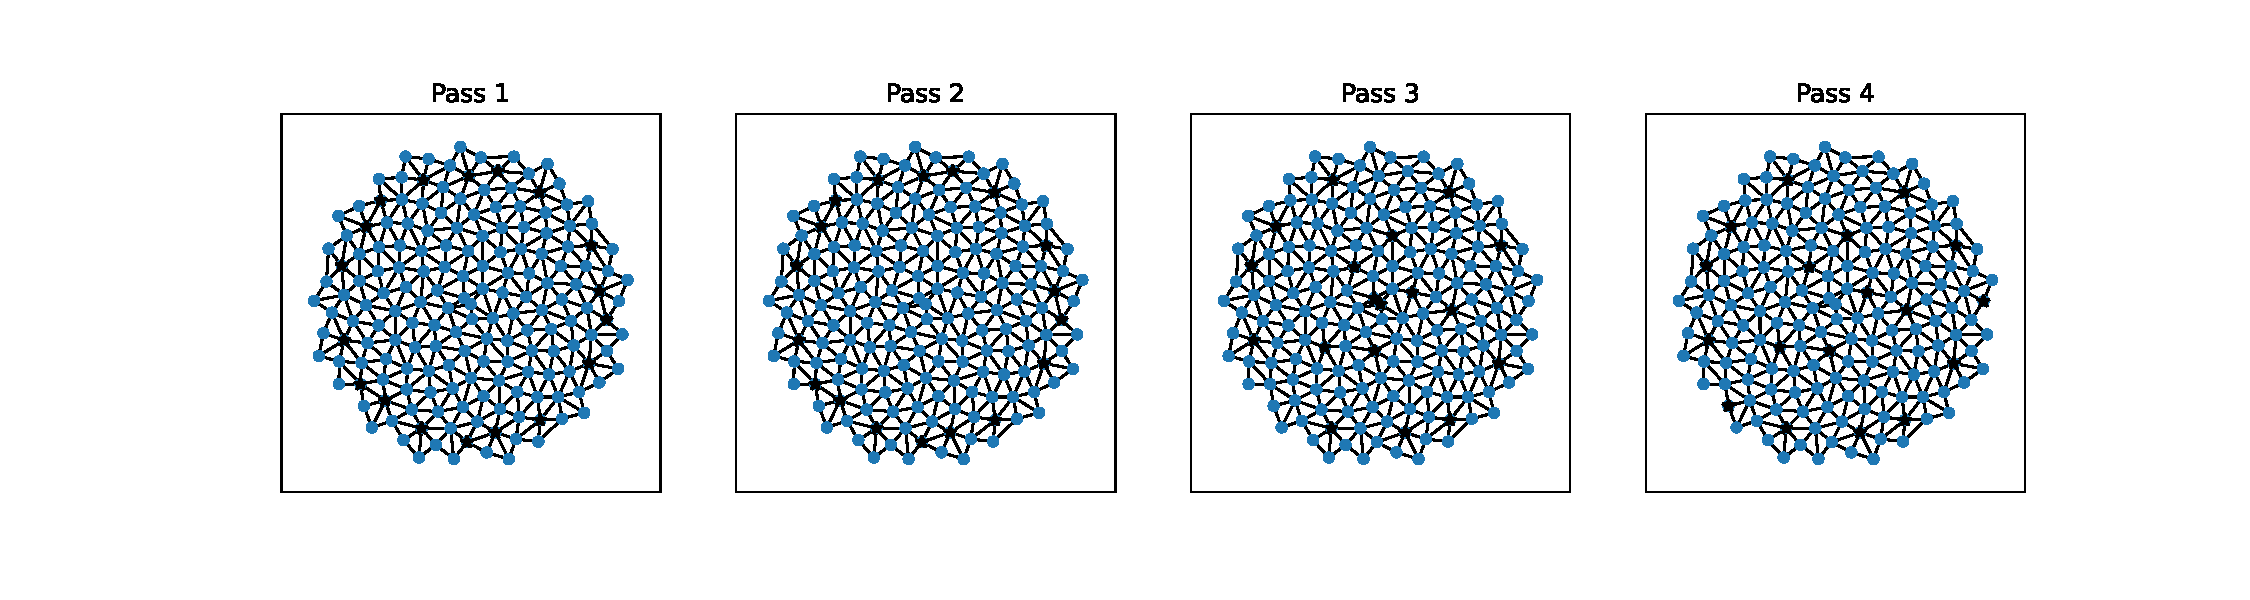
\includegraphics[width=\textwidth, trim=120 0 100 0, clip]{grid_circle_agg_pass.pdf}
  \caption{Tentative aggregate centers after each binarization ``pass''.  This is the same mesh as in figure \ref{fig:gridcircle}.}
\end{figure}

\begin{figure}[h]
  \centering
  \begin{subfigure}[t]{0.32\textwidth}
    \centering
    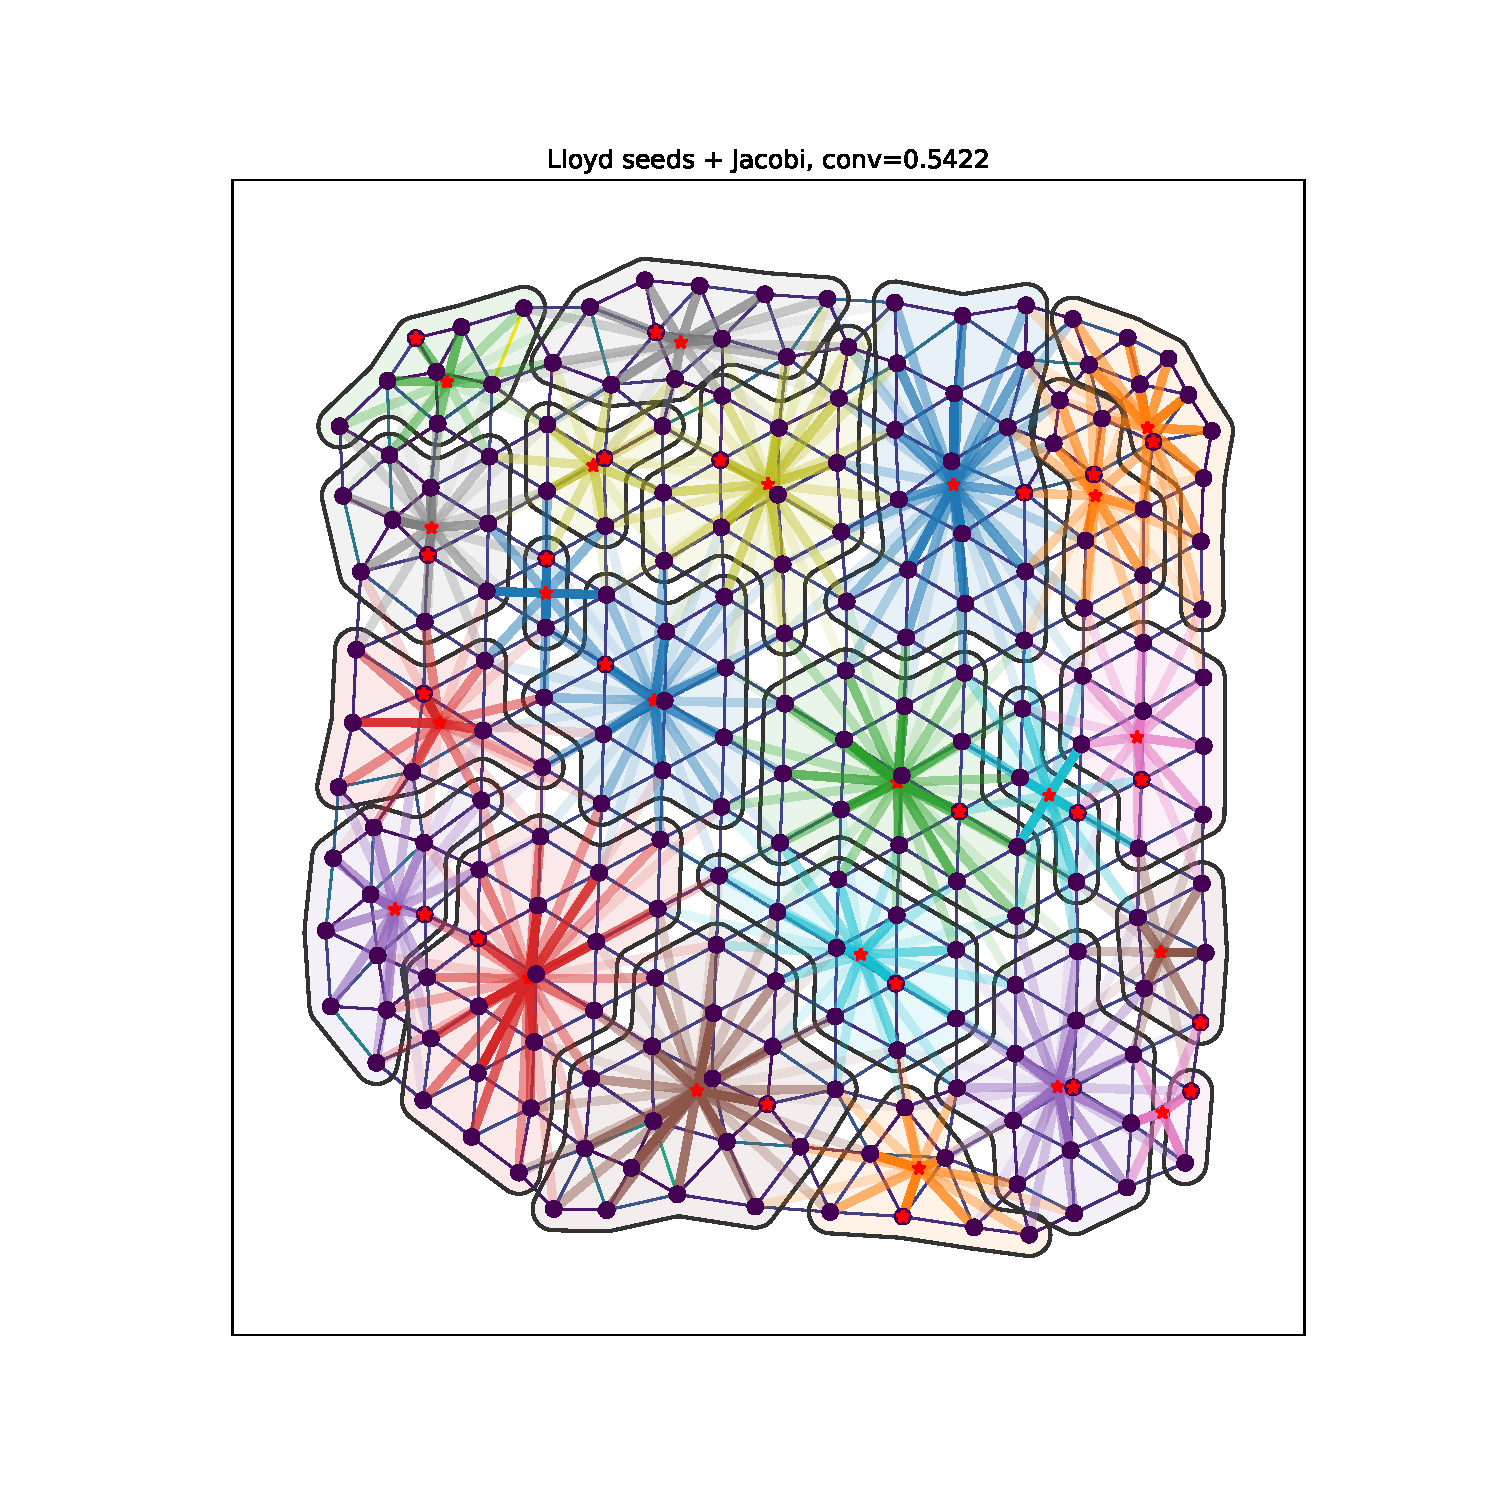
\includegraphics[width=\textwidth, trim=80 70 70 50, clip]{grid_700_dumb.pdf}
    \caption{Initial Lloyd Configuration}
  \end{subfigure}
  \begin{subfigure}[t]{0.32\textwidth}
    \centering
    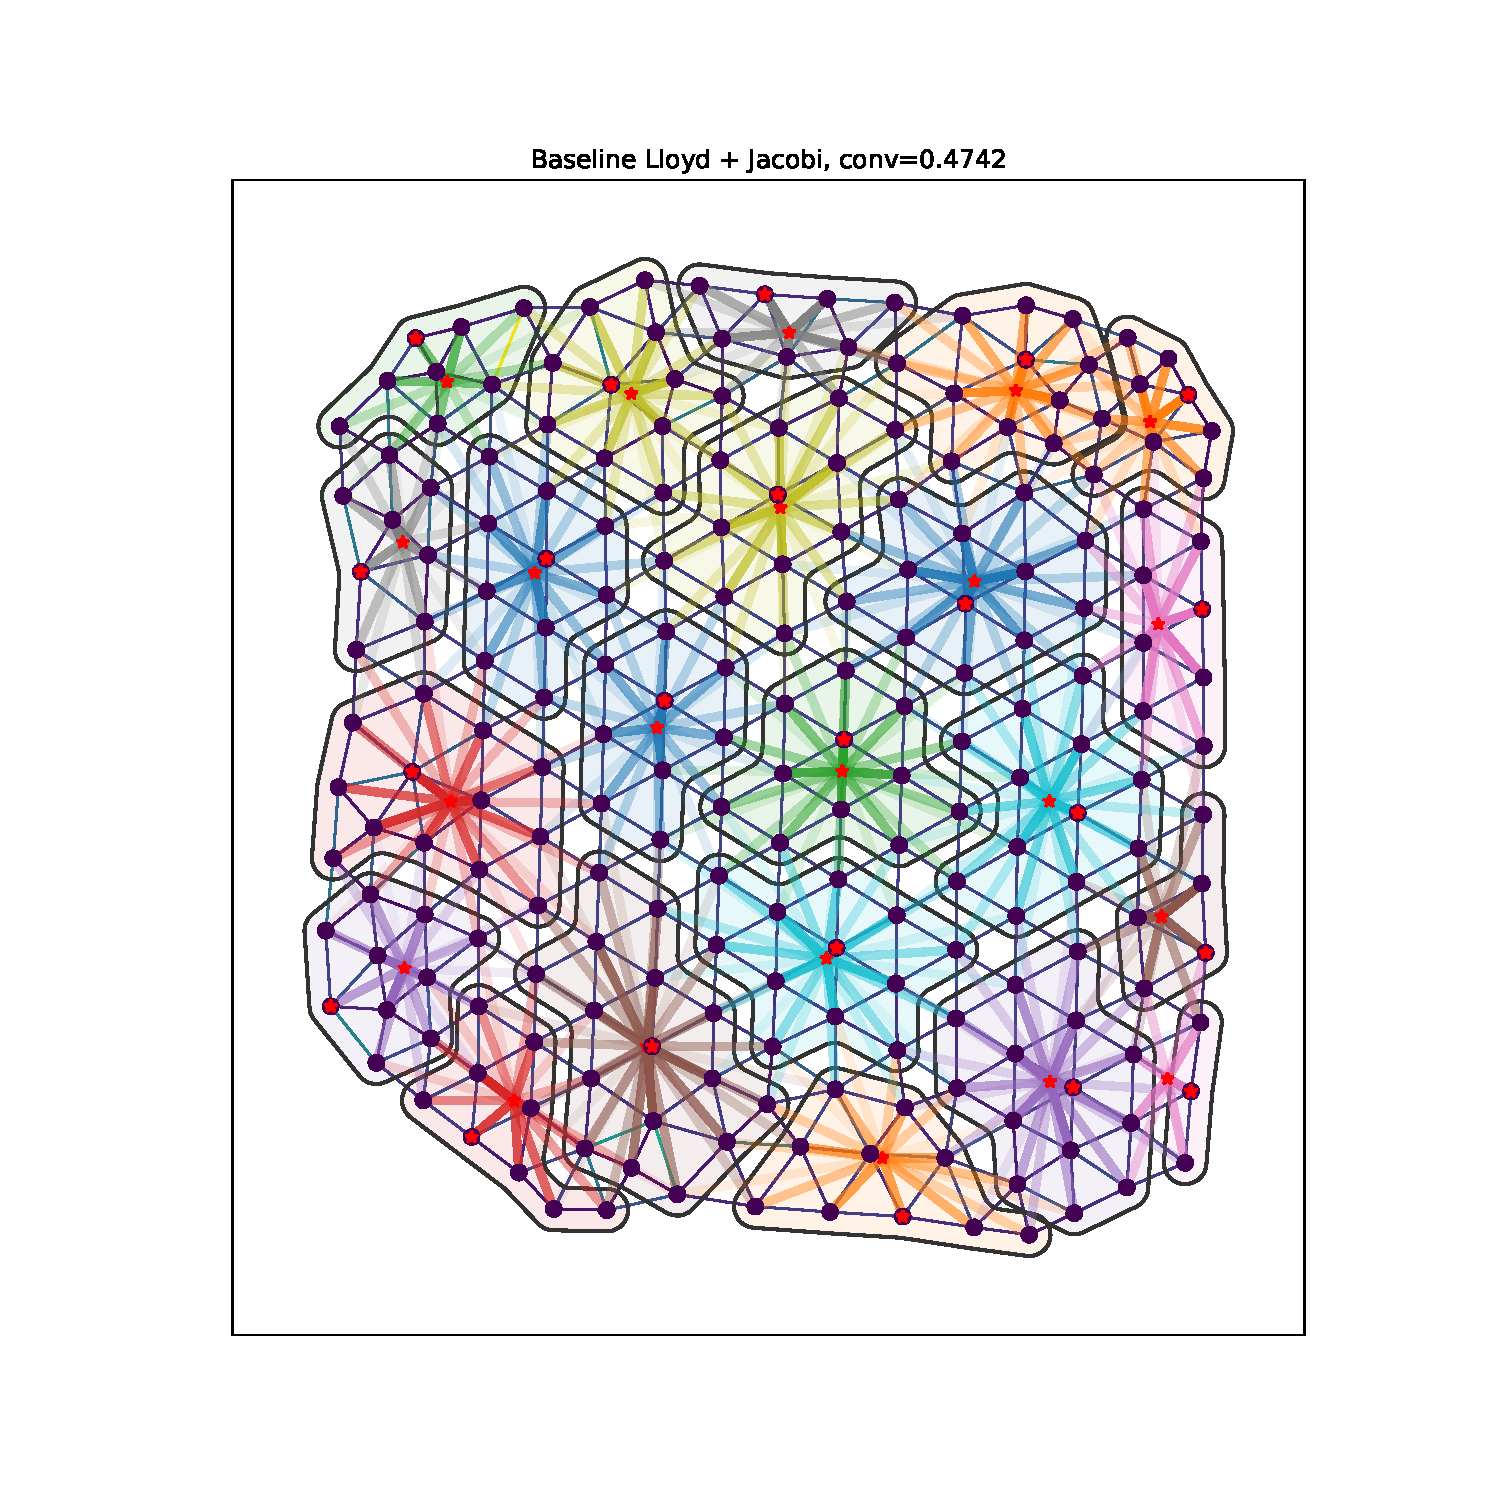
\includegraphics[width=\textwidth, trim=80 70 70 50, clip]{grid_700_lloyd.pdf}
    \caption{Lloyd + Jacobi}
  \end{subfigure}
  \begin{subfigure}[t]{0.32\textwidth}
    \centering
    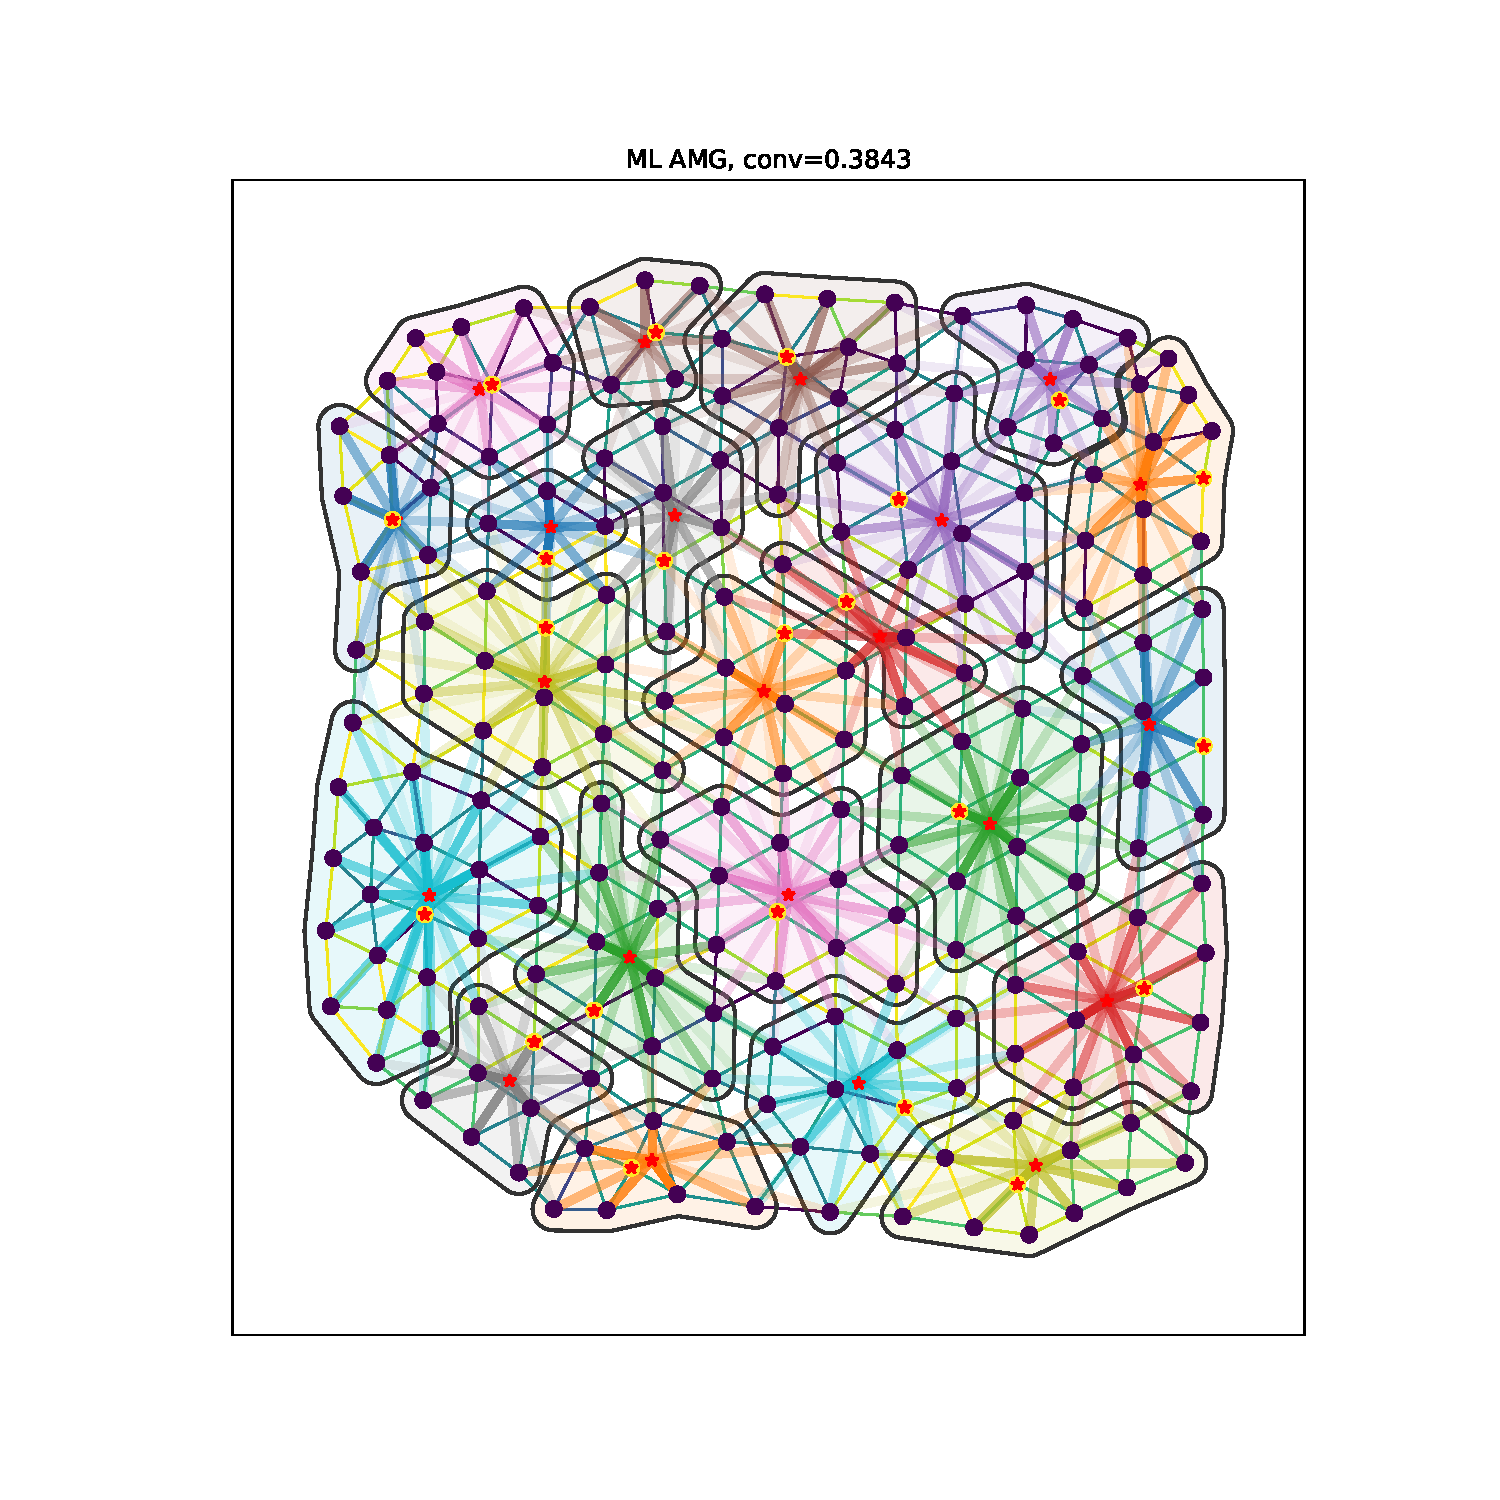
\includegraphics[width=\textwidth, trim=80 70 70 50, clip]{grid_700_ml.pdf}
    \caption{ML}
  \end{subfigure}
  \caption{Aggregate and interpolation data for a random unstructured mesh.  This particular mesh has 220 DoF.}
  \label{fig:grid700}
\end{figure}

\begin{figure}[h]
  \centering
  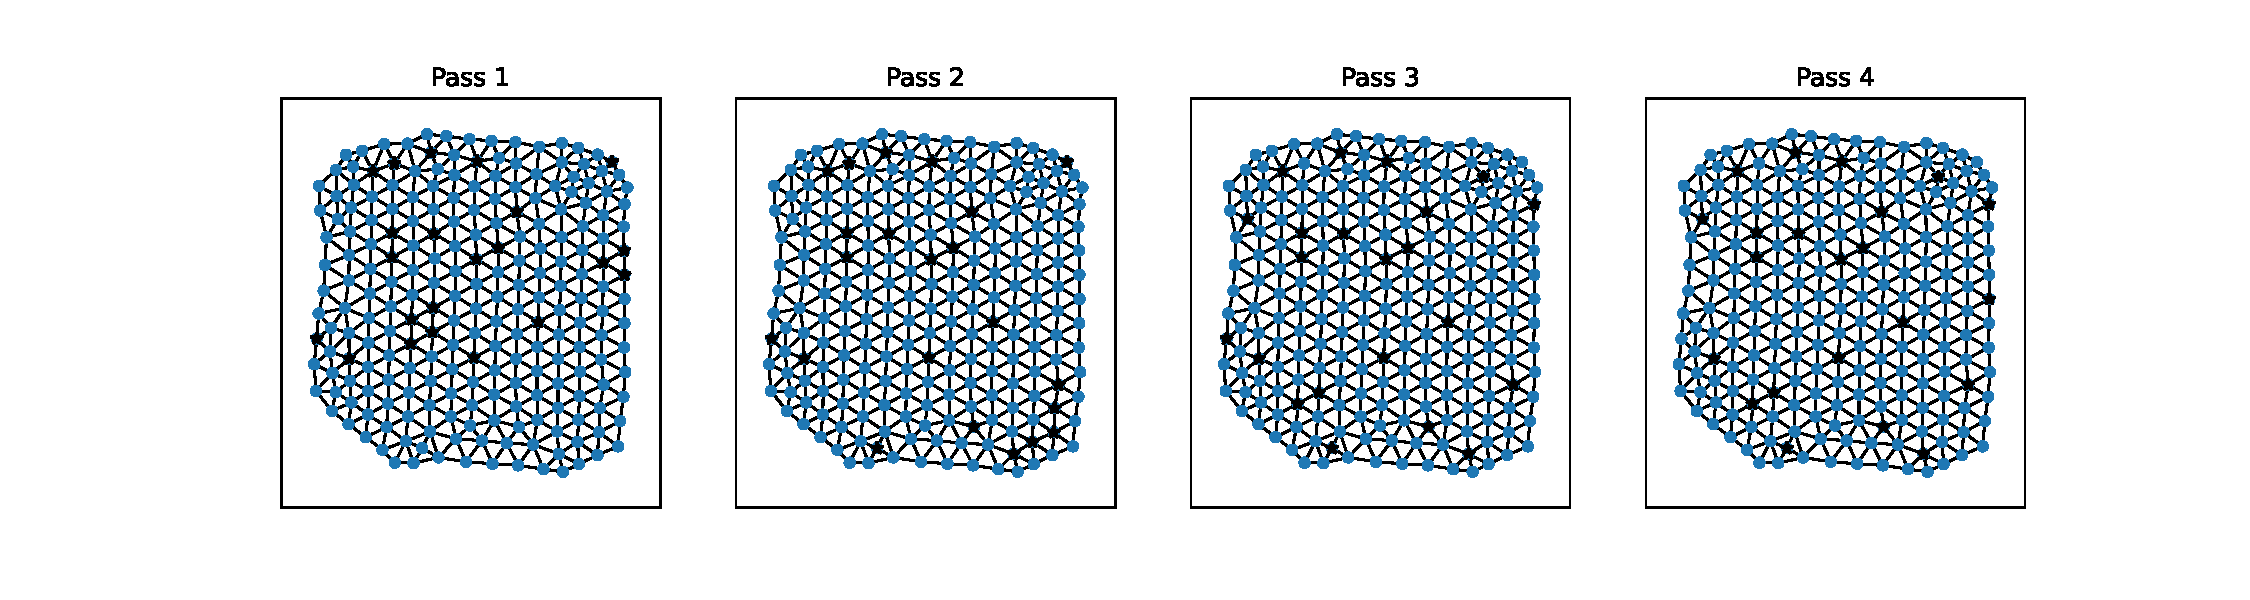
\includegraphics[width=\textwidth, trim=120 0 100 0, clip]{grid_700_agg_pass.pdf}
  \caption{Tentative aggregate centers after each binarization ``pass''.  This is the same mesh as in figure \ref{fig:grid700}.}
\end{figure}

\begin{figure}[h]
  \centering
  \begin{subfigure}[t]{0.32\textwidth}
    \centering
    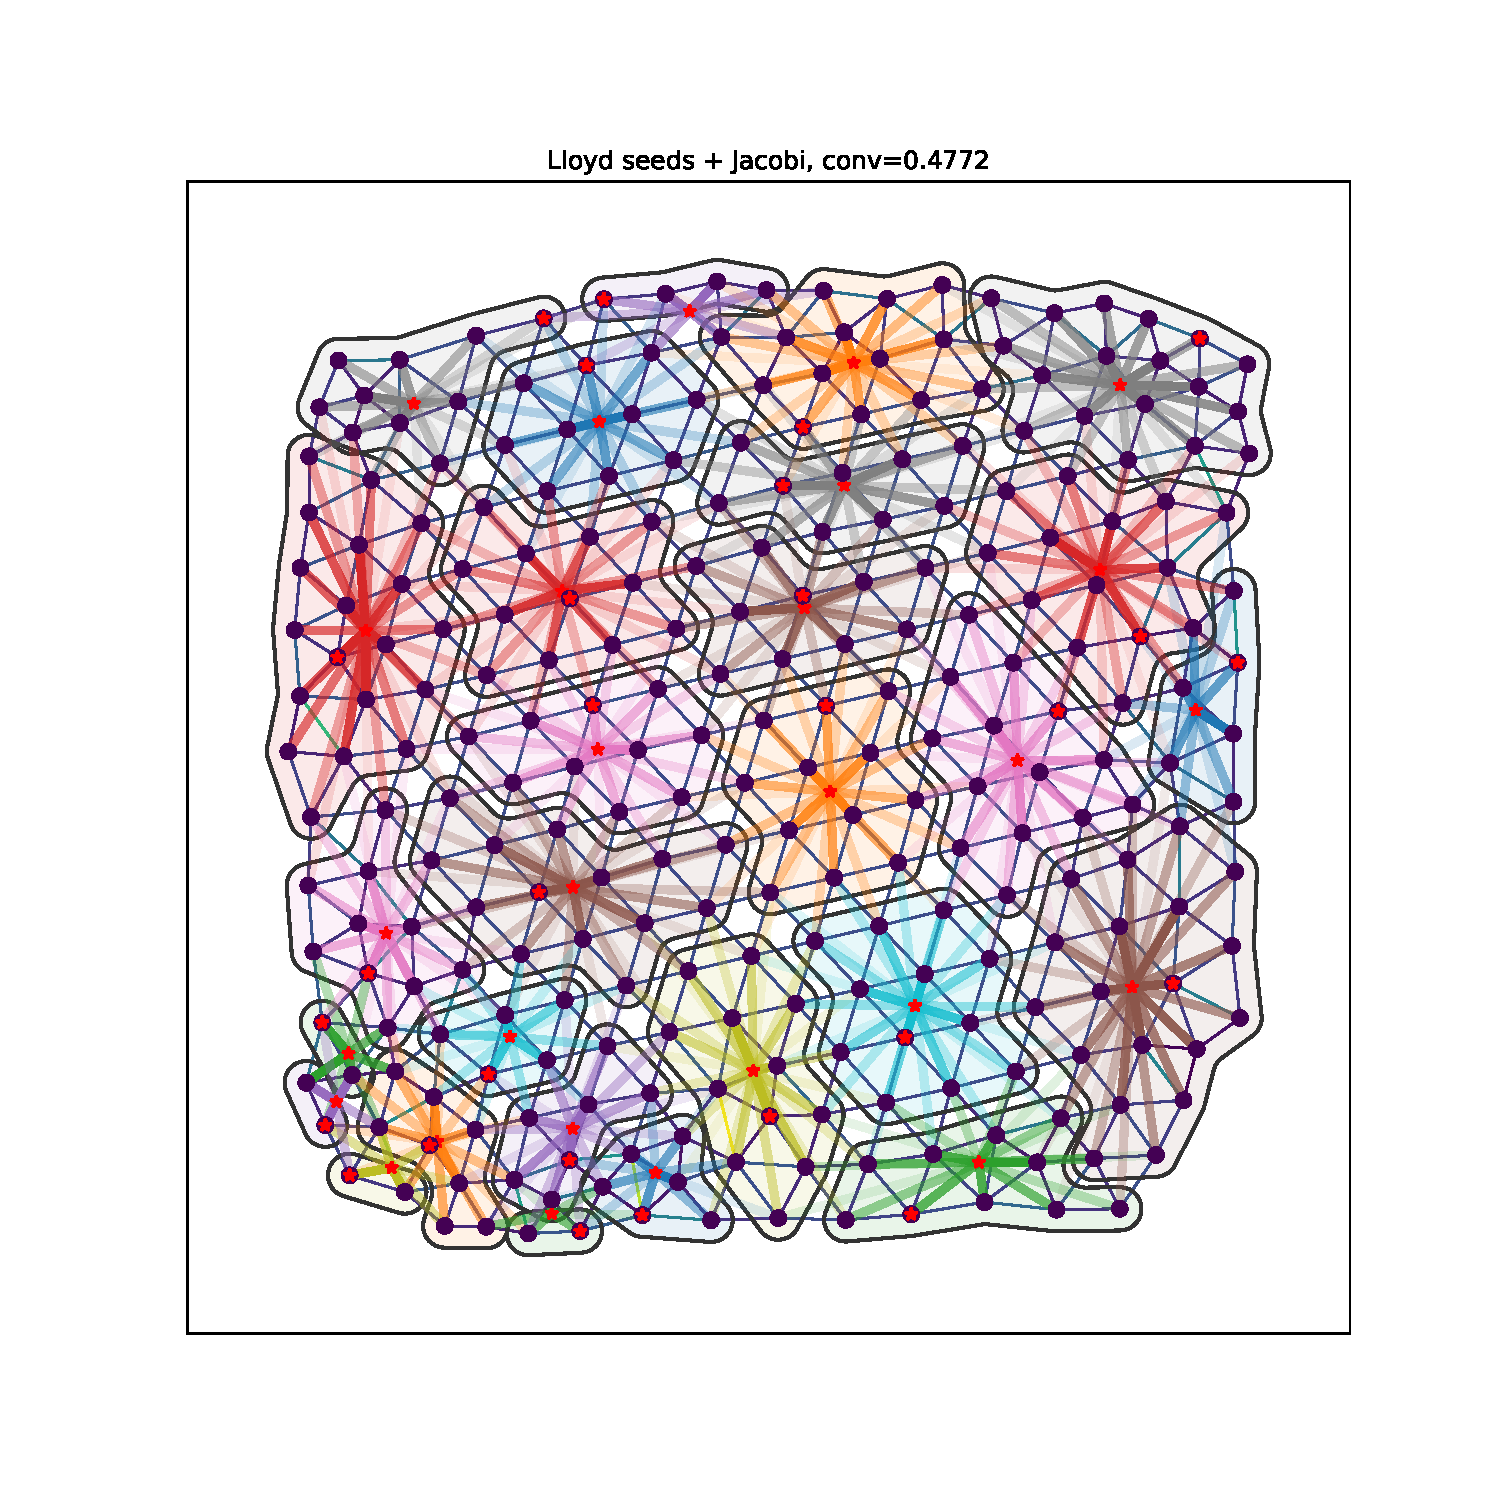
\includegraphics[width=\textwidth, trim=80 70 70 50, clip]{grid_800_dumb.pdf}
    \caption{Initial Lloyd Configuration}
  \end{subfigure}
  \begin{subfigure}[t]{0.32\textwidth}
    \centering
    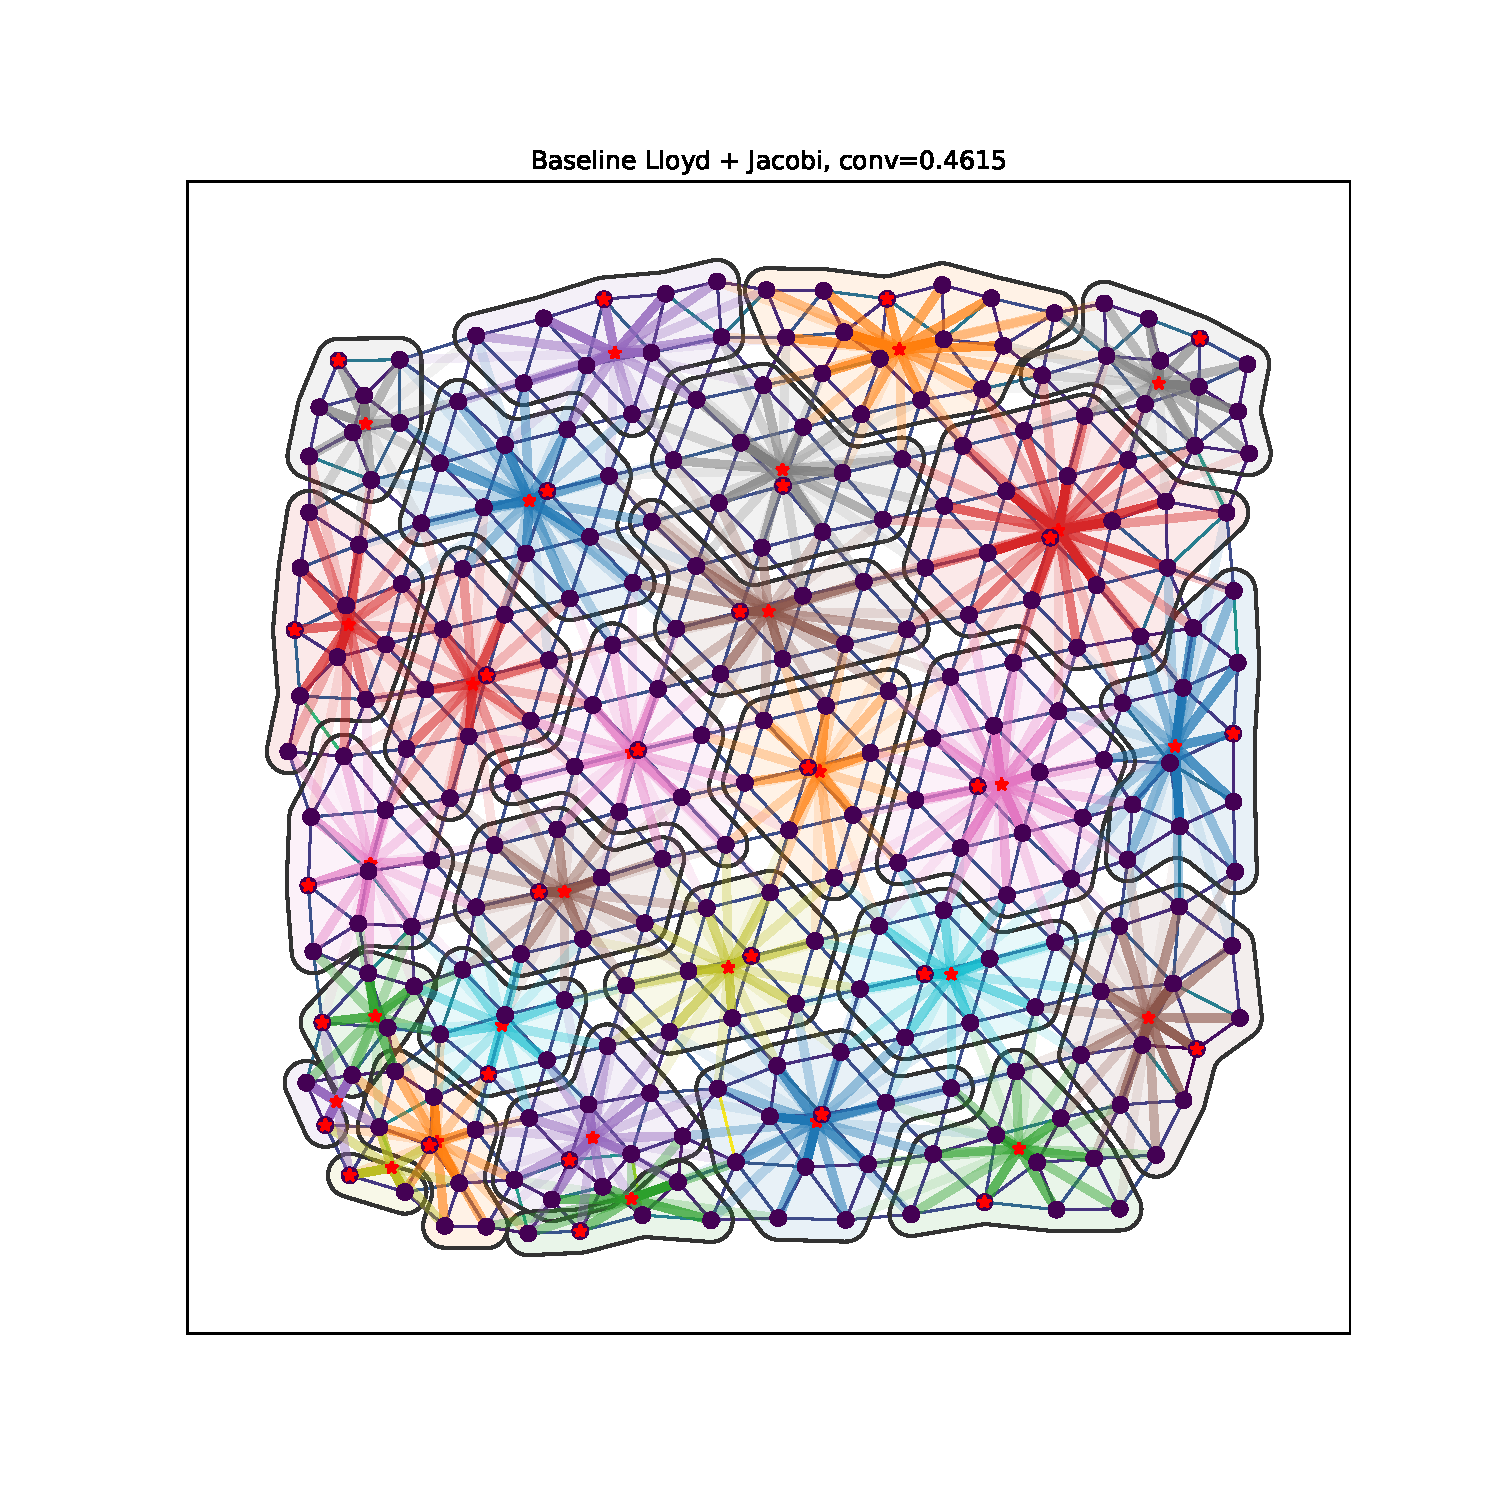
\includegraphics[width=\textwidth, trim=80 70 70 50, clip]{grid_800_lloyd.pdf}
    \caption{Lloyd + Jacobi}
  \end{subfigure}
  \begin{subfigure}[t]{0.32\textwidth}
    \centering
    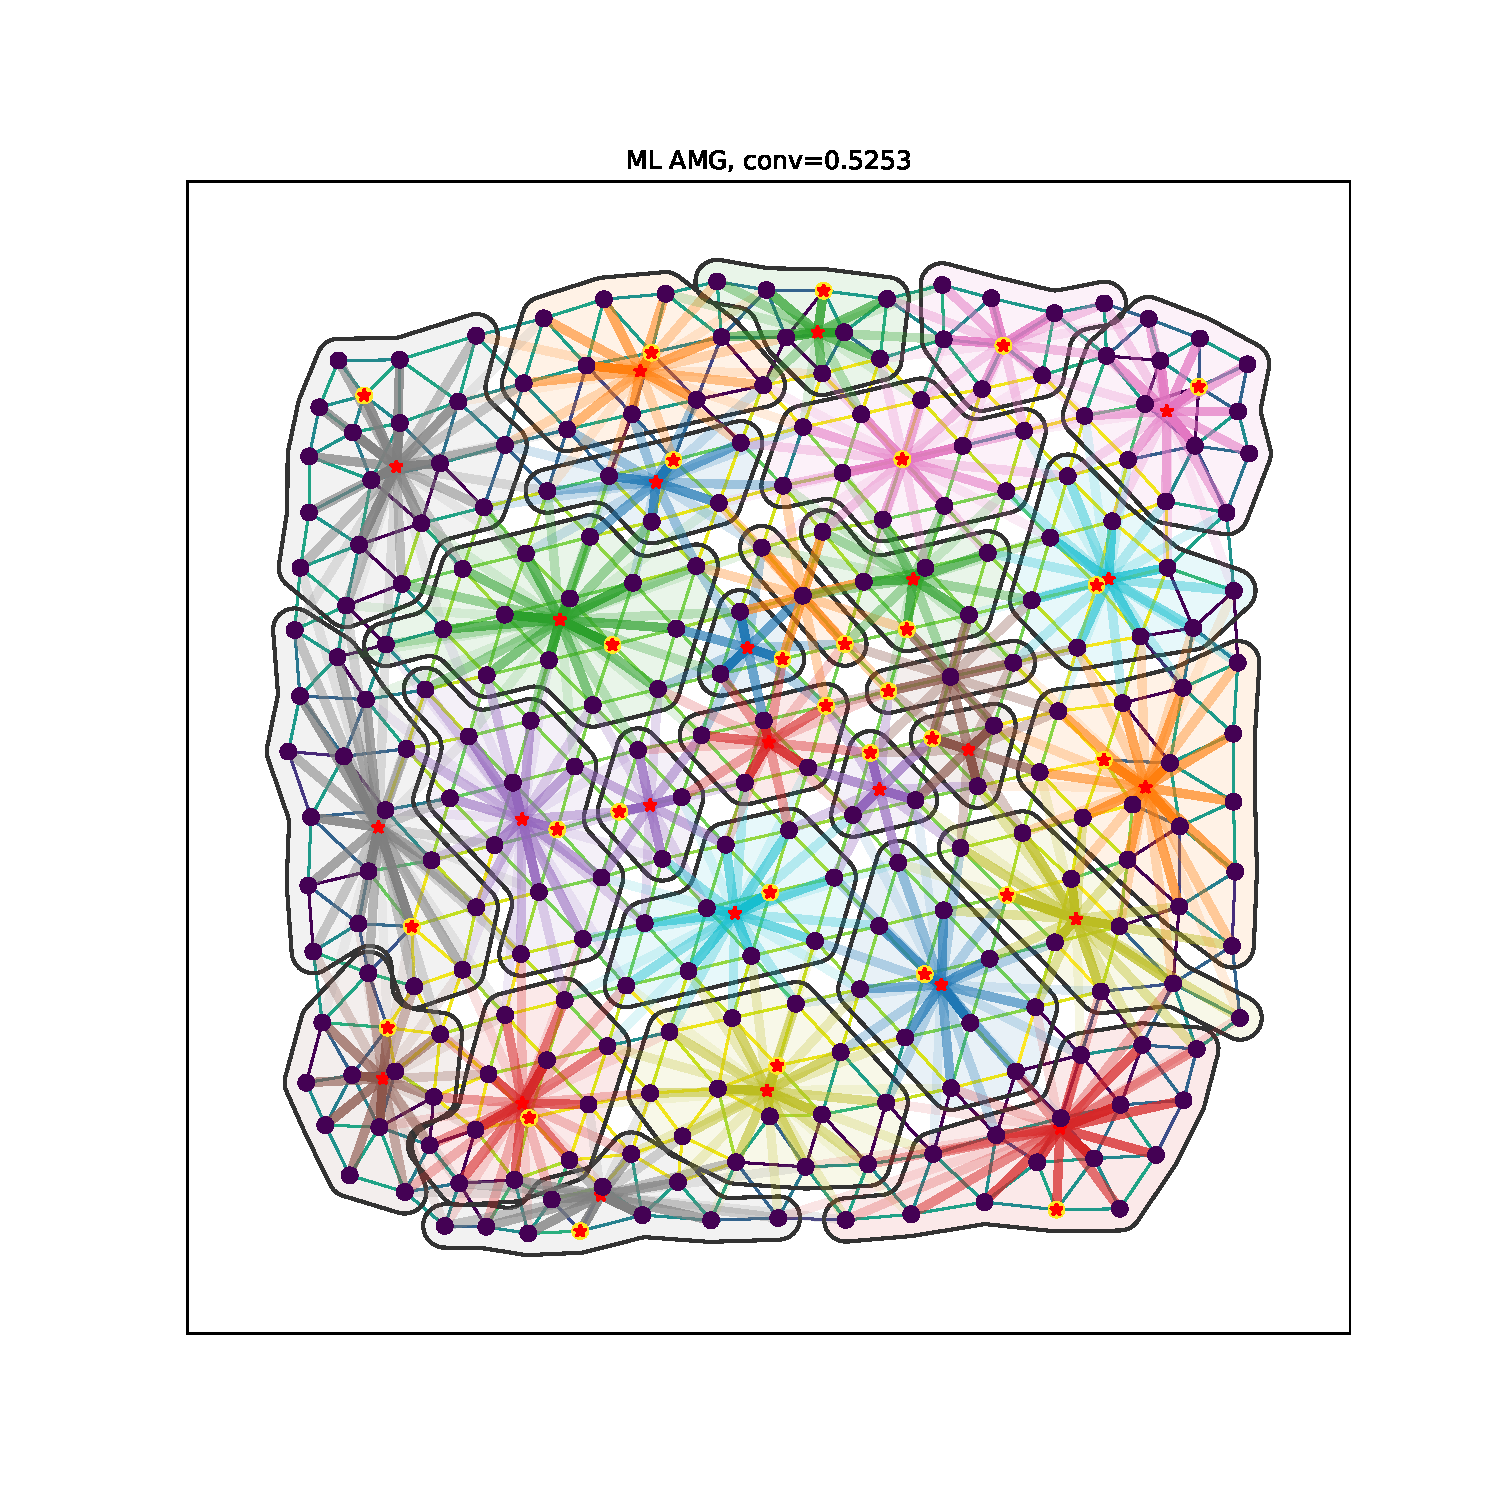
\includegraphics[width=\textwidth, trim=80 70 70 50, clip]{grid_800_ml.pdf}
    \caption{ML}
  \end{subfigure}
  \caption{Aggregate and interpolation data for a random unstructured mesh.  This particular mesh has 273 DoF.}
  \label{fig:grid800}
\end{figure}

\begin{figure}[h]
  \centering
  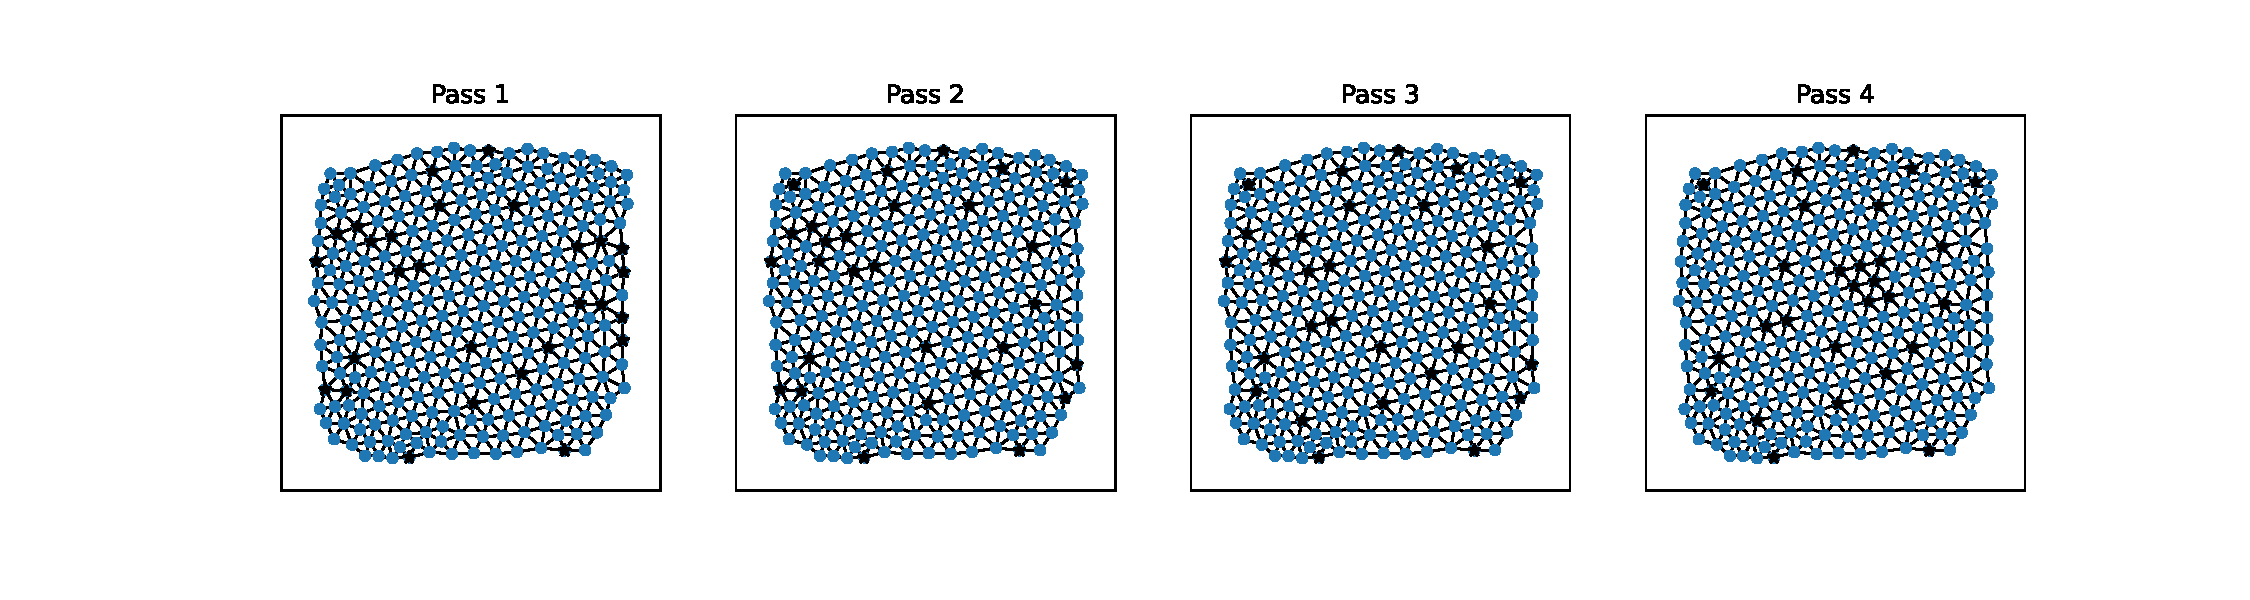
\includegraphics[width=\textwidth, trim=120 0 100 0, clip]{grid_800_agg_pass.pdf}
  \caption{Tentative aggregate centers after each binarization ``pass''.  This is the same mesh as in figure \ref{fig:grid800}.}
\end{figure}

\begin{figure}[h]
  \centering
  \begin{subfigure}[t]{0.32\textwidth}
    \centering
    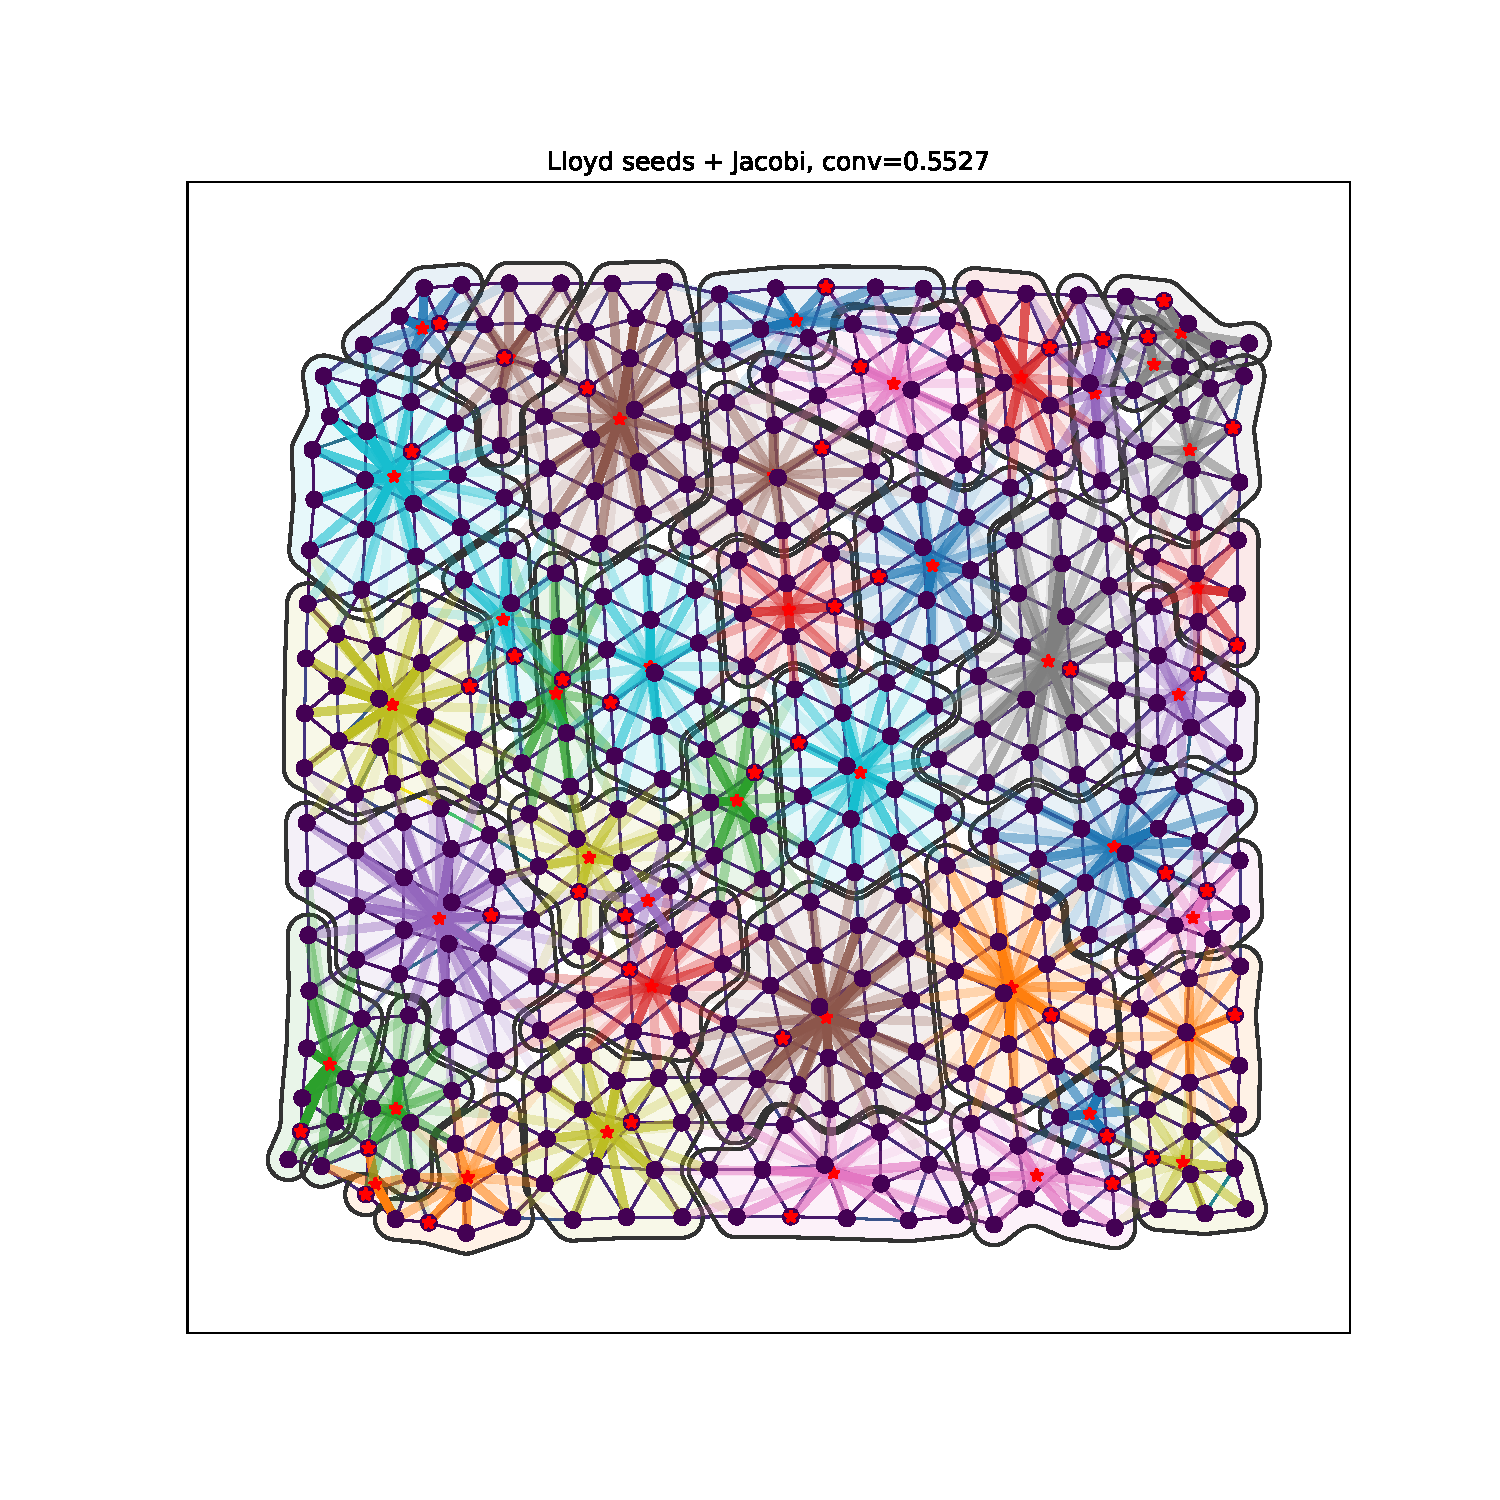
\includegraphics[width=\textwidth, trim=80 70 70 50, clip]{grid_largest_dumb.pdf}
    \caption{Initial Lloyd Configuration}
  \end{subfigure}
  \begin{subfigure}[t]{0.32\textwidth}
    \centering
    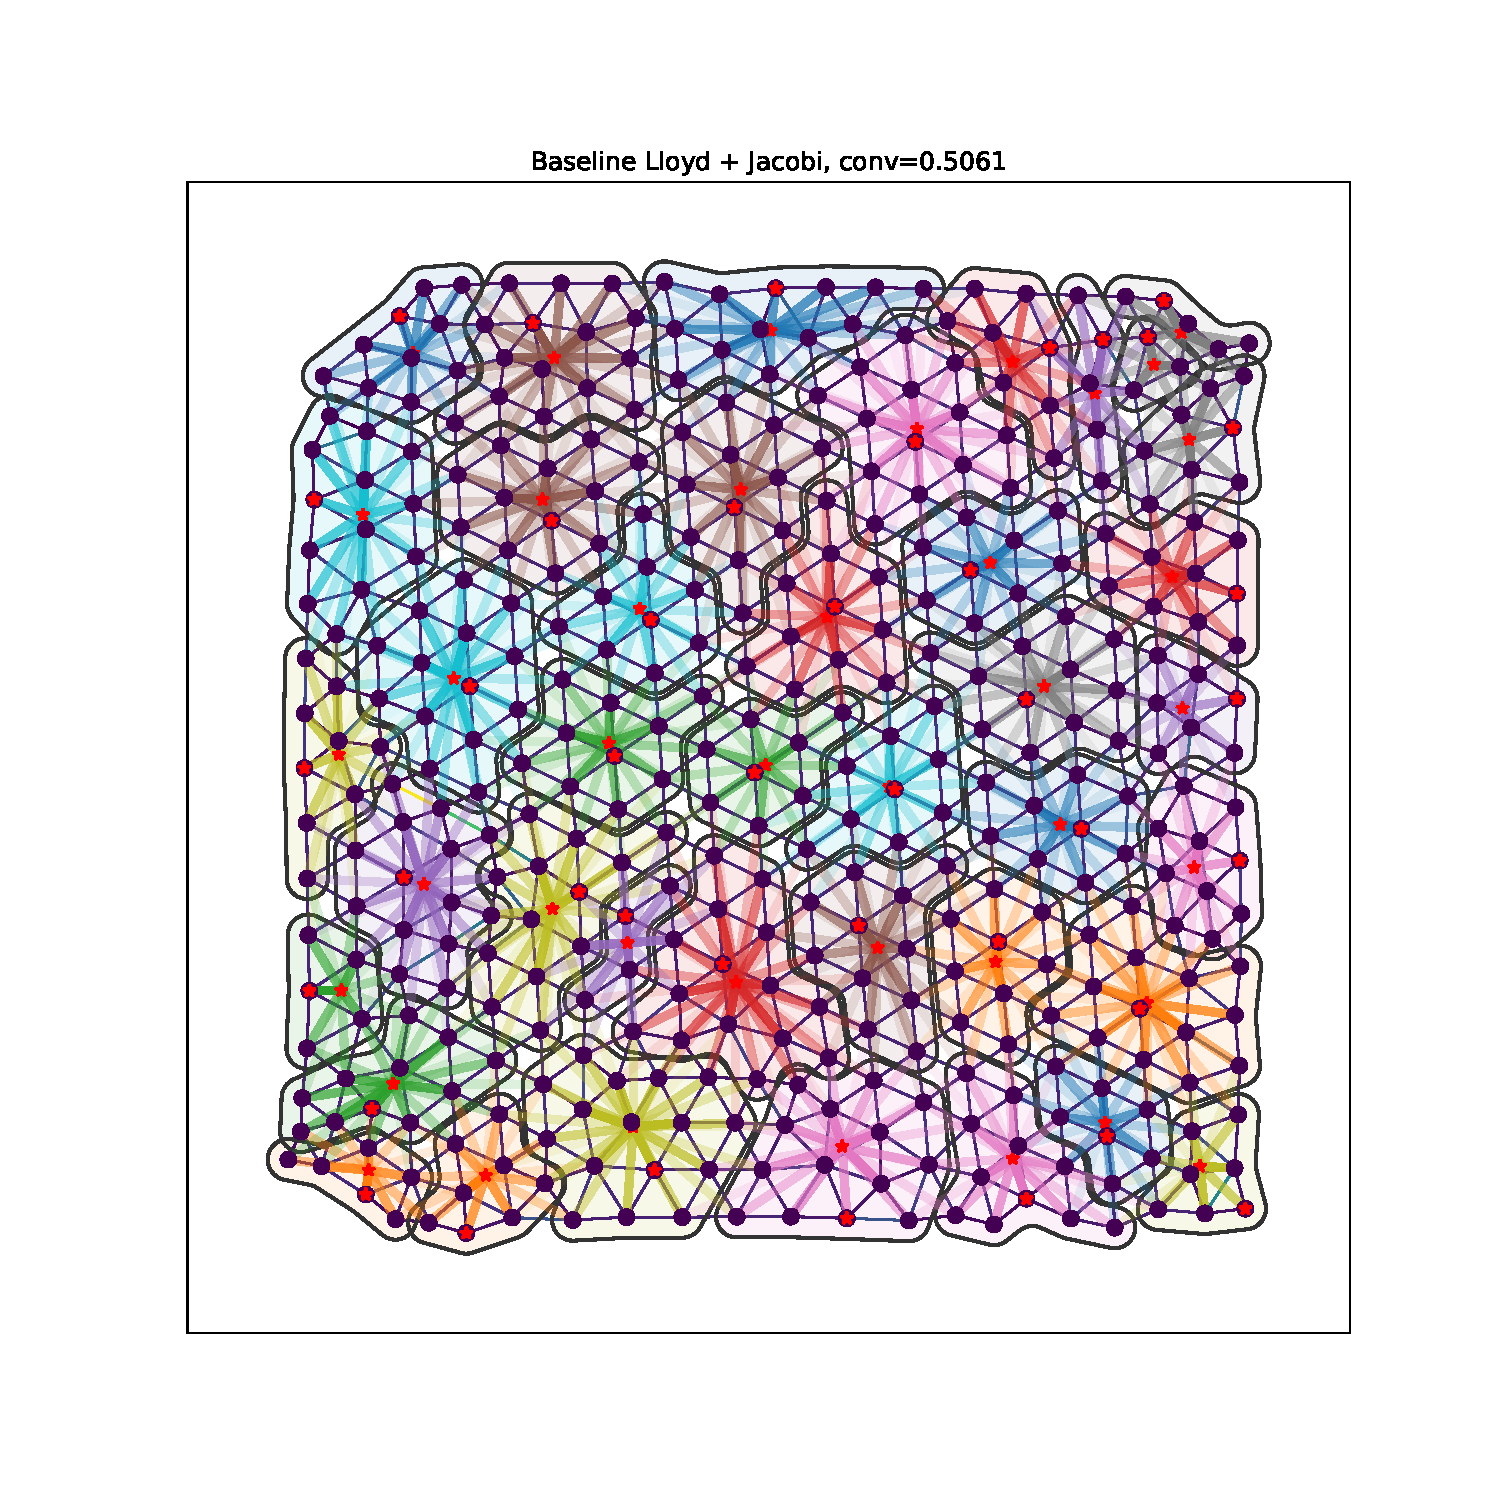
\includegraphics[width=\textwidth, trim=80 70 70 50, clip]{grid_largest_lloyd.pdf}
    \caption{Lloyd + Jacobi}
  \end{subfigure}
  \begin{subfigure}[t]{0.32\textwidth}
    \centering
    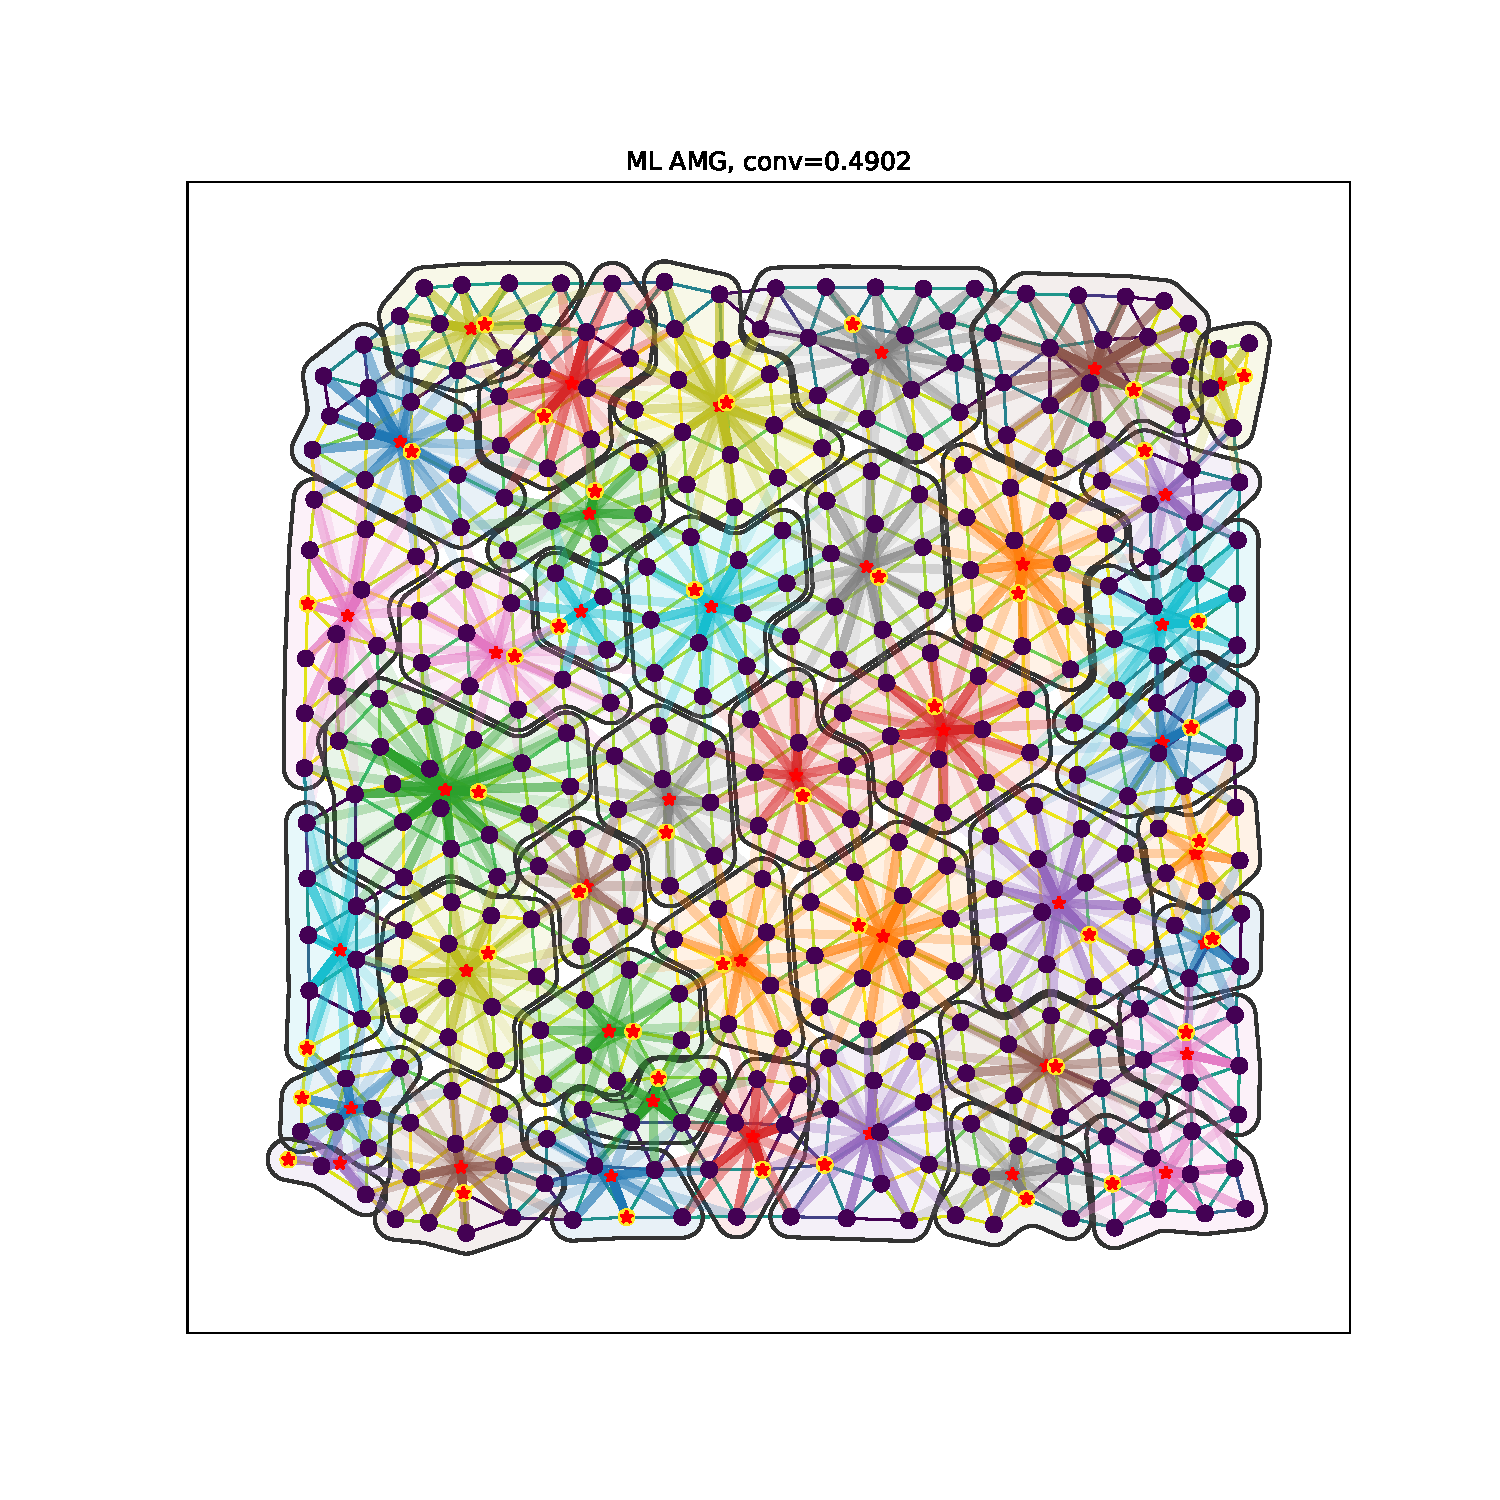
\includegraphics[width=\textwidth, trim=80 70 70 50, clip]{grid_largest_ml.pdf}
    \caption{ML}
  \end{subfigure}
  \caption{Aggregate and interpolation data for the largest mesh in the \textit{training set}.  This particular mesh has 410 DoF.}
  \label{fig:gridlargest}
\end{figure}

\begin{figure}[h]
  \centering
  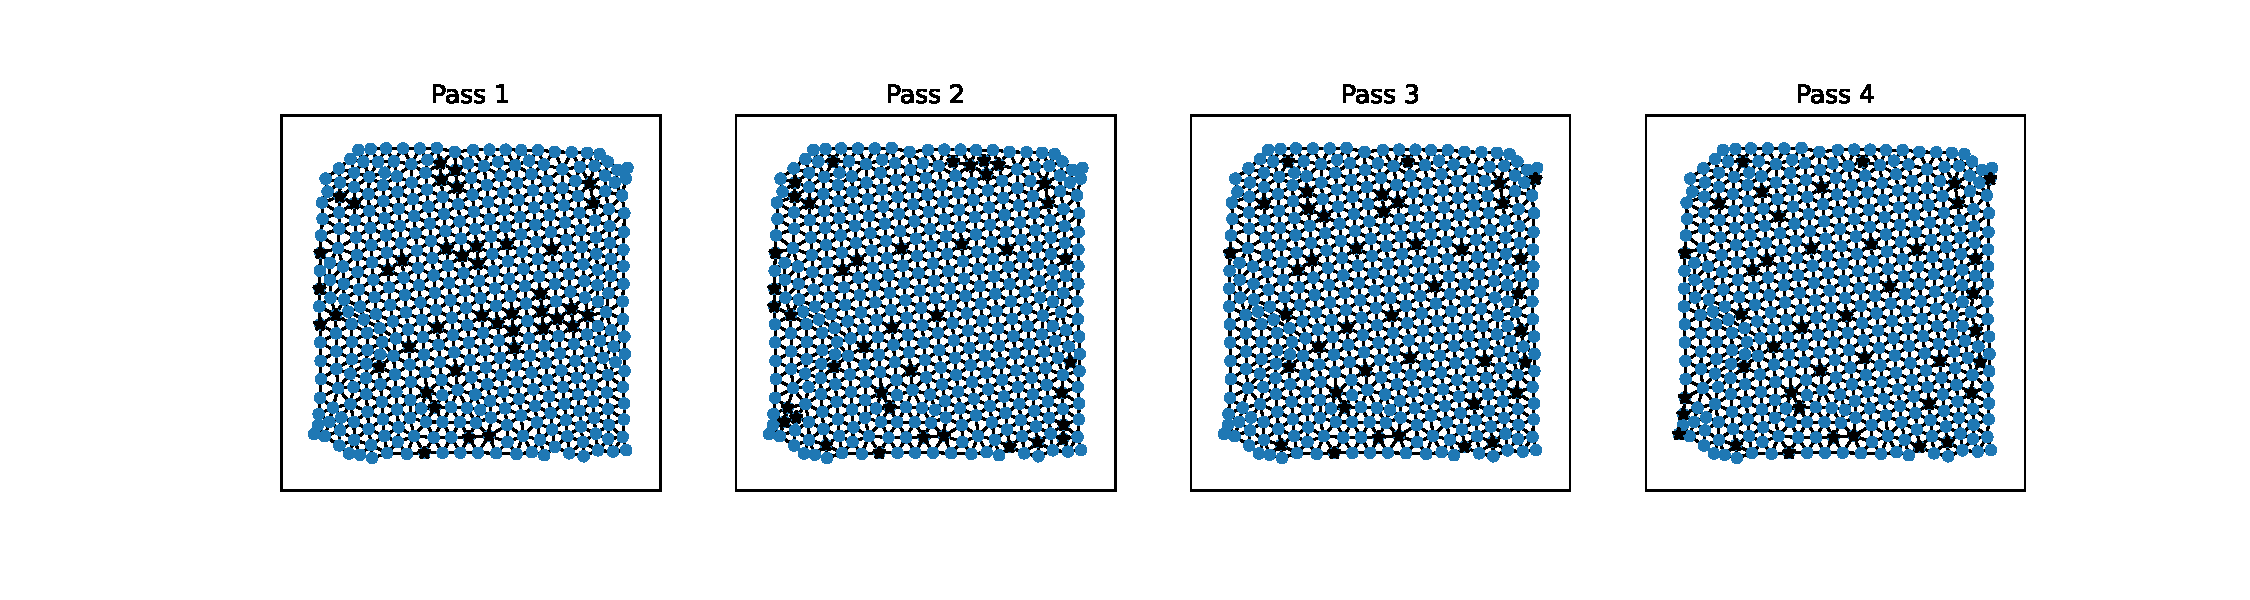
\includegraphics[width=\textwidth, trim=120 0 100 0, clip]{grid_largest_agg_pass.pdf}
  \caption{Tentative aggregate centers after each binarization ``pass''.  This is the same mesh as in figure \ref{fig:gridlargest}.}
\end{figure}

\FloatBarrier
\subsection{Anisotropic Results}

\begin{figure}[h]
  \centering
  \begin{subfigure}[t]{0.49\textwidth}
    \centering
    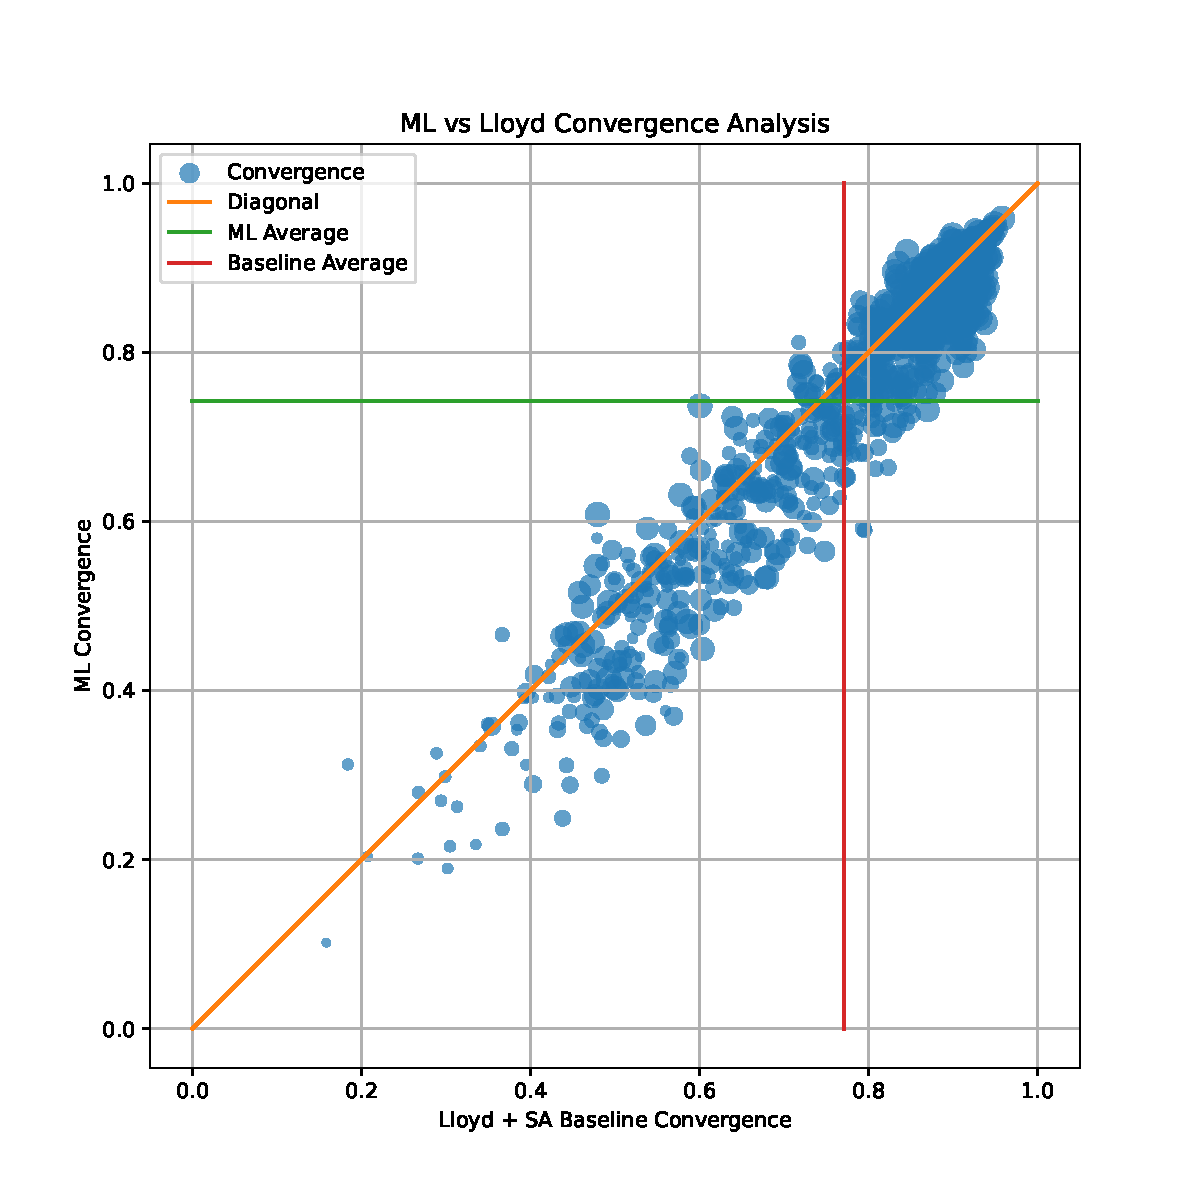
\includegraphics[width=\textwidth]{aniso_train_convergence.pdf}
    \caption{Training convergence}
  \end{subfigure}
  \begin{subfigure}[t]{0.49\textwidth}
    \centering
    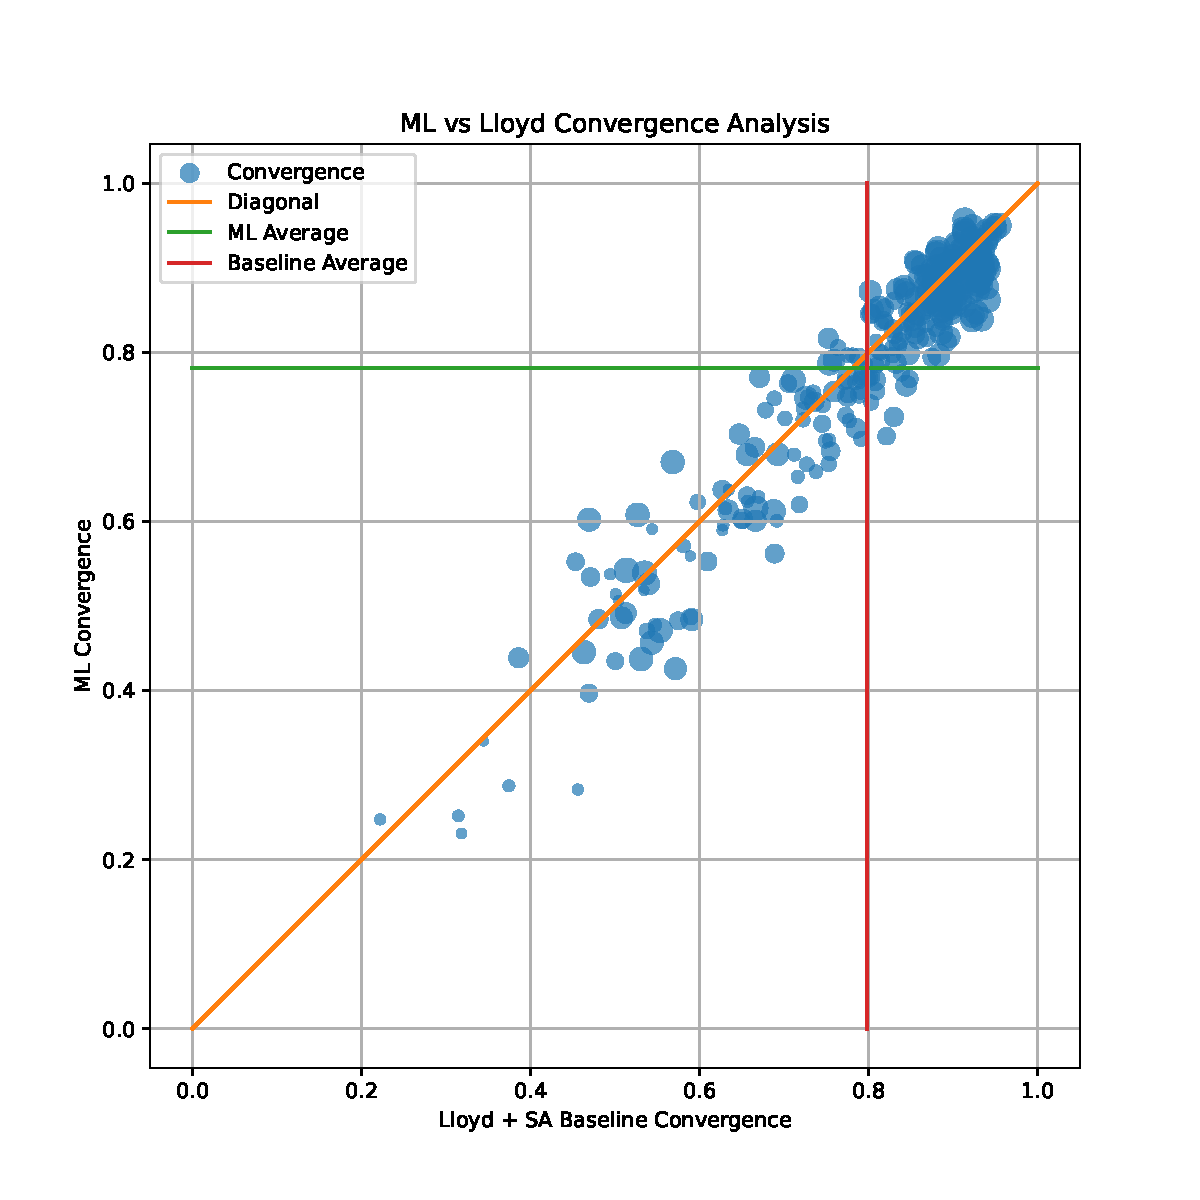
\includegraphics[width=\textwidth]{aniso_test_convergence.pdf}
    \caption{Testing convergence}
  \end{subfigure}
  \caption{Convergence data for the ML AMG method vs a baseline Lloyd and Jacobi SA method.  Values below the diagonal indicate a better convergence for the ML.  Markers are scaled by problem size.}
  \label{fig:aniso_conv}
\end{figure}

\begin{figure}[h]
  \centering
  \begin{subfigure}[t]{0.49\textwidth}
    \centering
    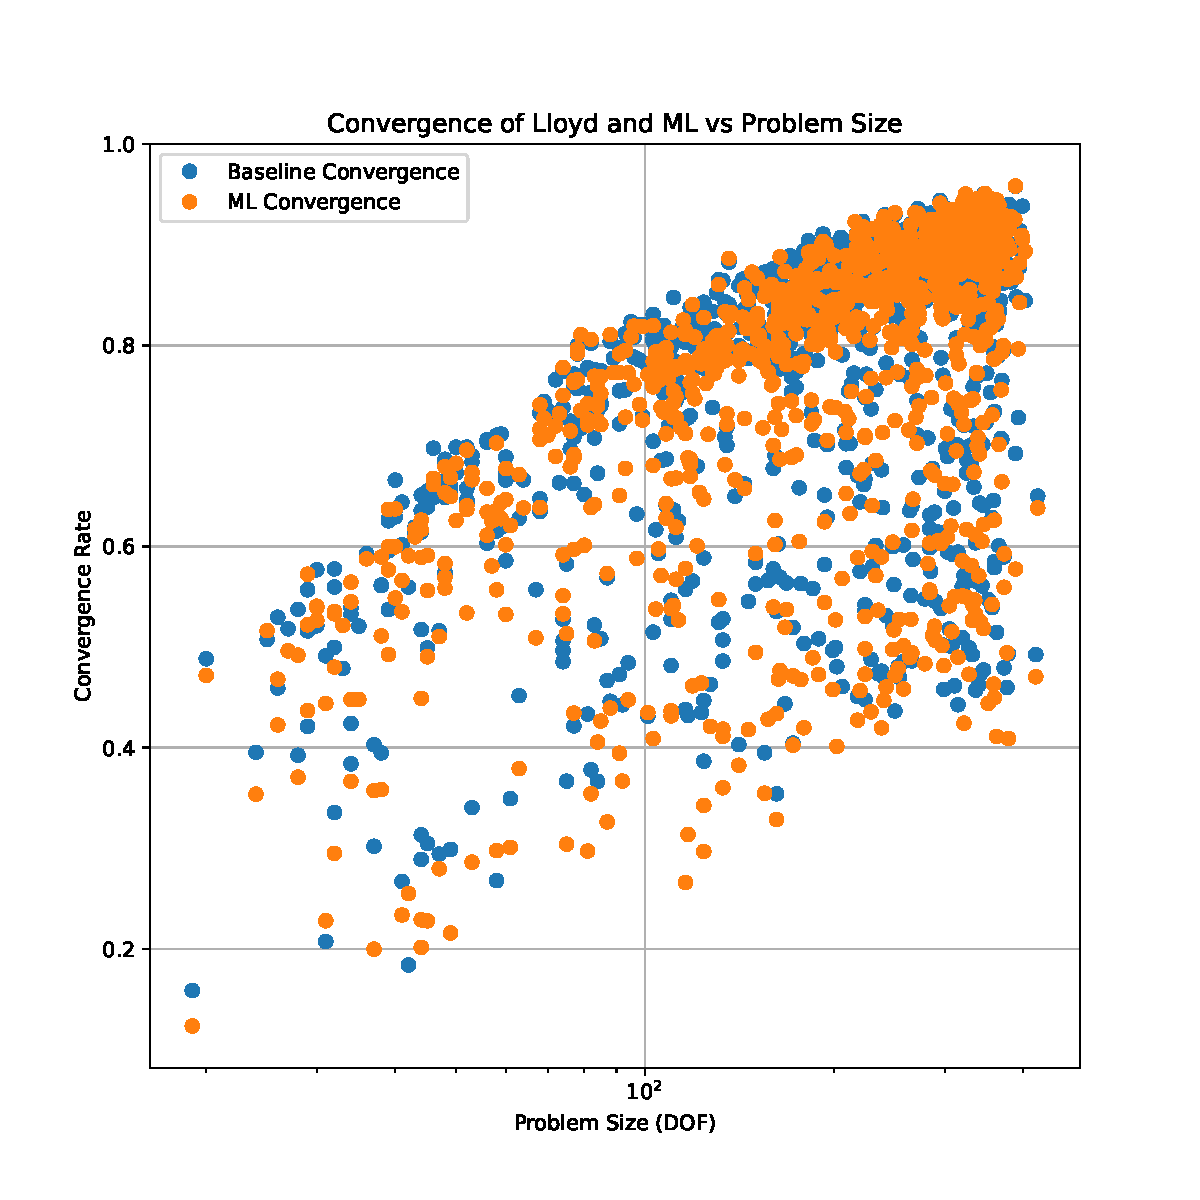
\includegraphics[width=\textwidth]{aniso_train_convergence_per_size.pdf}
    \caption{Training convergence}
  \end{subfigure}
  \begin{subfigure}[t]{0.49\textwidth}
    \centering
    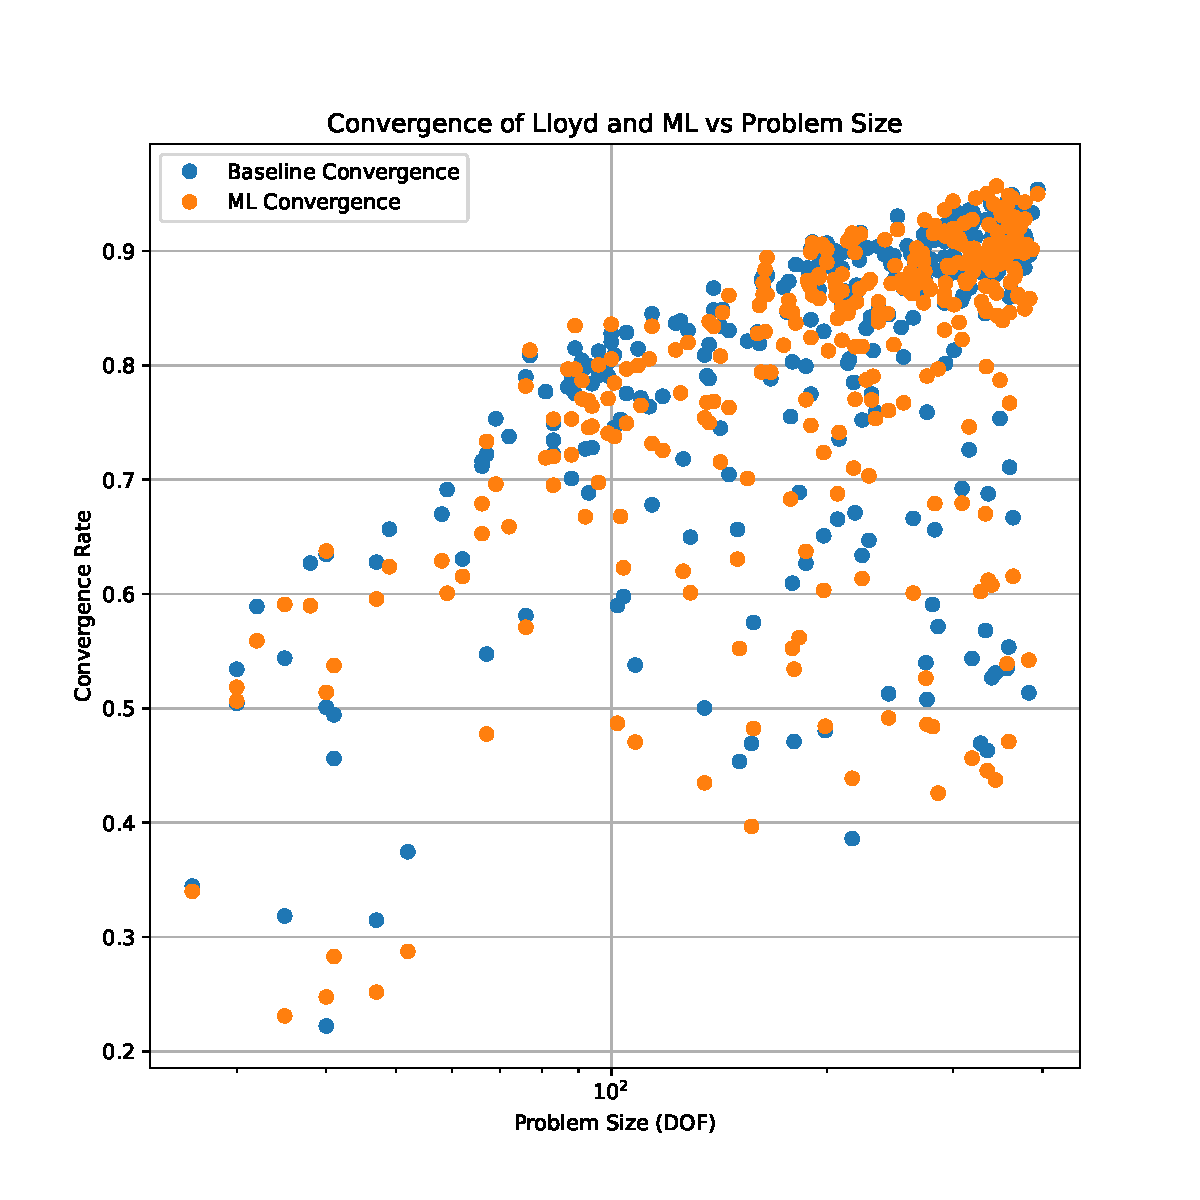
\includegraphics[width=\textwidth]{aniso_test_convergence_per_size.pdf}
    \caption{Testing convergence}
  \end{subfigure}
  \caption{Convergence data for the two methods plotted against problem size (DOF).  The ML method seems biased towards better performance on the smaller problems, and does not do as well on the larger problems.}
  \label{fig:aniso_conv_per_size}
\end{figure}

\begin{figure}[h]
  \centering
  \begin{subfigure}[t]{0.49\textwidth}
    \centering
    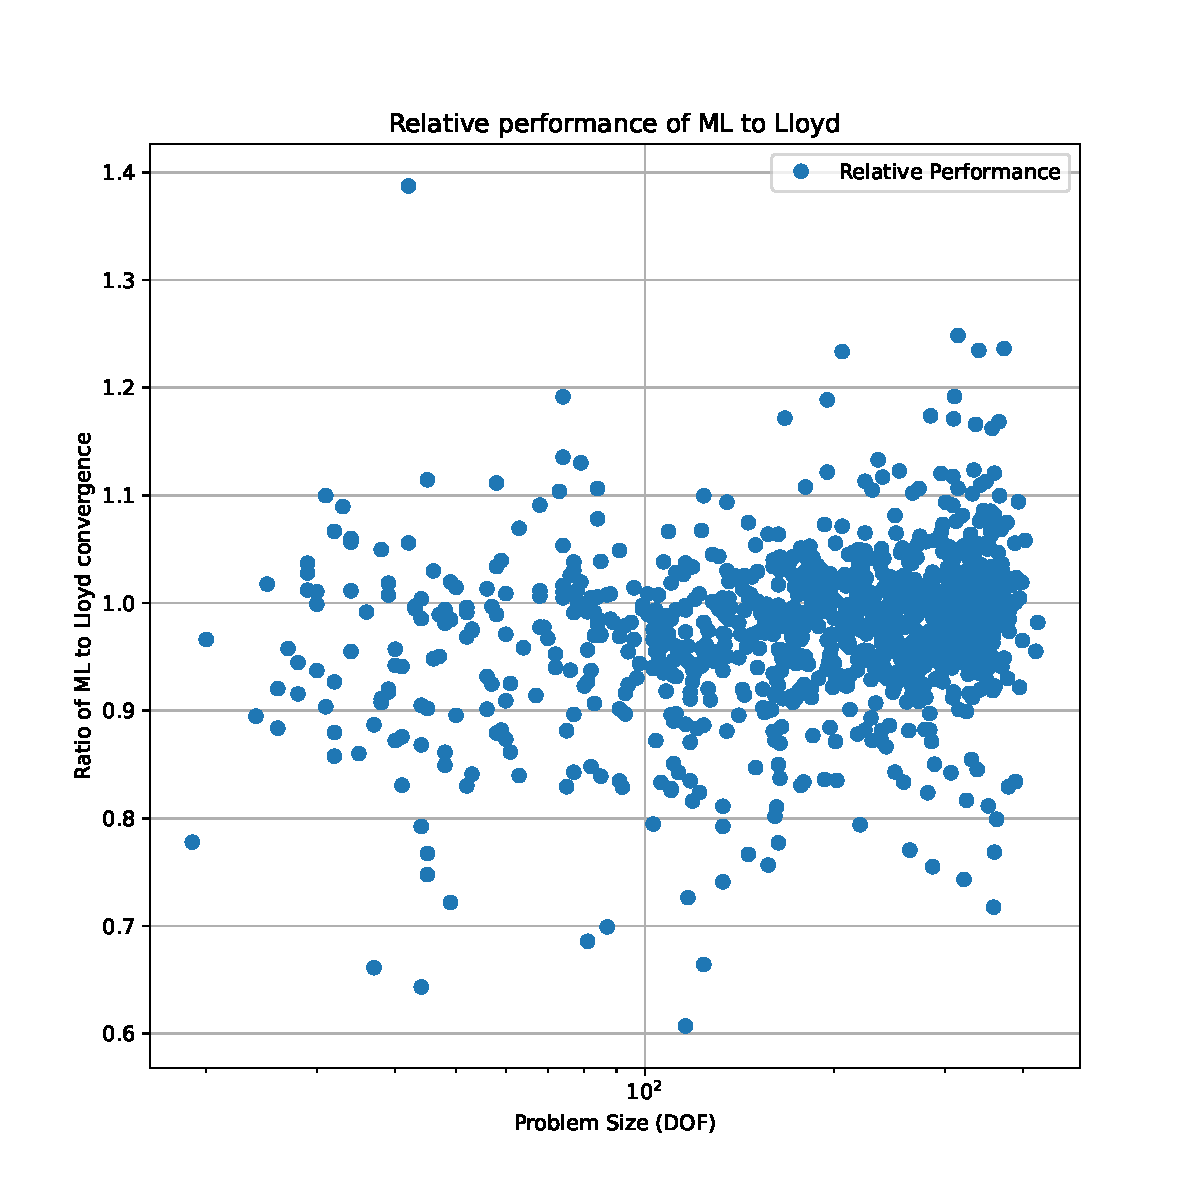
\includegraphics[width=\textwidth]{aniso_rel_perf_train.pdf}
    \caption{Relative training performance}
  \end{subfigure}
  \begin{subfigure}[t]{0.49\textwidth}
    \centering
    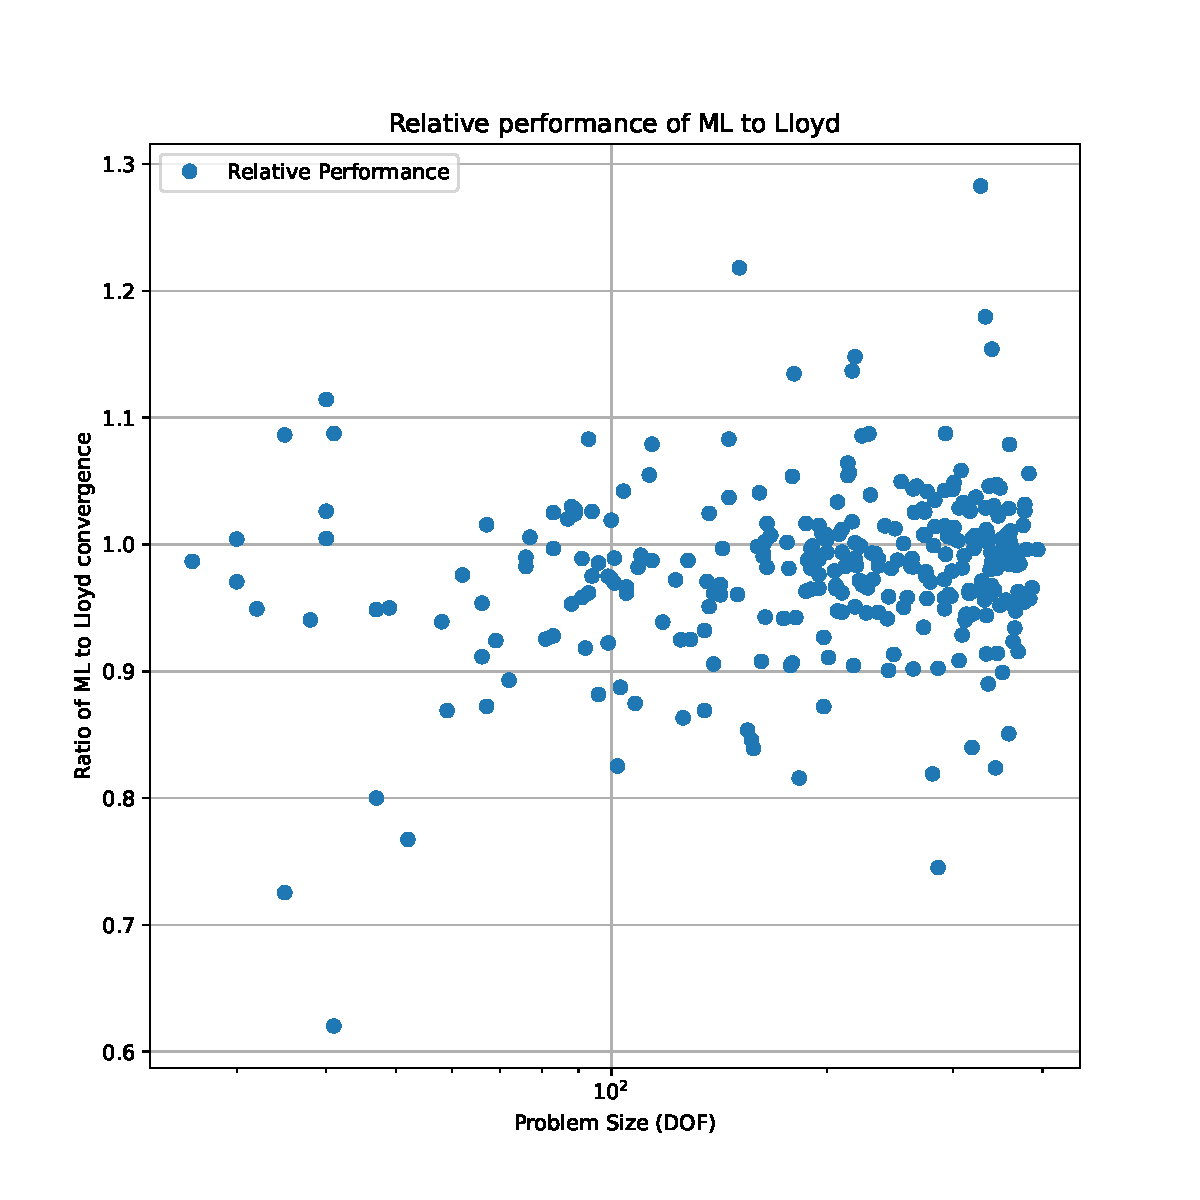
\includegraphics[width=\textwidth]{aniso_rel_perf_test.pdf}
    \caption{Relative testing performance}
  \end{subfigure}
  \caption{Relative performance of the ML to the Lloyd method, plotted against problem size.  Relative performance is obtained by dividing the ML convergence by the Lloyd convergence for each problem.  Values below $1$ indicate better ML performance, while values above $1$ indicate better baseline performance.}
  \label{fig:aniso_rel_conv}
\end{figure}

\begin{figure}[h]
  \centering
  \begin{subfigure}[t]{0.32\textwidth}
    \centering
    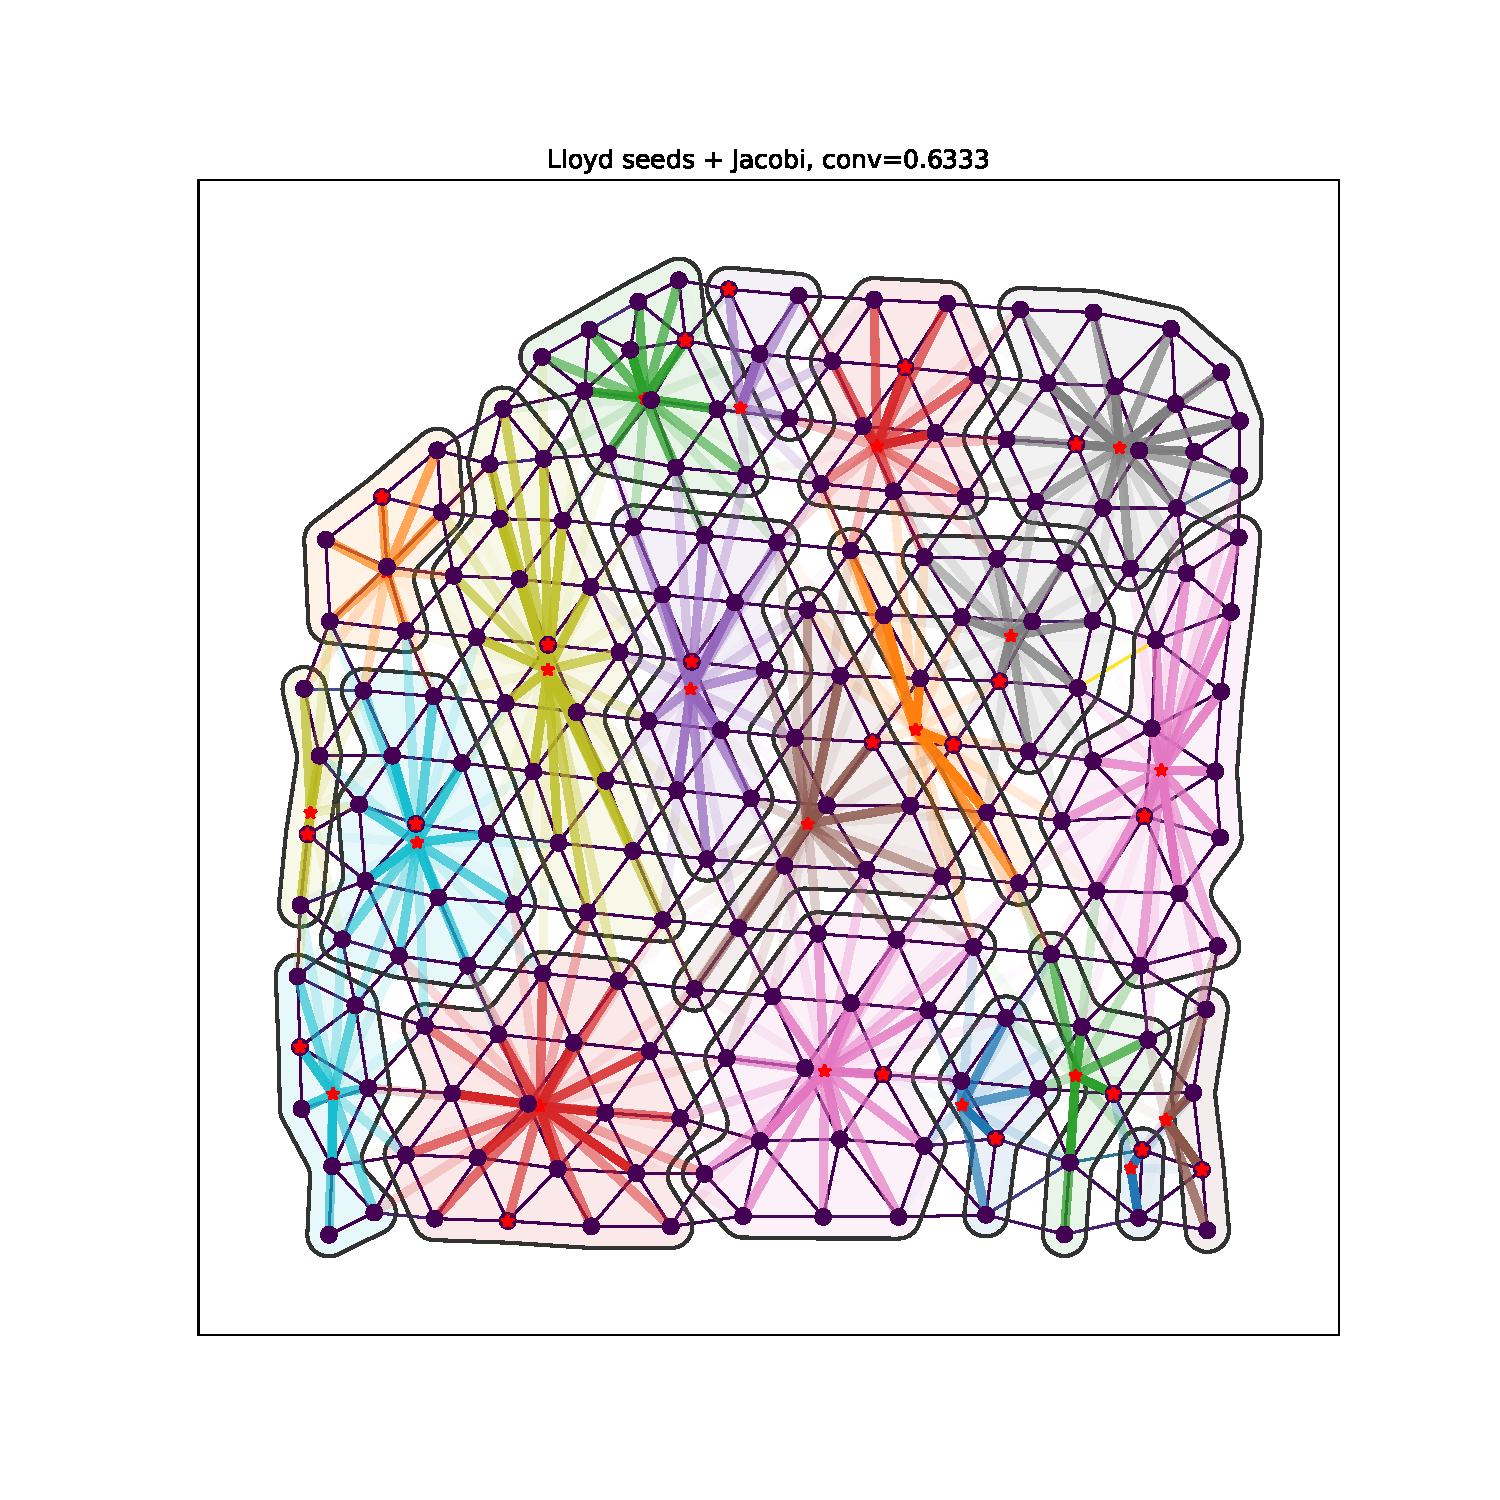
\includegraphics[width=\textwidth, trim=80 70 70 50, clip]{grid_anis_3_dumb.pdf}
    \caption{Initial Lloyd Configuration}
  \end{subfigure}
  \begin{subfigure}[t]{0.32\textwidth}
    \centering
    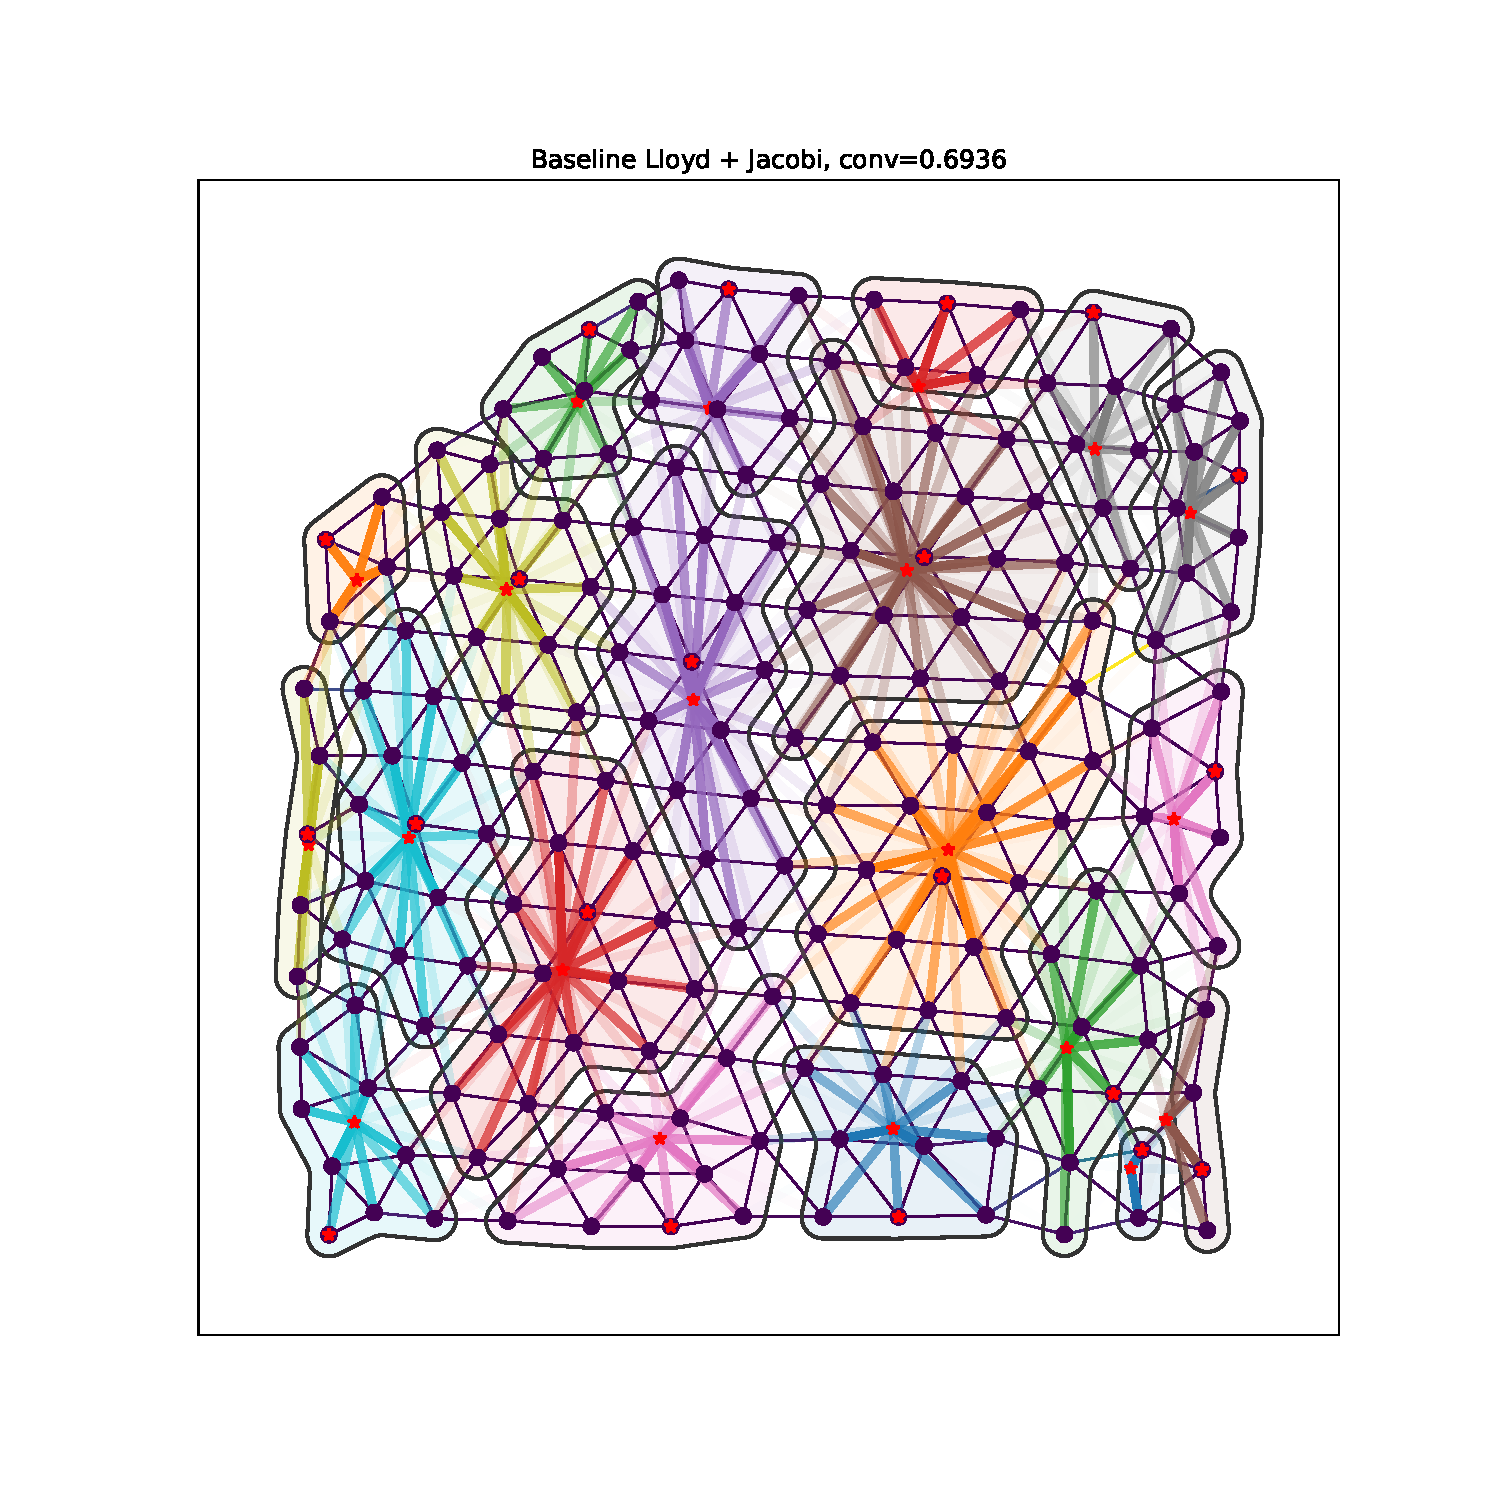
\includegraphics[width=\textwidth, trim=80 70 70 50, clip]{grid_anis_3_lloyd.pdf}
    \caption{Lloyd + Jacobi}
  \end{subfigure}
  \begin{subfigure}[t]{0.32\textwidth}
    \centering
    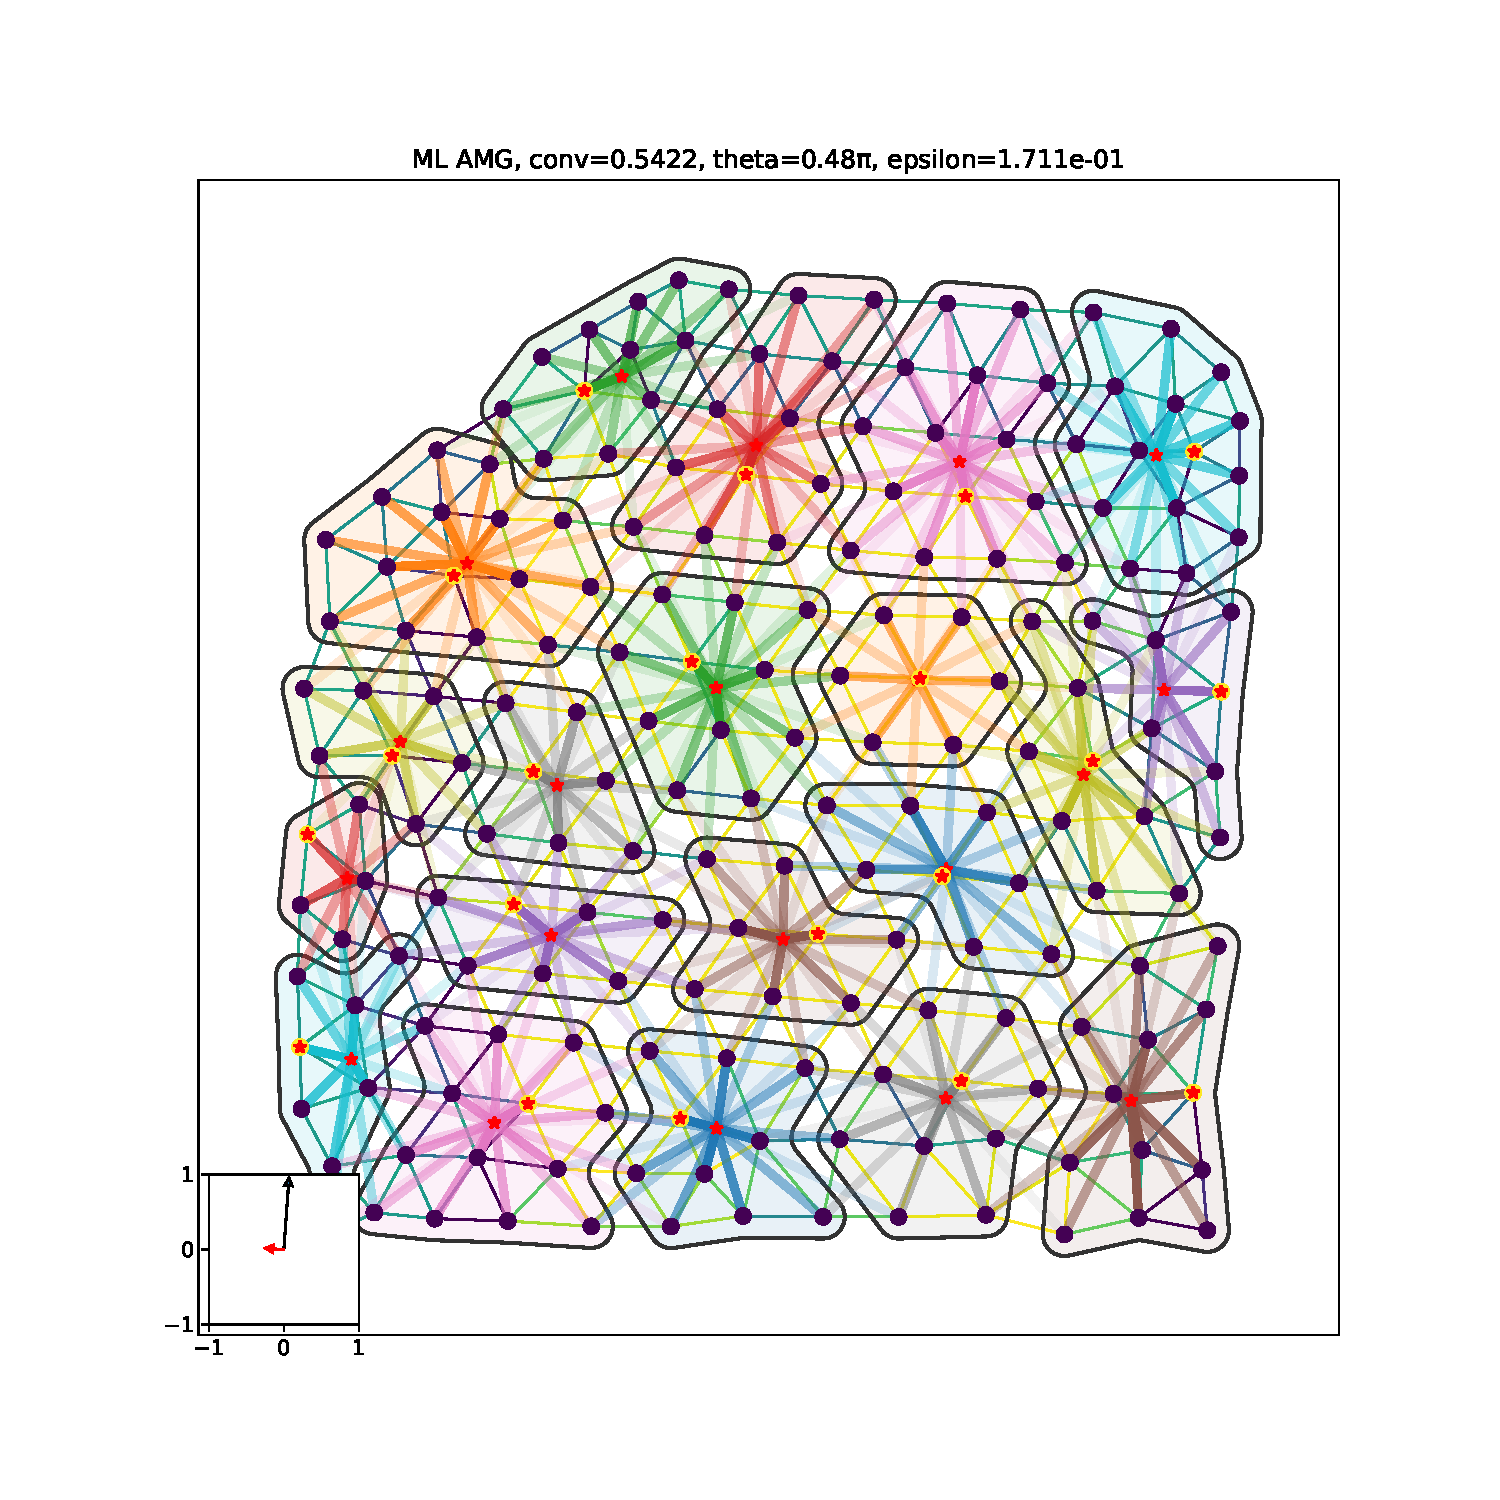
\includegraphics[width=\textwidth, trim=80 70 70 50, clip]{grid_anis_3_ml.pdf}
    \caption{ML}
  \end{subfigure}
  \caption{Aggregate and interpolation data for a random anisotropic mesh.  This is a different network from the isotropic case.}
  \label{fig:grid_anis_3}
\end{figure}

\begin{figure}[h]
  \centering
  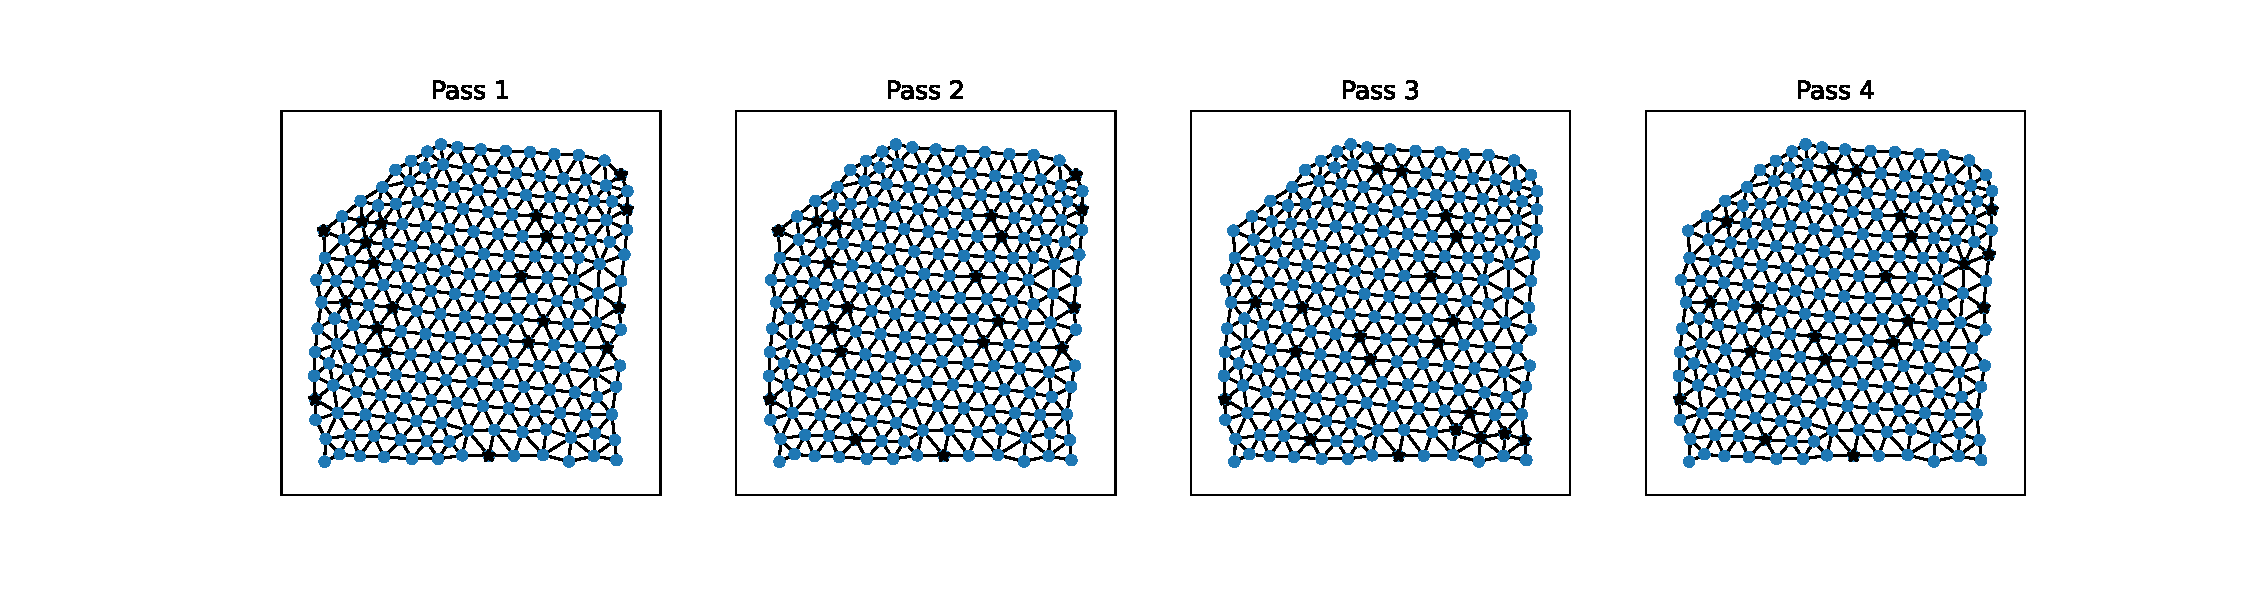
\includegraphics[width=\textwidth, trim=120 0 100 0, clip]{grid_anis_3_agg_pass.pdf}
  \caption{Tentative aggregate centers after each binarization ``pass''.  This is the same mesh as in figure \ref{fig:grid_anis_3}.}
\end{figure}

\begin{figure}[h]
  \centering
  \begin{subfigure}[t]{0.32\textwidth}
    \centering
    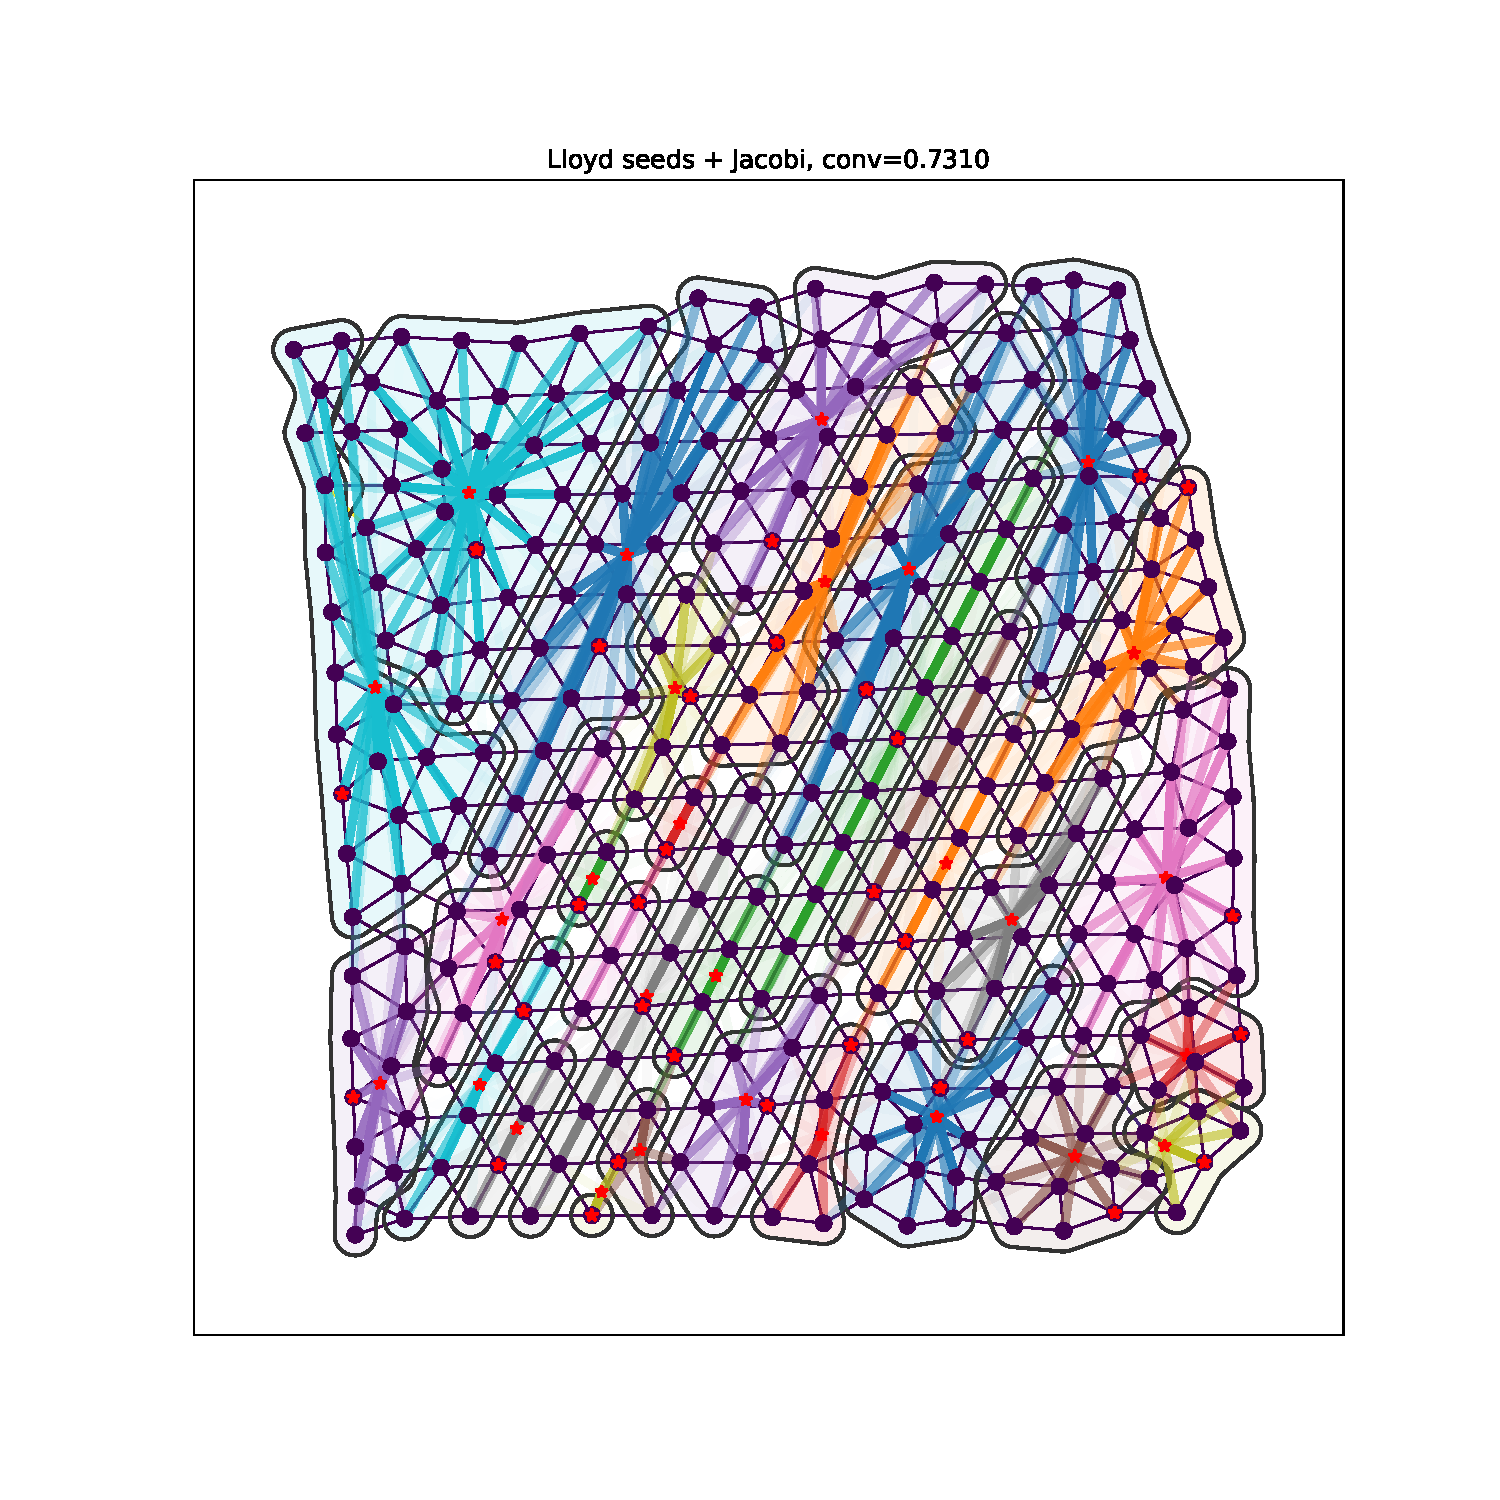
\includegraphics[width=\textwidth, trim=80 70 70 50, clip]{grid_anis_4_dumb.pdf}
    \caption{Initial Lloyd Configuration}
  \end{subfigure}
  \begin{subfigure}[t]{0.32\textwidth}
    \centering
    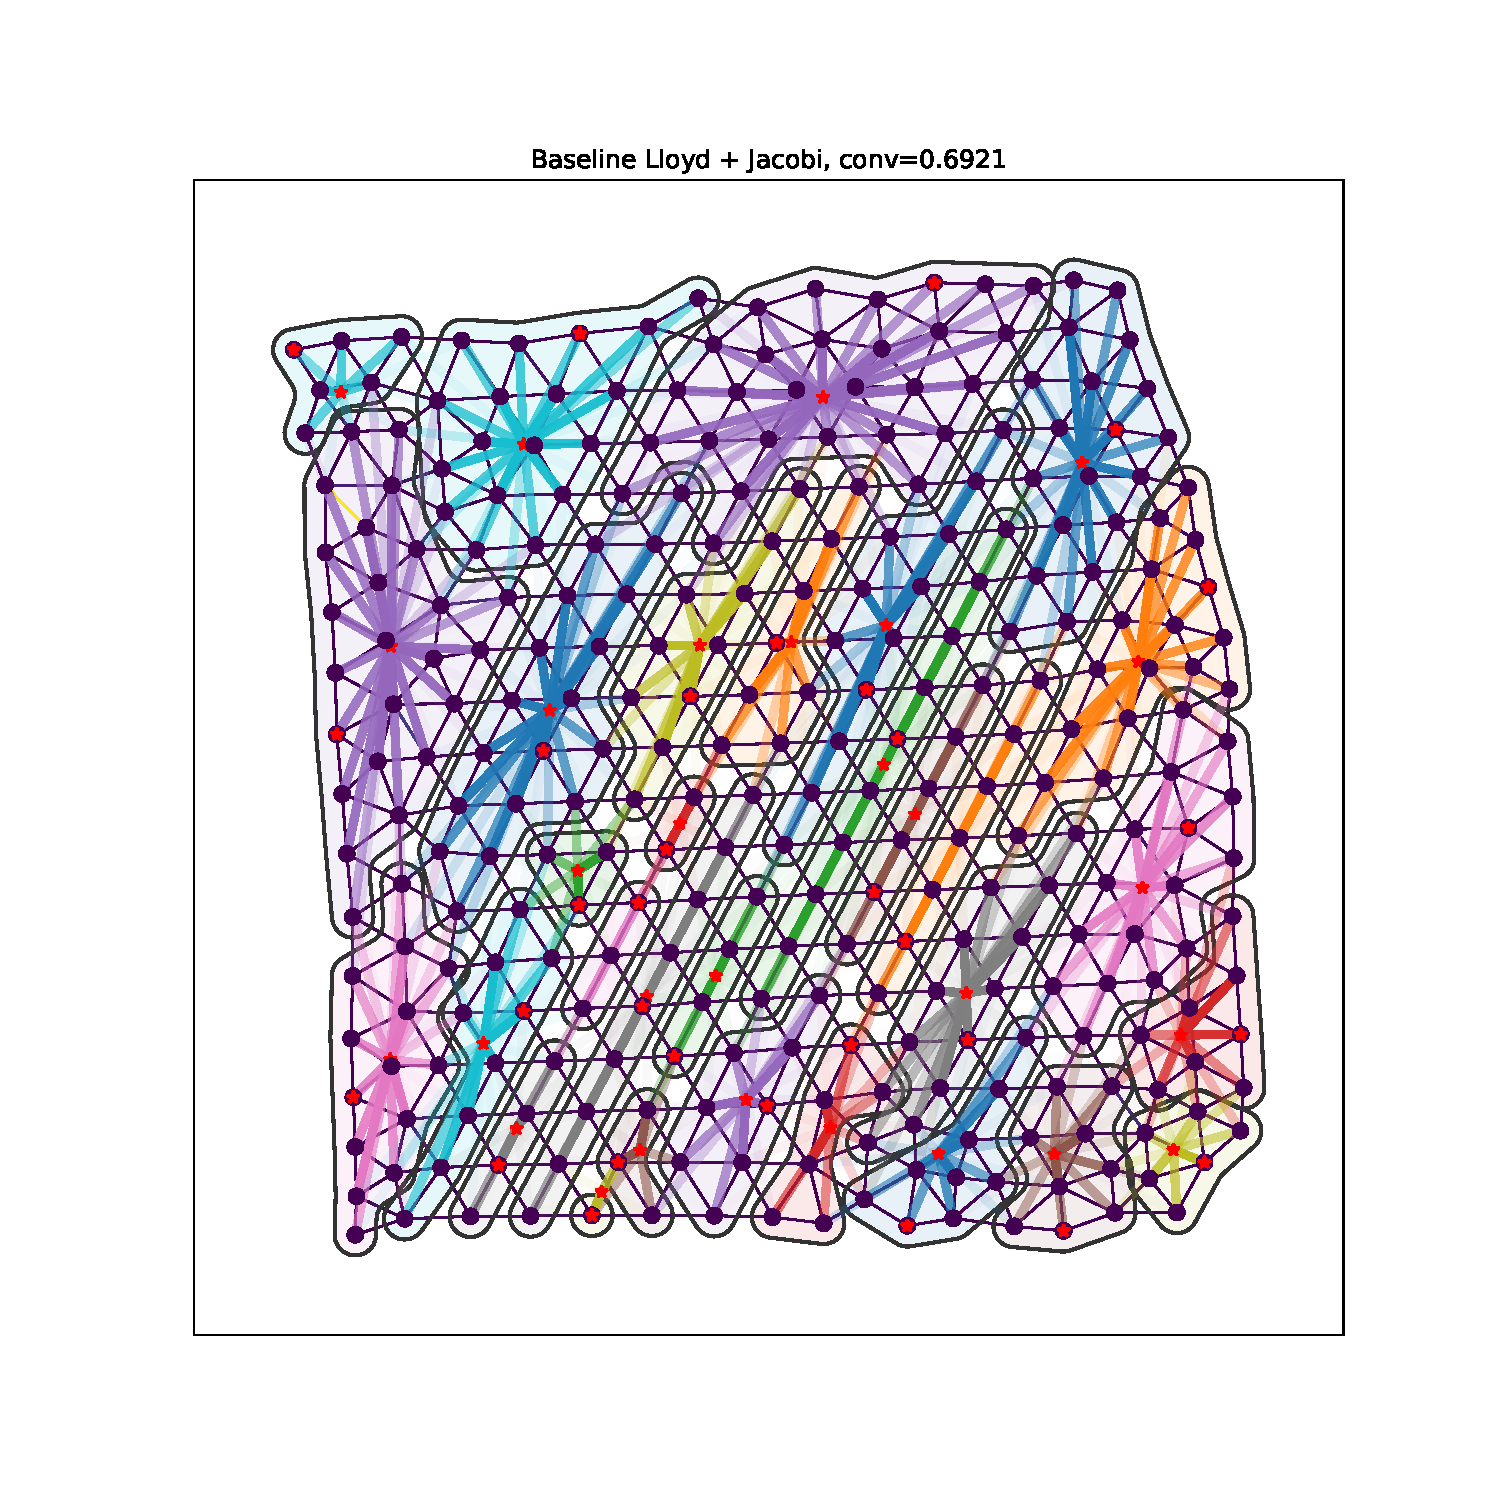
\includegraphics[width=\textwidth, trim=80 70 70 50, clip]{grid_anis_4_lloyd.pdf}
    \caption{Lloyd + Jacobi}
  \end{subfigure}
  \begin{subfigure}[t]{0.32\textwidth}
    \centering
    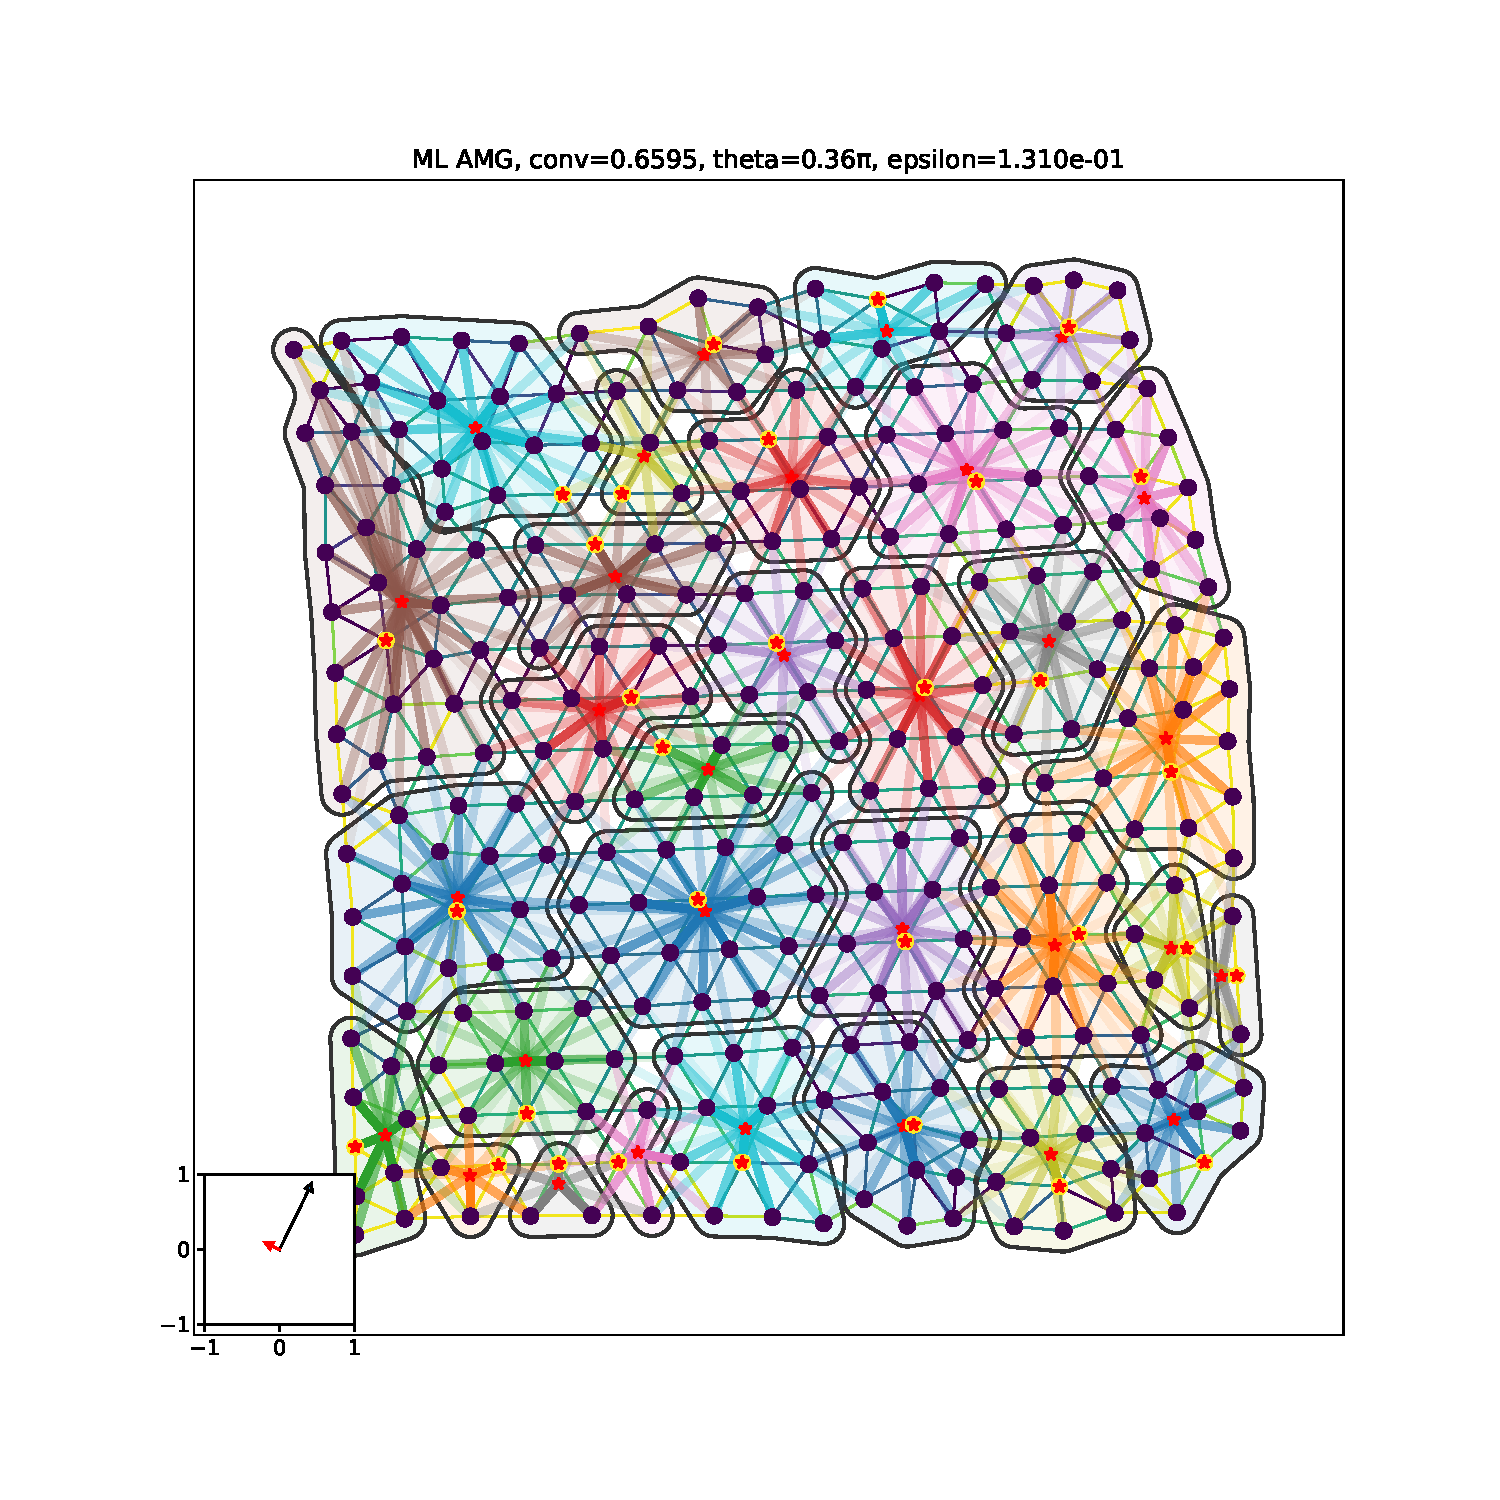
\includegraphics[width=\textwidth, trim=80 70 70 50, clip]{grid_anis_4_ml.pdf}
    \caption{ML}
  \end{subfigure}
  \caption{Aggregate and interpolation data for a random anisotropic mesh.  This is a different network from the isotropic case.}
  \label{fig:grid_anis_4}
\end{figure}

\begin{figure}[h]
  \centering
  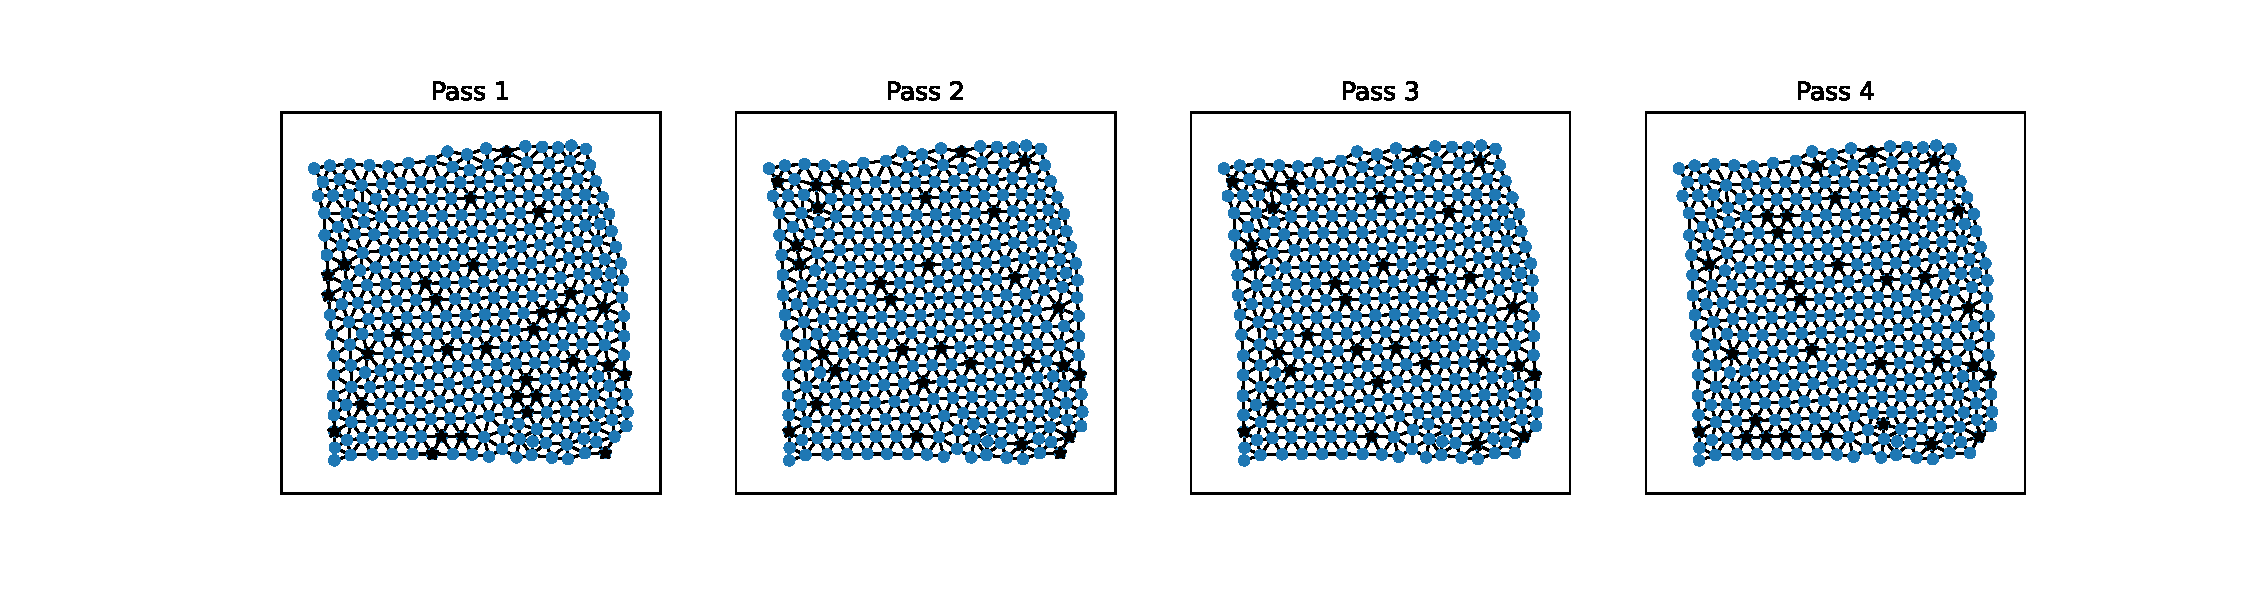
\includegraphics[width=\textwidth, trim=120 0 100 0, clip]{grid_anis_4_agg_pass.pdf}
  \caption{Tentative aggregate centers after each binarization ``pass''.  This is the same mesh as in figure \ref{fig:grid_anis_4}.}
\end{figure}

\begin{figure}[h]
  \centering
  \begin{subfigure}[t]{0.32\textwidth}
    \centering
    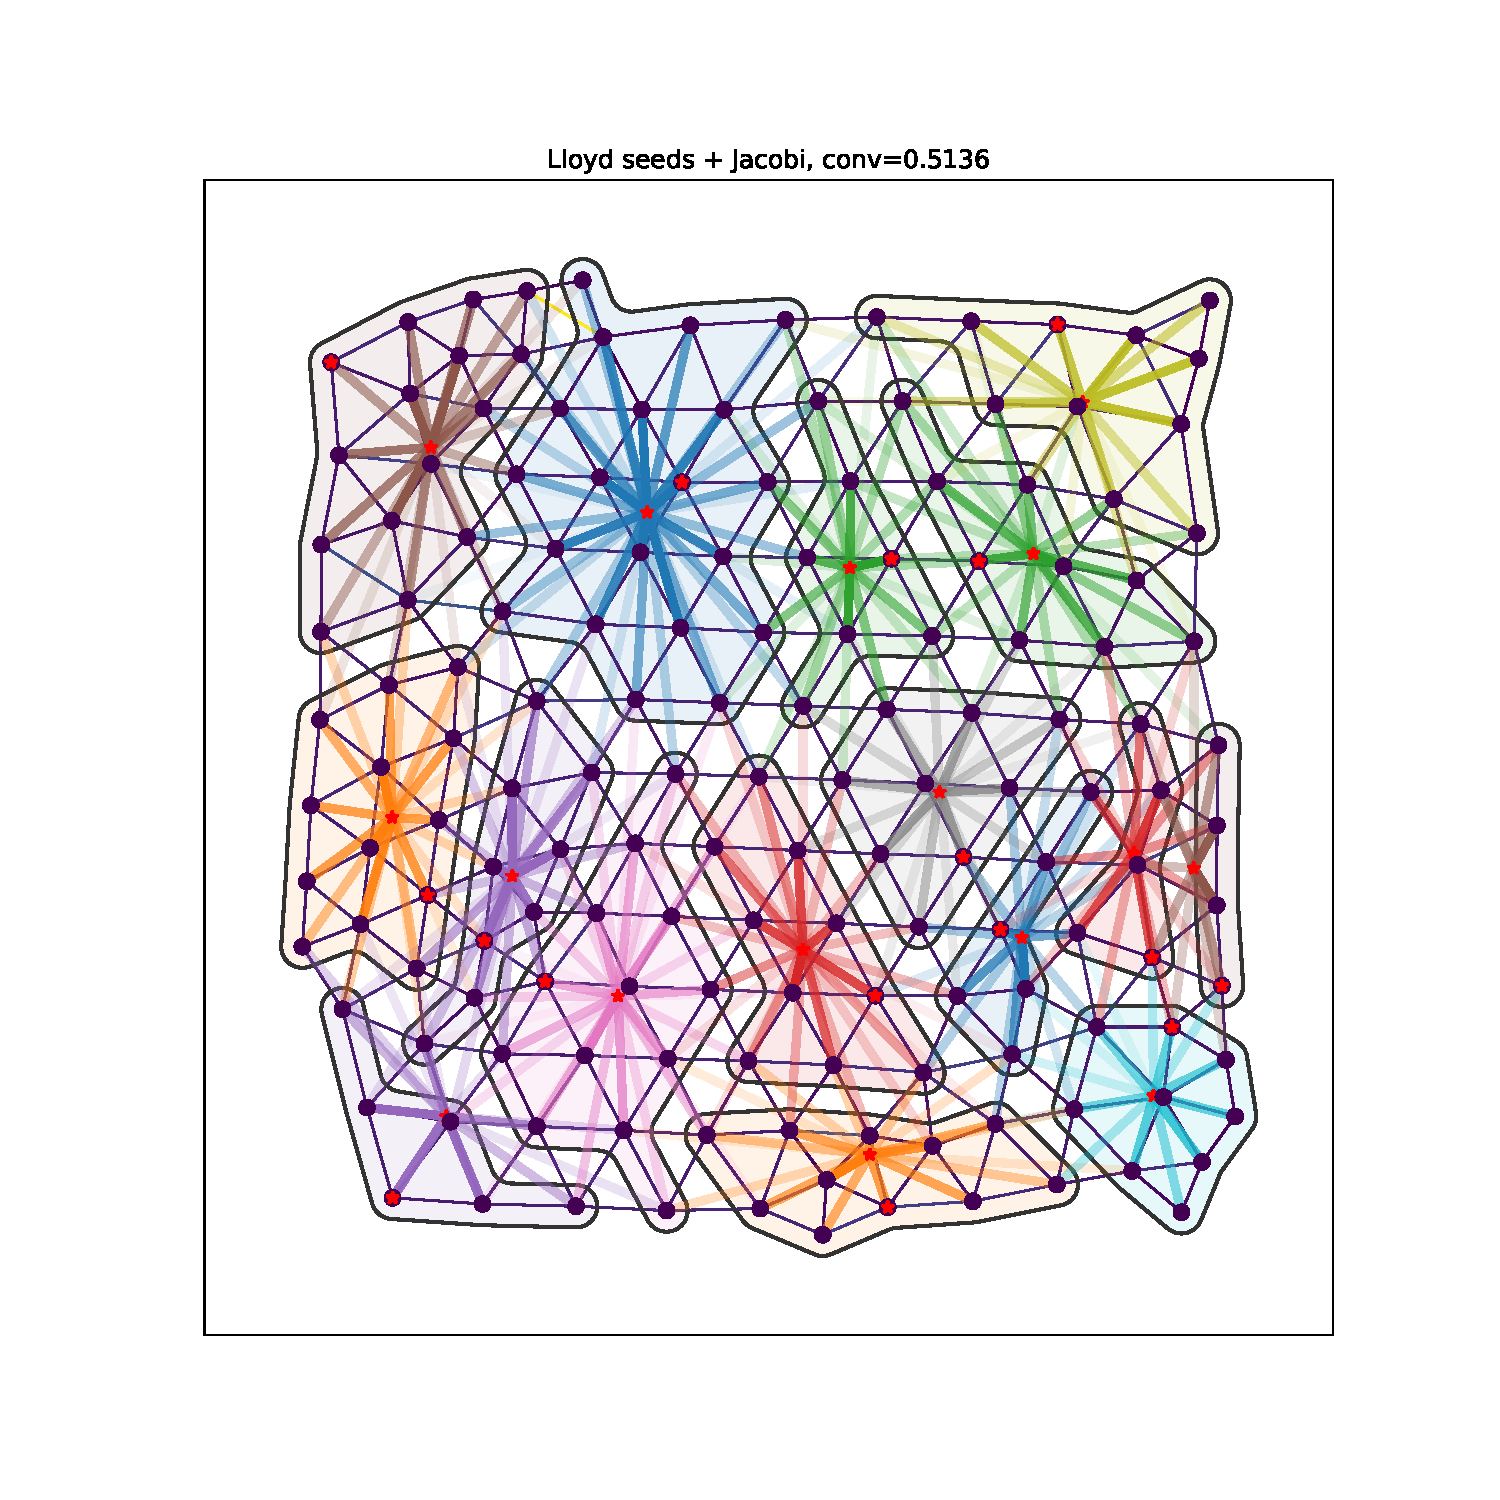
\includegraphics[width=\textwidth, trim=80 70 70 50, clip]{grid_anis_8_dumb.pdf}
    \caption{Initial Lloyd Configuration}
  \end{subfigure}
  \begin{subfigure}[t]{0.32\textwidth}
    \centering
    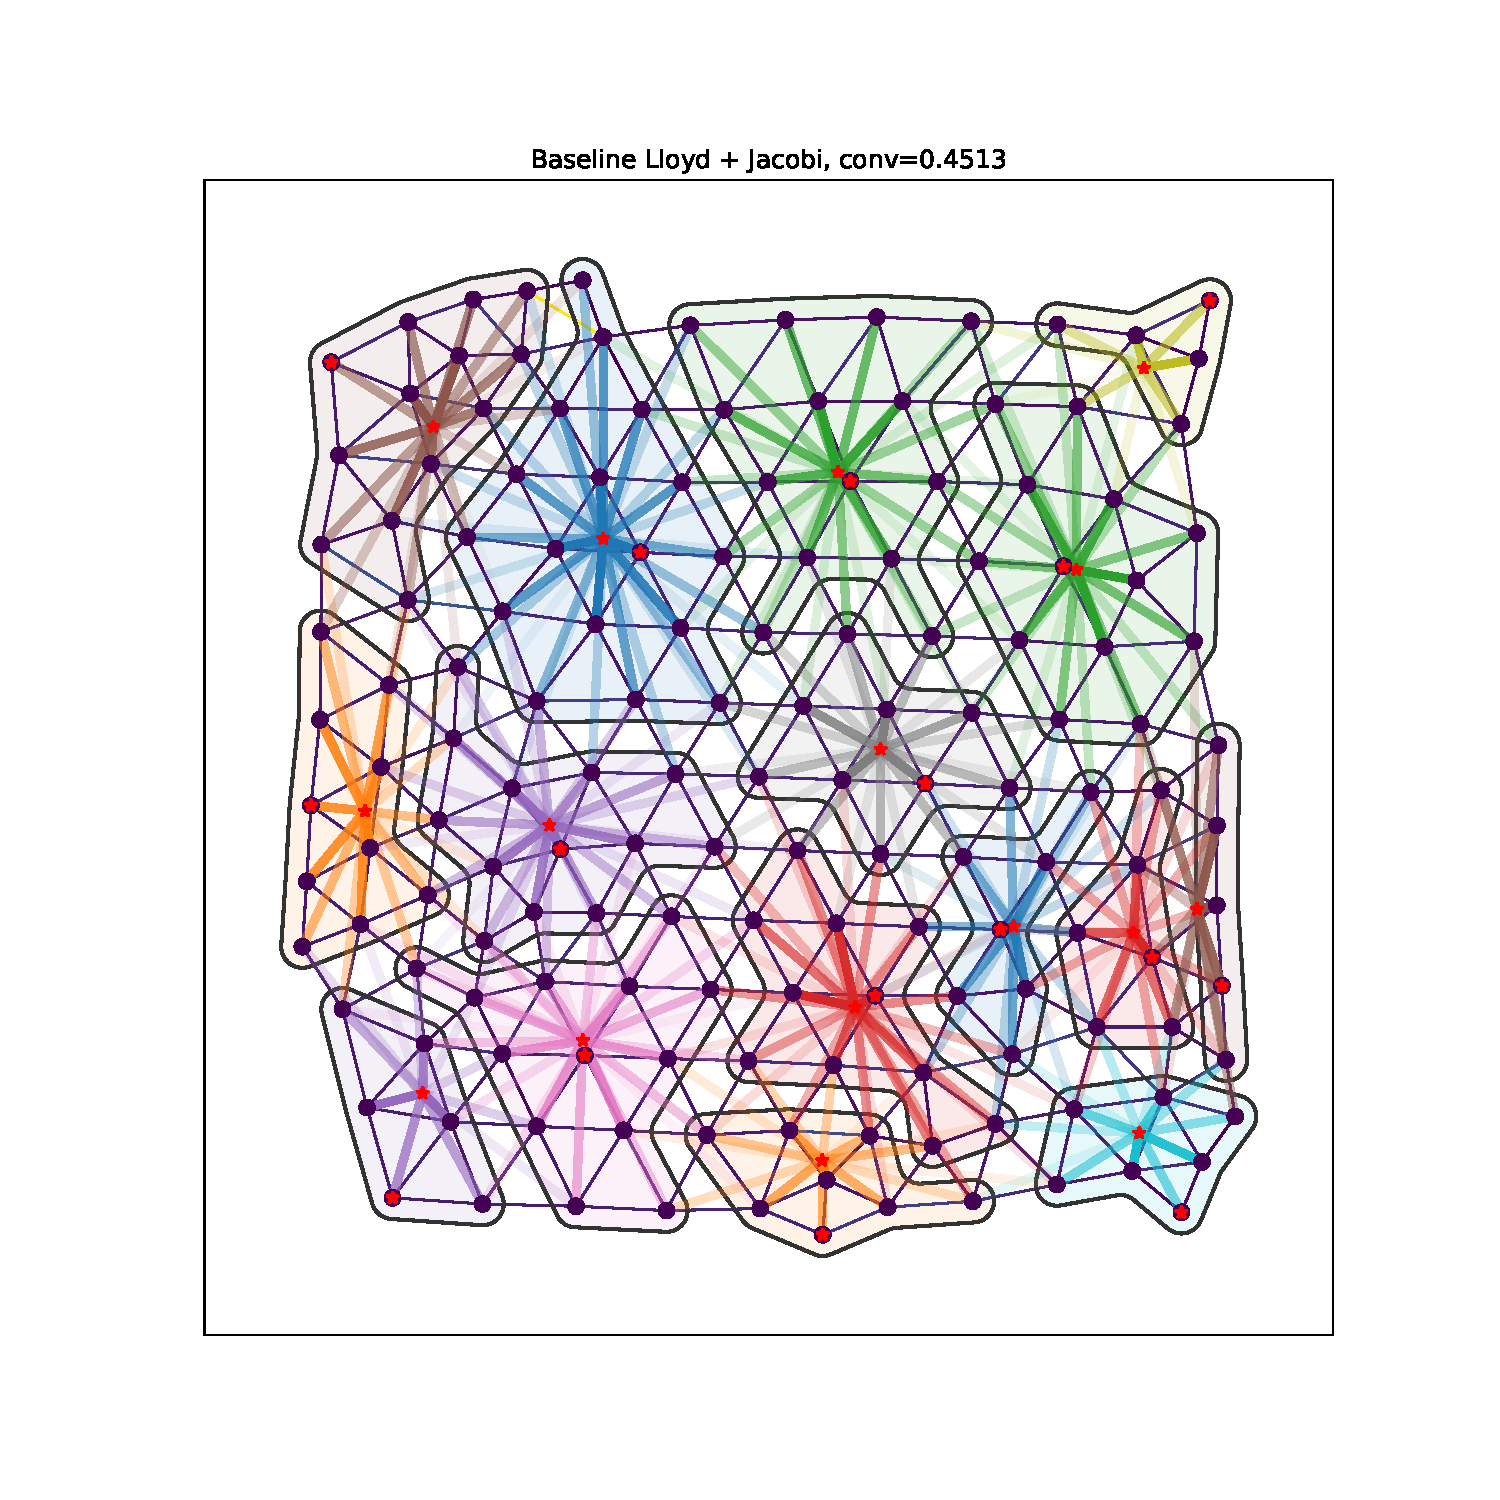
\includegraphics[width=\textwidth, trim=80 70 70 50, clip]{grid_anis_8_lloyd.pdf}
    \caption{Lloyd + Jacobi}
  \end{subfigure}
  \begin{subfigure}[t]{0.32\textwidth}
    \centering
    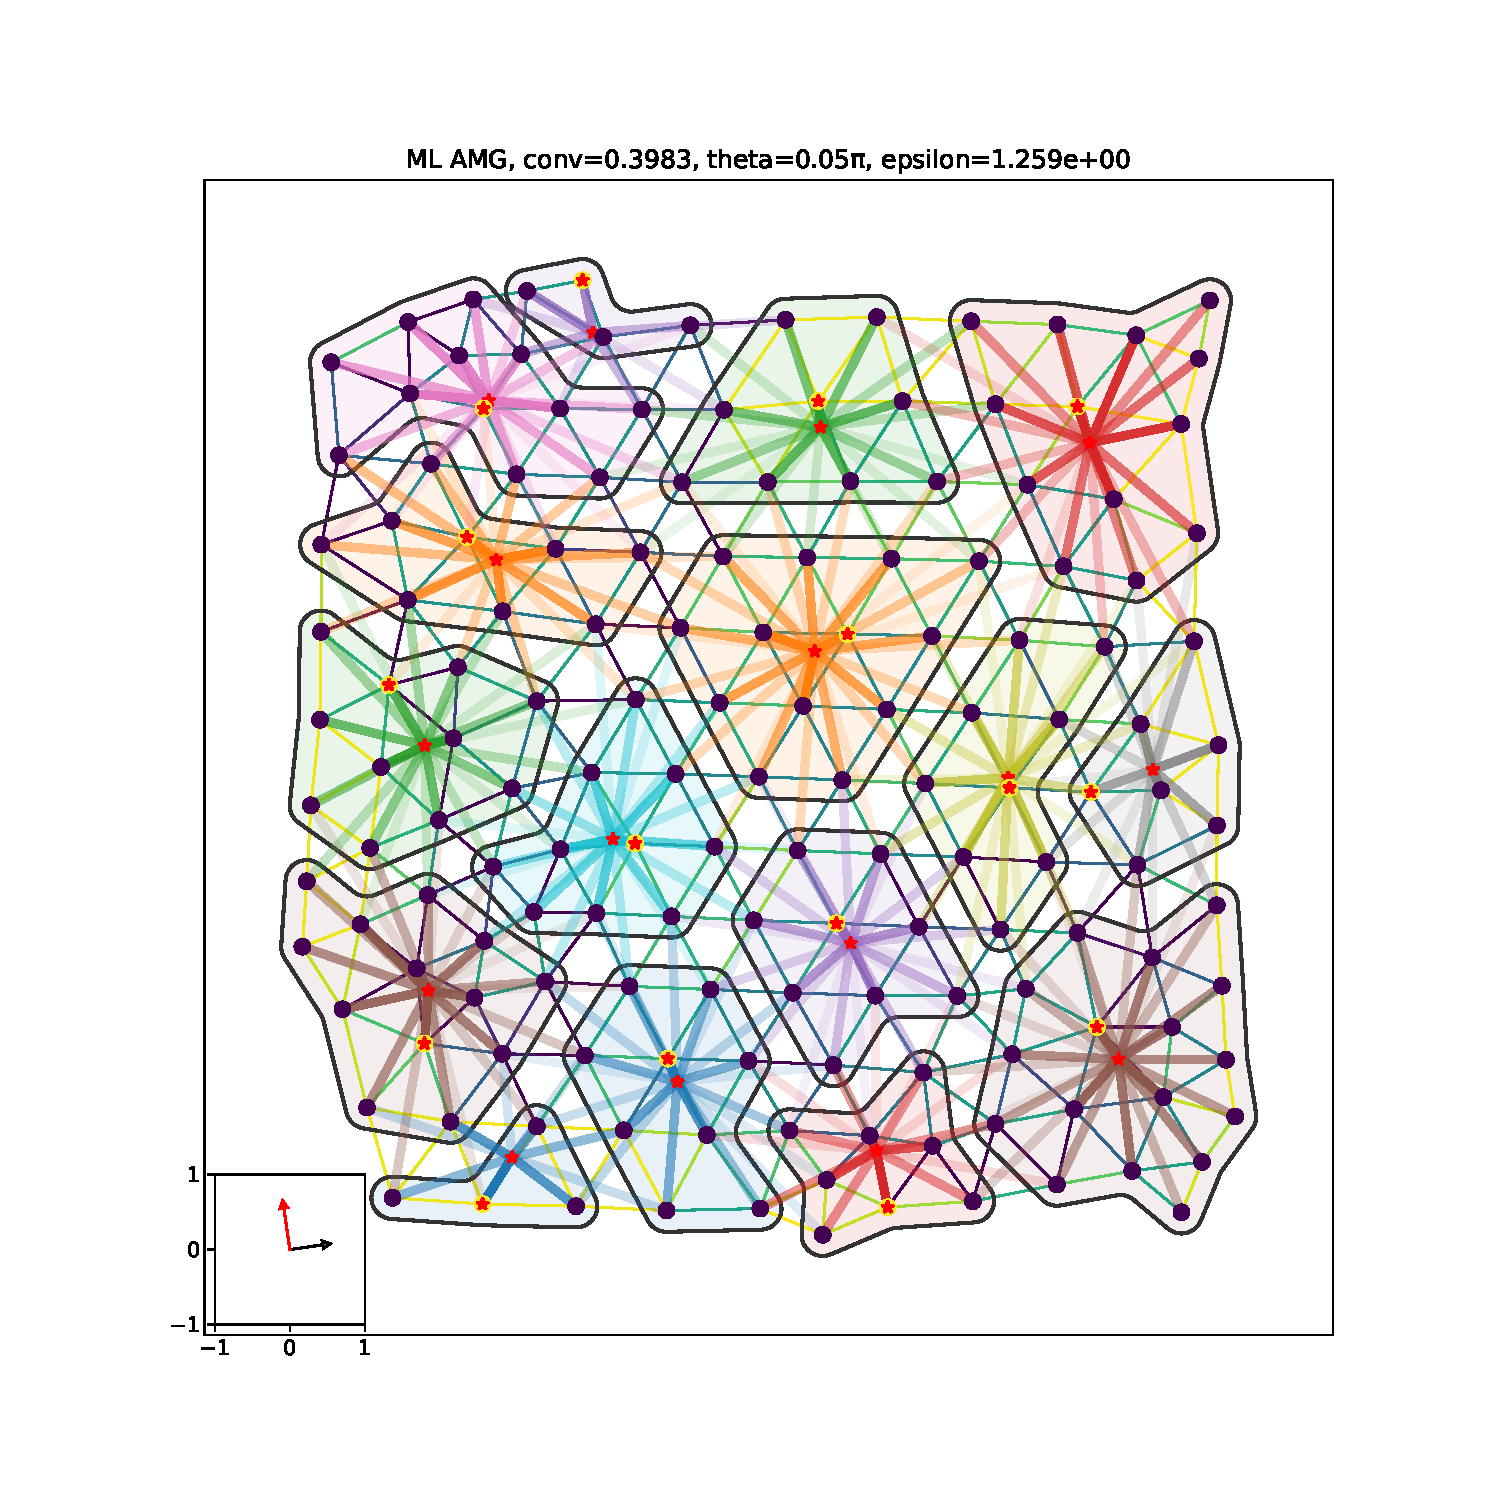
\includegraphics[width=\textwidth, trim=80 70 70 50, clip]{grid_anis_8_ml.pdf}
    \caption{ML}
  \end{subfigure}
  \caption{Aggregate and interpolation data for a random anisotropic mesh.  This is a different network from the isotropic case.}
  \label{fig:grid_anis_8}
\end{figure}

\begin{figure}[h]
  \centering
  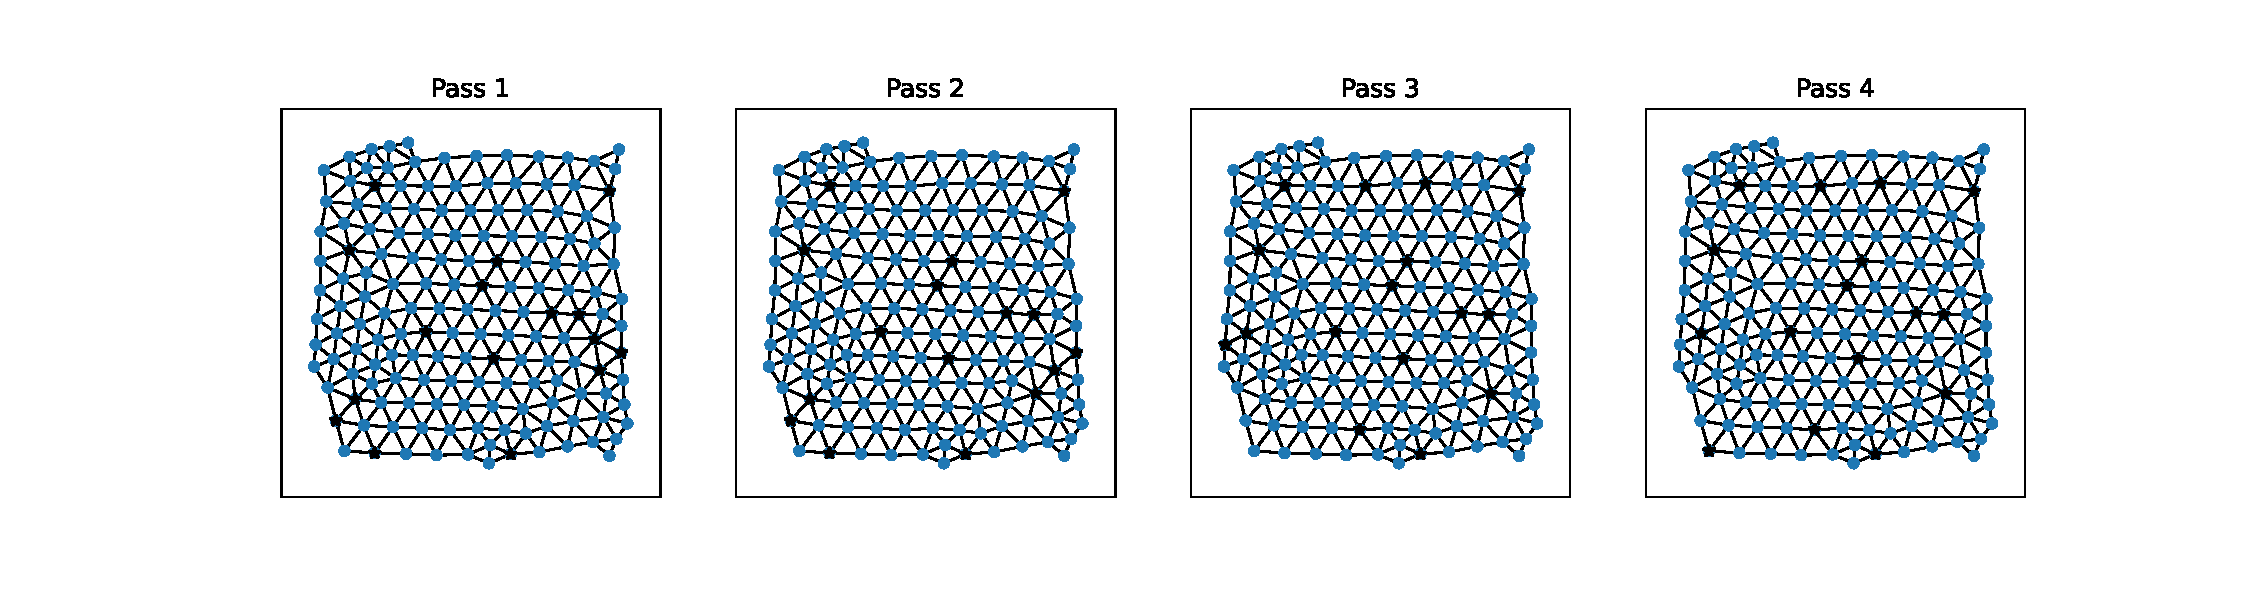
\includegraphics[width=\textwidth, trim=120 0 100 0, clip]{grid_anis_8_agg_pass.pdf}
  \caption{Tentative aggregate centers after each binarization ``pass''.  This is the same mesh as in figure \ref{fig:grid_anis_8}.}
\end{figure}

\bibliographystyle{siam}
\bibliography{navier}
\end{document}
